\documentclass[12pt, twoside=semi,openright,numbers=noenddot,titlepage=false]{scrbook}
\usepackage[spicy, fancy, book, solutions]{rishubh}

\title{Complex Analysis}

\begin{document}

\frontmatter
% \renewcommand{\thepage}{\arabic{page}}
\maketitle

\chapter*{Preface}
The following is a collection of notes I compiled while reading through Lars Ahlfors' classic text \textit{Complex Analysis} during the summer of 2025, in preparation of Stanford's MATH 116 course of the same name.

The quarter system at Stanford, in my opinion, is not optimal for a mathematics degree: a semester's worth of material is crammed into ten weeks of instruction, with a midterm and final exam. Because of this insanely fast pace, I have found that I learn mathematics best when I prepare independently of coursework, taking the time to absorb the concepts with no pressure of handing in assignments every week.

To that end, this forms part of a series of notes I intend to organize on an array of upper-level subjects, including algebraic topology, algebraic geometry, and differential topology.

\mainmatter

\tableofcontents

\part{Complex Numbers}
\chapter{The Algebra of Complex Numbers}
\label{chap:complex-algebra}

This chapter will mostly be review from high-school algebra, and also a way to flex calculation muscles and peel off the rust after not working with complex numbers in a while.

\section{Arithmetic Operations}
We define the \emph{imaginary unit $i$} as a quantity that obeys the property $i^2=-1$. By taking the linear span of the set $\{1,i\}$ over real coefficients, we produce a new mathematical object:

\begin{definition}
A \emph{complex number} is of the form $a+bi$, with $a,b \in \RR$, where $a$ and $b$ are the \emph{real} and \emph{imaginary} parts of the complex number, respectively.
\end{definition}

If we are well-acquainted with basic abstract algebra, then we note that the complex number system, denoted by $\CC=\{a+bi \colon a,b \in \RR\}$, can also be thought of as the quotient $\RR[t]/(t^2+1)$; that is, the ring of polynomials with real coefficients modulo the quadratic $t^2+1$. It should be clear, then, that the degree of $\CC$ over $\RR$, written $[\CC \colon \RR]$, is equal to $2$. In other words, the complex numbers form a quadratic field extension of the real numbers.

In fact, the field $\CC$ is \textit{algebraically closed}, meaning that every polynomial with real coefficients has a root in $\CC$. There are a number of proofs of this fact, called the Fundamental Theorem of Algebra, but my favorite is the one by Milnor via differential topology.

Back to arithmetic. If $a=0$, then we call $a+bi$ \emph{purely imaginary}, and if $b=0$, then -- of course -- $a+bi$ is \textit{real}.

Addition of two complex numbers is defined component-wise: $$(a+bi)+(c+di)=(a+c)+(b+d)i,$$ while multiplication is carried out distributively, keeping in mind the fundamental property that $i^2=-1$:
\begin{align*}
	(a+bi)(c+di) &=ac+adi+bci+bdi^2 \\
	&=ac+(ad+bc)i-bd \\
	&=(ac-bd)+(ad+bc)i.
\end{align*}

We remember from high school that two complex numbers may also be divided by mutiplying both the numerator and denominator by the conjugate of the denominator to realize the denominator:
\begin{align*}
	\dfrac{a+bi}{c+di} &=\dfrac{a+bi}{c+di} \cdot \dfrac{c-di}{c-di} \\
	&=\dfrac{(ac+bd)+(bc-ad)i}{c^2+d^2} \\
	&=\dfrac{ac+bd}{c^2+d^2}+\dfrac{bc-ad}{c^2+d^2}i.
\end{align*}

\begin{exercise}
	If $z=a+bi$, then find the real and imaginary parts of the complex number $\frac{z-1}{z+1}$.
	
	\begin{sol}
		Define the complex numbers $z'=z-1=(a-1)+bi$ and $z''=z+1=(a+1)+bi$, and set $w=\frac{z-1}{z+1}=\frac{z'}{z''}$. Then by the formula for division, we have
		\begin{align*}
			\Real w &=\dfrac{(a-1)(a+1)+b^2}{(a+1)^2+b^2} \\
			&=\boxed{\dfrac{a^2+b^2-1}{a^2+b^2+2a+1}},
		\end{align*}
		and
		\begin{align*}
			\Imag w &=\dfrac{b(a+1)-(a-1)b}{(a+1)^2+b^2} \\
			&=\boxed{\dfrac{2b}{a^2+b^2+2a+1}}.
		\end{align*}
	\end{sol}
\end{exercise}

\section{Square Roots}
Here, we give a procedure for finding the square root of a complex number. Let $z=a+bi$, and suppose $w \in \CC$ with $w^2=z$. Say that $w=x+yi$; then, write $$(x+yi)^2=a+bi \then (x^2-y^2)+2xyi=a+bi.$$ Equating real and imaginary parts yields the system of equations
\begin{align*}
	x^2-y^2 &=a, \\
	2xy &=b.
\end{align*}

Substituting $y=b/2x$ into the first equation gives
\begin{align*}
	x^2-\left(\dfrac{b}{2x}\right)^2 &=a \\
	\then x^2-\dfrac{b^2}{4x^2} &=a,\\
	\then 4x^4-4ax^2-b^2 &=0,
\end{align*}
so $$x^2=\dfrac{4a+4\sqrt{a^2+b^2}}{8}=\dfrac{a+\sqrt{a^2+b^2}}{2}.$$ We take the positive square root of the discriminant in the quadratic formula because $\sqrt{a^2+b^2} \ge a$, and we want $x$ to be real.

From this, we also get $$y^2=x^2-a=\dfrac{-a+\sqrt{a^2+b^2}}{2}.$$ Now, we can take either the positive or the negative square root to get two opposite values of $x$ and $y$, but we must be careful, as these values cannot be multiplied arbitrarily -- they must multiply to the sign of $b$. Hence, instead of $4$ square roots, we do get the anticipated $2$, namely, $$w=x+yi=\pm \left(\sqrt{\dfrac{a+\sqrt{a^2+b^2}}{2}}+\sign(b)\sqrt{\dfrac{-a+\sqrt{a^2+b^2}}{2}}i\right),$$ provided $b \neq 0$. If $b=0$, then simply $$w=\pm \sqrt{a}, \quad a \ge 0,$$ or $$w=\pm i\sqrt{-a}, \quad a<0.$$

\begin{exercise}
	Compute $\sqrt[4]{i}$.
	
	\begin{sol}
		We don't have access to the geometric interpretation of complex numbers yet, so we'll content ourselves to solve this problem algebraically.
		
		First, let us find $\sqrt{i}$: we have $\Real i=0$ and $\Imag i=1$, so
		\begin{align*}
			\sqrt{i} &=\pm\left(\sqrt{\dfrac{1}{2}}-\sqrt{\dfrac{1}{2}}i\right) \\
			&=\pm\left(\dfrac{1-i}{\sqrt{2}}\right).
		\end{align*}
		
		Now, we get two additional square roots each of $1-i$ and $-1+i$, which are
		\begin{align*}
			\sqrt{-1+i} &=\pm\left(\sqrt{\dfrac{1+\sqrt{2}}{2}}-\sqrt{\dfrac{-1+\sqrt{2}}{2}}i\right) \\
			&=\pm\left(\dfrac{\sqrt{1+\sqrt{2}}-i\sqrt{-1+\sqrt{2}}}{\sqrt{2}}\right),
		\end{align*}
		and
		\begin{align*}
			\sqrt{1-i} &=\pm\left(\sqrt{\dfrac{-1+\sqrt{2}}{2}}+\sqrt{\dfrac{1+\sqrt{2}}{2}}i\right) \\
			&=\pm\left(\dfrac{\sqrt{-1+\sqrt{2}}+i\sqrt{1+\sqrt{2}}}{\sqrt{2}}\right),
		\end{align*}.
		Therefore,
		\begin{align*}
			\sqrt[4]{i} &=\boxed{\left\{\pm\left(\dfrac{\sqrt{1+\sqrt{2}}-i\sqrt{-1+\sqrt{2}}}{\sqrt[4]{2}}\right), \pm\left(\dfrac{\sqrt{-1+\sqrt{2}}+i\sqrt{1+\sqrt{2}}}{\sqrt[4]{2}}\right)\right\}}.
		\end{align*}
	\end{sol}
\end{exercise}

\section{Conjugation and Absolute Value}
We mentioned the conjugate of a complex number in the first section. Here, we make the notion precise:

\begin{definition}
	The \textit{conjugate} of the complex number $z=a+bi$ is the complex number $\overline{z}=a-bi$. 
\end{definition}

\begin{definition}
	The \emph{absolute value}, or \emph{norm}, of the complex number $z=a+bi$ is the positive real-valued quantity $$\abs{z}=\sqrt{z\overline{z}}=\sqrt{(a+bi)(a-bi)}=\sqrt{a^2+b^2}.$$
\end{definition}

Note the following properties of conjugation and absolute value, for $z,w \in \CC$:
\begin{itemize}
	\item $\overline{z+w}=\overline{z}+\overline{w}$,
	\item $\overline{zw}=\overline{z} \cdot \overline{w}$,
	\item $\Real z=\dfrac{z+\overline{z}}{2}$,
	\item $\Imag z=\dfrac{z-\overline{z}}{2i}$, and
	\item $\abs{zw}=\abs{z} \cdot \abs{w}$.
\end{itemize}

It should be clear that the absolute value is multiplicative; that is, for any $z,w \in \CC$ ,we have $$\abs{zw}=\abs{z} \cdot \abs{w}.$$

\begin{exercise}
	Prove that $\left\abs{\dfrac{w-z}{1-\overline{w}z}\right}=1$ if either $\abs{w}=1$ or $\abs{z}=1$. What happens when $\abs{w}=\abs{z}=1$?
	
	\begin{sol}
		Suppose, without loss of generality, that $\abs{w}=1$ and $\abs{z} \neq 1$. Note that, in this case, $\overline{w}b \neq 1$, so we are not dividing by $0$. This is because if it was equal to $1$, then we would have $a\overline{z}=\overline{1}=1$, so that $\overline{w}zw\overline{z}=\overline{w}w\overline{z}z=\abs{w}\abs{z}=\abs{z}=1$, which is assumed not to be true.
		
		Next, observe that $\abs{wz}=\abs{z}$, so we have
		\begin{align*}
			\left\abs{\dfrac{w-z}{1-\overline{w}z}\right}^2 &=\dfrac{w-z}{1-\overline{w}z} \cdot \dfrac{\overline{w}-\overline{z}}{1-w\overline{z}} \\
			&=\dfrac{\abs{w}+\abs{z}-w\overline{z}-\overline{w}z}{1-w\overline{z}-\overline{w}z+\abs{wz}} \\
			&=\dfrac{1-w\overline{z}-\overline{w}w+\abs{z}}{1-w\overline{z}-\overline{w}z+\abs{z}} \\
			&=1.
		\end{align*}
		
		On the other hand, if $\abs{w}=\abs{z}=1$, then the identity also holds, provided that $\overline{w}z \neq 1$.
	\end{sol}
\end{exercise}

\section{Useful Inequalities}
There is no standard order imposed on the complex number system, but we can extract some valuable inequalities by comparing real and imaginary parts and by taking absolute values to transfer computations into the real number system.

We first note that, since $\abs{z}^2=(\Real z)^2+(\Imag z)^2$, we can immediately say that
\begin{align*}
	-\abs{z} &\le \Real z \le \abs{z}, \text{ and } \\
	-\abs{z} &\le \Imag z \le \abs{z}.
\end{align*}

Observe that
\begin{align*}
	\abs{w+z}^2 &=(w+z)(\overline{w}+\overline{z}) \\
	&=w\overline{w}+w\overline{z}+\overline{w}z+z\overline{z} \\
	&=\abs{w}+\abs{z}+w\overline{z}+\overline{w\overline{z}} \\
	&=\abs{w}+\abs{z}+2\Real(w\overline{z}) \\
	&\le \abs{w}+\abs{z}+2\abs{w\overline{z}} \\
	&=\abs{w}+\abs{z}+2\abs{wz} \\
	&=\left(\abs{w}+\abs{z}\right)^2,
\end{align*}
so taking square roots gives 
\begin{proposition}[Triangle Inequality]
	\label{prop:triangle-inequality}
	For any complex numbers $z,w$, we have $$\abs{w+z} \le \abs{w}+\abs{z}.$$
\end{proposition}

Note that, by the derivation, equality holds if and only if $\Real(w\overline{z})=\abs{wz}$, or that $w\overline{z}$ is real and positive. Writing $w=a+bi$ and $z=c+di$, we find that $$w\overline{z}=(ac+bd)+(-ad+bc)i$$ is real implies that $ad=bc$, or that $a/c=b/d$. In other words, $w$ and $z$ differ by a positive real number.

We can extend this reasoning by induction to show that for any finite set of complex numbers $\{z_1,z_2,\dots,z_n\}$, we have $$\abs{z_1+z_2+\cdots+z_n} \le \abs{z_1}+\abs{z_2}+\cdots+\abs{z_n},$$ with \textit{equality holding if and only if the ratio of any two nonzero terms is a positive real number.}

Notice that, expressed another way, the triangle inequality becomes $$\abs{w-z}+\abs{z} \le \abs{(w-z)+z}=\abs{w},$$ and rearranging gives $$\abs{w}-\abs{z} \ge \abs{w-z}.$$ Swapping the roles of $w$ and $z$ results in $$\abs{z}-\abs{w} \ge \abs{z-w}=\abs{w-z},$$ so we can combine these two inequalities to get $$\abs{w-z} \le \abs{\abs{w}-\abs{z}}.$$ Of course, the same estimate can easily be applied to $\abs{w+z}$.

We conclude this section with another famous and extremely useful inequality.

\begin{theorem}[Cauchy-Schwarz Inequality]
	\label{thm:cauchy-schwarz}
	Given $z_1,\dots,z_n$ and $w_1,\dots,w_n$, the following holds: $$\abs{w_1z_1+\cdots+w_nz_n}^2 \le \left(\abs{w_1}^2+\cdots+\abs{w_n}^2\right) \cdot \left(\abs{z_1}^2+\cdots+\abs{z_n}^2\right).$$
\end{theorem}

\begin{proof}
	We proceed by induction on $n$. For $n=1$, it is obvious that $$\abs{w_1z_1}^2=\abs{w_1}^2\abs{z_1}^2,$$ so assume the result to be true for some $n \ge 1$.
	
	Then, by the triangle inequality,
	\begin{align}
		\abs{w_1z_1+\cdots+w_nz_n+w_{n+1}z_{n+1}}^2 &\le \left(\abs{w_1z_1+\cdots+w_nz_n}+\abs{w_{n+1}z_{n+1}}\right)^2 \nonumber \\
		&=\abs{w_1z_1+\cdots+w_nz_n}^2 \nonumber \\&+2\abs{w_1z_1+\cdots+w_nz_n}\abs{w_{n+1}z_{n+1}}+\abs{w_{n+1}}^2\abs{z_{n+1}}^2 \nonumber \\
		&\le \left(\abs{w_1}^2+\cdots+\abs{w_n}^2\right) \cdot \left(\abs{z_1}^2+\cdots+\abs{z_n}^2\right) \nonumber \\&+2\abs{w_1z_1+\cdots+w_nz_n}\abs{w_{n+1}z_{n+1}}+\abs{w_{n+1}}^2\abs{z_{n+1}}^2 & \text{(Induction)}.
	\end{align}
	Now, observe that, for all $1 \le i \le n$, we have $$0 \le \left(\abs{w_{n+1}z_i}-\abs{w_iz_{n+1}}\right)=\abs{w_{n+1}}^2\abs{z_i}^2-2\abs{w_{n+1}z_{n+1}w_iz_i}+\abs{w_i}^2\abs{z_{n+1}^2},$$ so $$2\abs{w_{n+1}z_{n+1}w_iz_i} \le \abs{w_{n+1}}^2\abs{z_i}^2+\abs{w_i}^2\abs{z_{n+1}^2}.$$ Hence, by the Triangle Inequality again,
	\begin{align}
		2\left\abs{\sum_{i=1}^{n}w_iz_i\right} \cdot \abs{w_{n+1}z_{n+1}} &\le 2\sum_{i=1}^{n}\abs{w_{n+1}z_{n+1}w_iz_i} \nonumber \\ &\le \sum_{i=1}^{n}\abs{w_{n+1}}^2\abs{z_i}^2+\sum_{i=1}^{n}\abs{w_i}^2\abs{z_{n+1}^2} \nonumber \\
		&=\abs{w_{n+1}}^2\sum_{i=1}^{n}\abs{z_i}^2+\abs{z_{n+1}}^2\sum_{i=1}^{n}\abs{w_i}^2.
	\end{align}
	
	Plugging (1.2) into (1.1) yields
	\begin{align*}
		\abs{w_1z_1+\cdots+w_nz_n+w_{n+1}z_{n+1}}^2 &\le \left(\abs{w_1}^2+\cdots+\abs{w_n}^2\right) \cdot \left(\abs{z_1}^2+\cdots+\abs{z_n}^2\right) \\&+2\abs{w_1z_1+\cdots+w_nz_n}\abs{w_{n+1}z_{n+1}}+\abs{w_{n+1}}^2\abs{z_{n+1}}^2 \\
		&\le \left(\abs{w_1}^2+\cdots+\abs{w_n}^2\right) \cdot \left(\abs{z_1}^2+\cdots+\abs{z_n}^2\right)+ \\ &+\abs{w_{n+1}}^2\left(\abs{z_1}^2+\cdots+\abs{z_n}^2\right)+\abs{z_{n+1}}^2\left(\abs{w_1}^2+\cdots+\abs{w_n}^2\right) \\ &+\abs{w_{n+1}}^2\abs{z_{n+1}}^2 \\
		&=\left(\abs{w_1}^2+\cdots+\abs{w_{n+1}}^2\right) \cdot \left(\abs{z_1}^2+\cdots+\abs{z_{n+1}}^2\right),
	\end{align*}
	completing the induction and proving the inequality.
\end{proof}

The Cauchy-Schwarz inequality can be proven more generally for inner product spaces, of which the complex numbers are one canonical example, but we will not be needing that form here.

Analysis frequently comes down to bounding, and one may be a bit surprised to learn that just these simple tools -- the triangle inequality and Cauchy-Schwarz inequality -- can go a long way towards most of our estimates. The running joke is that analysts can do a lot with few tools.

\begin{exercise}
	Prove that $$\left\abs{\dfrac{w-z}{1-\overline{w}z}\right}<1$$ if $\abs{w}<1$ and $\abs{z}<1$.
	
	\begin{sol}
		Note that $$0<(\abs{w}-1)(\abs{z}-1),$$ so $$\abs{w}+\abs{z}<1+\abs{wz}.$$ Adding $-(w\overline{z}+\overline{w}z)$ to both sides gives 
		\begin{align*}
		\abs{w}+\abs{z}-w\overline{z}-\overline{w}z &<1+\abs{wz}-w\overline{z}-\overline{w}z \\
		\Rightarrow (w-z)(\overline{w}-\overline{z}) &<(1-\overline{w}z)(1-w\overline{z}) \\
		\Rightarrow \abs{w-z}^2 &<\abs{1-w\overline{z}}^2 \\
		\Rightarrow \left\abs{\dfrac{w-z}{1-w\overline{z}}\right}^2 &<1 \\
		\Rightarrow \left\abs{\dfrac{w-z}{1-w\overline{z}}\right} &<1,
		\end{align*}
		as desired.
	\end{sol}
\end{exercise}


\chapter{The Geometry of Complex Numbers}
\label{chap:complex-geometry}

With respect to a given rectangular coordinate system in the plane, like Cartesian coordinates, the complex number $a+bi$ can be represented as the point $(a,b)$. The first coordinate, which is the $x$-axis, is the \textit{real axis}, while the second coordinate -- the $y$-axis -- is the \textit{imaginary axis}.

Ahlfors prefers to derive all analytical arguments from the axioms of real numbers, rather than from geometry, but I believe that the geometric representation of complex numbers is an asset that should be exploited as much as possible. Indeed, a few examples in this chapter should convince the reader of the power of interpreting complex numbers as points in the plane. In many cases, geometry can reduce the work of solving a complex number problem by half or more.

\section{Geometric Addition and Multiplication}
\label{sec:geometric-addition-and-multiplication}

By appreciating the structure of $\CC$ as a vector space over $\RR$, we can consider a complex point a vector extending from the origin $(0,0)$. Then addition and subtraction of two complex numbers is easily represented by addition and subtraction of vectors in the plane, as shown below (recall that vectors added head-to-tail):

\begin{figure}[h]
	\caption{Complex vector addtion and subtraction}
	\centering
	\begin{asy}
	    settings.outformat="pdf";
	    unitsize(2cm);
	    Label La = Label("$w$", position=MidPoint);
	    Label Lb = Label("$z$", position=MidPoint);
	    Label Laminusb = Label("$w-z$", position=Relative(0.25), filltype=Fill(white));
	    Label Laplusb = Label("$w+z$", position=Relative(0.75));
	    draw((0,0)--(2,1), arrow=Arrow(), L=La);
	    draw((0,0) -- (3,0), arrow=Arrow(), L=Laminusb);
	    draw((3,0) -- (2,1), arrow=Arrow(), L=Lb);
	    draw((1,-1) -- (0,0), arrow=Arrow(), L=Lb);
	    draw((1,-1) -- (3,0), arrow=Arrow(), L=La);
	    draw((1,-1) -- (2,1), arrow=Arrow, L=Laplusb);
	\end{asy}
\end{figure}

An additional benefit of the vector representation is that the length of the vector represented by $z$ is simply $\abs{z}$; hence, the distance between $w$ and $z$ is $\abs{w-z}$. With this, the triangle inequality's name is justified: $\abs{w+z} \le \abs{w}+\abs{z}$ is the geometric fact we know and love. Similarly, we can establish the \textit{parallelogram law} $\abs{w+z}^2+\abs{w-z}^2=2(\abs{w}^2+\abs{z}^2)$ (the sum of the squares of the diagonal lengths of a parallelogram is equal to the sum of hte squares of the side lengths).

In order to derive a geometric interpretation of the product of two complex numbers, we introduce polar coordinates, writing $$a+bi=r(\cos \theta+i \sin \theta),$$ where $r$ is the radial distance from the origin and $\theta$ is the angle that the vector representing $a+bi$ makes with the positive $x$-axis; it is frequently called the \emph{argument} of the complex number $z=a+bi$ and is denoted by $\arg z$ and is restricted to the range $[0,2\pi)$.

Given two complex numbers $w=r(\cos \alpha+i\sin \alpha)$ and $z=s(\cos \beta+i\sin \beta)$, their algebraic product is
\begin{align*}
	wz &=rs\left[\cos \alpha \cos\beta-\sin \alpha\sin\beta+(\sin \alpha\cos \beta+\sin \beta\cos \alpha)i\right] \\
	&=rs\left(\cos(\alpha+\beta)+\sin(\alpha+\beta)i\right),
\end{align*}
where we have used the well-known trigonometric sum identities. By the way, this establishes the following result:
\begin{proposition}
	\label{prop:argument-addition}
	Given two complex numbers $w$ and $z$, we have that $$\arg(wz)=\arg w+\arg z.$$
\end{proposition}

With this geometric result, drawing the product of two complex numbers in the plane is easy: in fact, we see -- as expected -- that the triangle formed by the vertices $0$, $1$, and $w$ is similar to the triangle formed by the vertices $0$, $z$, $wz$.

Division of complex numbers amounts to nearly the same thing: we have $$\arg\left(\dfrac{z}{w}\right)=\arg z-\arg w,$$ and the similar triangles are now $\{0,1,w\}$ and $\{0,z/w,z\}$.

\begin{figure}[h]
	\caption{Complex vector multiplication}
	\centering
	\begin{asy}
		settings.outformat="pdf";
		unitsize(3cm);
		
		Label Lw = Label("$w$", position=EndPoint);
		Label Lz = Label("$z$", position=EndPoint);
		Label Lwz = Label("$wz$", position=EndPoint);
		
		draw((0,0) -- (1,0), L=Label("$1$", position=EndPoint));
		draw((0,0) -- (sqrt(3)/2, 1/2), p=blue, L=Lw);
		draw((0,0) -- (1, sqrt(3)),p=blue, L=Lz);
		draw((0,0) -- (0,2),p=red, L=Lwz);
	\end{asy}
\end{figure}

\begin{exercise}
	Prove that the points $z_1,z_2,z_3$ are the vertices of an equilateral triangle if and only if $z_1^2+z_2^2+z_3^2=z_1z_2+z_2z_3+z_1z_3$.
	
	\begin{sol}
		If the points do form an equilateral triangle, then it is true that $z_3$ is the image of $z_1$ under a rotation of $\pi/3$ radians about $z_2$. So set $$w=\cos(\pi/3)+i\sin(\pi/3)=\dfrac{1}{2}+\dfrac{\sqrt{3}}{2}i,$$ and we have $$\dfrac{z_3-z_2}{z_1-z_2}=w.$$ Note that $\arg(w^6)=6\arg(w)=2\pi$, so $w^6=1$. Since this is the smallest power of $w$ that equals $1$, $w$ is a primitive sixth root of unity and satisfies $w^2-w+1=0$ (we could have arrived at this conclusion simply by applying Euler's formula $w=e^{\pi i/3}$, though that will be formally proved in the next few sections).
		
		Therefore,
		\begin{align*}
			\left(\dfrac{z_3-z_2}{z_1-z_2}\right)^2-\dfrac{z_3-z_2}{z_1-z_2}+1 &=0 \\
			\then (z_3-z_2)^2-(z_3-z_2)(z_1-z_2)+(z_1-z_2)^2 &=0 \\
			\then z_3^2-2z_2z_3+z_2^2-z_1z_3+z_2z_3+z_1z_2-z_2^2+z_1^2-2z_1z_2+z_2^2 &=0 \\
			\then z_1^2+z_2^2+z_3^2-z_1z_2-z_2z_3-z_1z_3 &=0 \\
			\then z_1^2+z_2^2+z_3^2 &=z_1z_2+z_2z_3+z_1z_3.
		\end{align*}
		
		The other direction is handled in the same way, as we can rearrange the relation $z_1^2+z_2^2+z_3^2=z_1z_2+z_2z_3+z_1z_3$ into the form above. First of all, either $z_1=z_2=z_3$ or no two of them are the same point, because if -- for example -- $z_1=z_3$, then plugging this in would transform the relation into $$z_1^2+z_3^2=2z_1z_3 \Rightarrow (z_1-z_3)^2=0,$$ so we would, in fact, have $z_1=z_2=z_3$.
		
		Thus, we can safely divide by $z_1-z_2$ and get that $(z_3-z_2)/(z_1-z_2)$ is a primitive sixth root of unity, meaning that it is simply the complex number corresponding to rotation by $\pi/3$ radians. \qedsymbol
	\end{sol}
\end{exercise}

\section{De Moivre's Formula and Roots of Unity}
\label{sec:de-moivre}
If the reader completed the previous exercise, then he or she would have already deduced the results we are about to state formally here. If $z=r(\cos \theta+i\sin \theta)$, then our work in the previous section immediately yields that $$z^n=r^n(\cos n\theta+i\sin n\theta)$$ for \textit{any} $n \in \ZZ$, as the case where $n$ is negative is easily verified by complex division.

For $r=1$, we obtain the special case
\begin{proposition}[De Moivre's Formula]
	\label{prop:de-moivre}
	Let $\theta \in [0,2\pi)$. Then $$(\cos \theta+i \sin \theta)^n=\cos n\theta+i \sin n \theta.$$
\end{proposition}

This identity allows us to find $n$th roots of complex numbers, for if $a=r(\cos \theta+i \sin \theta)$ and $z \in \CC$ with $z^n=a$, one easy candidate for $z$ is the number $$z=r^{1/n}\left(\cos\left(\theta/n\right)+i\sin(\theta/n)\right).$$ But shifting the argument by any multiple of $2\pi$ does not change the complex number, so we find that each of the numbers $$r^{1/n}\left(\cos\left(\dfrac{\theta+2\pi k}{n}\right)+i\sin\left(\dfrac{\theta+2\pi k}{n}\right)\right), \quad k=0,1,\dots,n-1$$ are also $n$th roots of $a$. Since $\CC$ is algebraically closed, the Fundamental Theorem of Algebra gives that the equation $z^n-a$ must have exactly $n$ complex roots, the ones enumerated above.

The equation $z^n=1$ is particularly important, and results in the $n$ \textit{$n$th roots of unity}. It is easy to check that they form a cyclic multiplicative group generated by the \textit{primitive} $n$th root of unity $$\zeta_n=\cos\left(\dfrac{2\pi}{n}\right)+i\sin\left(\dfrac{2\pi}{n}\right).$$ It is also quite clear that the solutions to the equation $z^n=a$ for any $a \in \CC$ are then $$\{\zeta_n^k\sqrt[n]{a} \colon k=0,1,\dots,n-1\},$$ where $\sqrt[n]{a}$ is any $n$th root of $a$.

Geometrically speaking, the $n$th roots of unity are the vertices of a regular $n$-gon centered at the origin.

\begin{exercise}
	Let $\omega$ be a primitive $n$th root of unity, and let $h$ be an integer such that $n$ does not divide $h$. What are the values of $$1+\omega^h+\omega^{2h}+\cdots+\omega^{(n-1)h}$$ and $$1-\omega^h+\omega^{2h}-\cdots+(-1)^{n-1}\omega^{(n-1)h}?$$
	
	\begin{sol}
		For the first expression, multiply both sides by $\omega^h-1$ to get
		\begin{align*}
			(1-\omega^h)(1+\omega^h+\omega^{2h}+\cdots+\omega^{(n-1)h}) &=1-\omega^{nh} \\
			&=1-(\omega^n)^h \\
			&=1-1 \\
			&=0.
		\end{align*}
		Since $\omega^h \neq 1$ (as $n \nmid h$), we must have $$1+\omega^h+\omega^{2h}+\cdots+\omega^{(n-1)h}=\boxed{0}.$$
		
		On the other hand, multiplying the second expression by $1+\omega^h$ gives
		\begin{align*}
			(1+\omega^h)(1-\omega^h+\omega^{2h}-\cdots+(-1)^{n-1}\omega^{(n-1)h}) &=1+(-1)^{n-1}\omega^{nh} \\
			&=1+(-1)^{n-1},
		\end{align*}
		so $$1-\omega^h+\omega^{2h}-\cdots+(-1)^{n-1}\omega^{(n-1)h} =\begin{cases}
			\dfrac{2}{1+\omega^h}, & n \text{ is odd}, \\
			0, & n \text{ is even}.
		\end{cases}.$$
	\end{sol}
\end{exercise}

\section{Analytic Geometry}
\label{sec:analytic-geometry}
In classical analytic geometry, the geometry of a locus is expressed as a relation between $x$ and $y$. In many geometry problems, such as those involving rectangles, squares, circles, angless that are multiples of $30^\circ$, the work is greatly simplified by translating to Cartesian coordinates. Complex coordinates can offer an even faster solution, since the equations are reduced to one variable and written in terms of $z$ and $\overline{z}$.

For instance, the equation of a circle of radius $r$ centered about the complex point $a$ is $\abs{z-a}=r$. This can be expanded as
\begin{align*}
	(z-a)(\overline{z}-\overline{a}) &=r^2 \\
	\then z\overline{z}-a\overline{z}-\overline{a}z+a\overline{a} &=r^2.
\end{align*}

A straight line in the complex plane can be given by the parametric form $$z=a+bt,$$ where $a,b \in \CC$, $b \neq 0$, and $t$ is the parameter running through all values in $\RR$. Two equations $z=a+bt$ and $z=a'+b't$ represent the same line if and only if $a'-a$ and $b'$ are real multiples of $b$. The lines are parallel whenever $b'$ is a real multiple of $b$, and they are equally directed if $b'$ is a positive multiple of $b$. The direction of a directed line can be identified with $\arg b$. The angle between $z=a+bt$ and $z=a'+b't$ is $\arg b'/b$, and in that sense, it is a directed angle. Hence, the lines are orthogonal (perpendicular) to each other if $b'/b$ is purely imaginary.

Note that, since $t$ is real, we can also write $\overline{z}=\overline{a}+\overline{b}t$, so that $$\overline{b}z-b\overline{z}-a\overline{b}+b\overline{a}=0.$$ This is the standard form of the equation of a line.

Problems of finding intersections between lines and circles, parallel or perpendicular lines, tangents, etc. usually become exceedingly simple when expressed in complex form. Mathematical competitions tend to feature such problems as brainteasers in ingenuity.

An inequality $\abs{z-a}<r$ describes the inside of a circle. Similarly, a directed line $z=a+bt$ determines a right half plane consisting of all points $z$ with $\Imag(z-a)/b<0$ and a left half plane with $\Imag(z-a)/b>0$.

\begin{exercise}
	Prove analytically that the midpoints of parallel chords to a circle lie on a diameter perpendicular to the chords.
	
	\begin{sol}
		Without loss of generality, let the circle have unit radius, and thus parametrize it by $\abs{z}=1$ in the complex plane. Let $a$ and $b$ be points on this circle; the chord between them is in the direction of $b-a$. Let $c$ be another point on the circle; we wish to find a point $d$ on the circle such that the chord between $c$ and $d$ is parallel to the chord between $a$ and $b$. Such a chord is represented by the parametric equation $c+t(b-a)$, so we want to solve for $d$ such that $d=c+t(b-a)$ for some real $t$, and $\abs{d}=1$. We then have
		\begin{align*}
			\left(c+t(b-a)\right) \cdot \left(\overline{c}+t(\overline{b}-\overline{a})\right) &=1.
		\end{align*}
		Making use of the fact that $\overline{z}=1/z$ for any point $z$ on the unit circle, we get
		\begin{align*}
			\left(c+t(b-a)\right)\cdot \left(\dfrac{1}{c}+t\left(\dfrac{1}{b}-\dfrac{1}{a}\right)\right) &=1 \\
			\then 1+ct\left(\dfrac{a-b}{ab}\right)+\dfrac{t}{c}\left(b-a\right)-t^2\left(\dfrac{(b-a)^2}{ab}\right) &=1 \\
			\then t(b-a)\left(-\dfrac{c}{ab}+\dfrac{1}{c}\right)-t^2\left(\dfrac{(b-a)^2}{ab}\right) &=0 \\
			\then t(b-a)\left[\left(\dfrac{ab-c^2}{abc}\right)-t\left(\dfrac{b-a}{ab}\right)\right] &=0 \\
			\then t &=\dfrac{ab-c^2}{abc} \cdot \dfrac{ab}{b-a} \\
			&=\dfrac{ab-c^2}{c(b-a)}.
		\end{align*}
		
		As a sanity check, we confirm that $t$ is real by taking its conjugate:
		\begin{align*}
			\overline{t} &=\dfrac{\overline{ab}-\overline{c}^2}{\overline{c}(\overline{b}-\overline{a})} \\
			&=\dfrac{\frac{1}{ab}-\frac{1}{c^2}}{\frac{1}{c}\left(\frac{1}{b}-\frac{1}{a}\right)} \\
			&=\dfrac{c^2-ab}{abc^2} \cdot \dfrac{a-b}{abc} \\
			&=\dfrac{c^2-ab}{c(a-b)} \\
			&=\dfrac{ab-c^2}{c(b-a)} \\
			&=t.
		\end{align*}
		Since $\overline{t}=t$, $t$ is real.
		
		Now,
		\begin{align*}
			d &=c+t(b-a) \\
			&=c+\dfrac{ab-c^2}{c(b-a)} \cdot (b-a) \\
			&=c+\dfrac{ab-c^2}{c} \\
			&=c+\dfrac{ab}{c}-c \\
			&=\dfrac{ab}{c}.
		\end{align*}
		We are in a position to determine the direction of the line formed by joining the midpoints of the two chords $ab$ and $cd$: it is
		\begin{align*}
			\dfrac{\frac{ab}{c}+c}{2}-\dfrac{a+b}{2} &=\dfrac{ab+c^2-ac-bc}{2c}.
		\end{align*}
		Since the direction of the chord formed by $a$ and $b$ is simply $b-a$, as mentioned above, it suffices to show by the discussion in the text that the quotient $$\dfrac{ab+c^2-ac-bc}{2c(b-a)}$$ is purely imaginary. Denote it by $w$ and take its conjugate:
		\begin{align*}
			\overline{w} &=\dfrac{\overline{ab}+\overline{c}^2-\overline{ac}-\overline{bc}}{2\overline{c}\left(\overline{b}-\overline{a}\right)} \\
			&=\dfrac{\frac{1}{ab}+\frac{1}{c^2}-\frac{1}{ac}-\frac{1}{bc}}{\frac{2}{c}\left(\frac{1}{b}-\frac{1}{a}\right)} \\
			&=\dfrac{c^2+ab-bc-ac}{abc^2} \cdot \dfrac{c}{2} \cdot \dfrac{ab}{a-b} \\
			&=\dfrac{ab+c^2-ac-bc}{2c(a-b)} \\
			&=-w.
		\end{align*}
		Hence, $w+\overline{w}=0$, so $\Real w=0$, and $w$ is purely imaginary.
		
		This is also true of the angle between the chord $cd$ and the line segment joining the midpoints of $ab$ and $cd$, since $cd \parallel ab$. We conclude that these two lines are perpendicular.
		
		To show that the center of the circle lies on the line joining the midpoints of $ab$ and $cd$ without resorting to the geometric fact that a radius perpendicular to the chord bisects that chord, we simply find the explicit parametrization of the line. Its direction is, of course, $\frac{ab+c^2-ac-bc}{2c}$, and since $\frac{a+b}{2}$ is a point on it, we can take its equation to be $$z=\dfrac{a+b}{2}+t \cdot \dfrac{ab+c^2-ac-bc}{2c}.$$ To prove that $z=0$ lies on this line, we compute the quotient:
		\begin{align*}
			t &=-\dfrac{a+b}{2} \cdot \dfrac{2c}{ab+c^2-ac-bc} \\
			&=-\dfrac{c(a+b)}{(ab+c^2-ac-bc)}.
		\end{align*}
		Its conjugate is
		\begin{align*}
			\overline{t} &=-\dfrac{\frac{1}{c}\left(\frac{1}{a}+\frac{1}{b}\right)}{\frac{c^2+ab-bc-ac}{abc^2}} \\
			&=-\dfrac{a+b}{abc} \cdot \dfrac{abc^2}{c^2+ab-bc-ac} \\
			&=-\dfrac{c(a+b)}{ab+c^2-ac-bc} \\
			&=t,
		\end{align*}
		so $t$ is, indeed, real, and $0$ lies on the line.
	\end{sol}
\end{exercise}

\section{The Spherical Representation}
\label{sec:riemann-sphere}
For many purposes it is useful to extend the system $\CC$ of complex numbers by introduction of a ``point at infinity," denoted by $\infty$. The extended number system is endowed with the rules $a+\infty=\infty+a=\infty$ for all finite $a$, and $b \cdot \infty=\infty \cdot b=\infty$ for all $b \neq 0$, including $b=\infty$. It is impossible, however, to define $\infty+\infty$ and $0 \cdot \infty$ without violating the laws of arithmetic. By special convention we shall nonetheless write $a/0=\infty$ for $a \neq 0$ and $b/\infty=0$ for $b \neq \infty$.

In the plane there is no room for a point corresponding to $\infty$, but we can of course introduce one, mandating that every straight line pass through this point, but that no half plane contains it.

Since it is desirable to introduce a geometric model of the \textit{extended complex plane}, we shall consider the unit sphere $S^2=\{(x_1,x_2,x_3) \colon x_1^2+x_2^2+x_3^2=1\}$. The reader well-acquainted with basic topology will recall that $S-\{(0,0,1)\}$ is diffeomorphic to $\RR^2 \cong \CC$ via the \textit{stereographic projection}.

\begin{definition}[Stereographic Projection]
	Given a point $(x_1,x_2,x_3) \in S^2-\{(0,0,1)\}$, the unit sphere minus the north pole $N$, its \emph{stereographic projection} is the point $$\left(\dfrac{x_1}{1-x_3},\dfrac{x_2}{1-x_3}\right).$$ This is precisely the intersection of the line passing through the north pole and $(x_1,x_2,x_3)$ with the flat $(x_1,x_2)$-plane, as shown below.
	
	\begin{figure}[h]
		\caption{Stereographic projection (from the north pole)}
		\centering
		\begin{asy}
		unitsize(3cm);
		draw(unitcircle);
		draw(ellipse((0,0), 1, 0.25), dashed);
		draw((sqrt(3)/2,1/2)--(2,1/2)--(1,-1/2)--(-2,-1/2)--(-1,1/2) -- (-sqrt(3)/2, 1/2));
		draw((-1/4, -1/4) -- (1/4,1/4));
		pair northpole = (0,1);
		pair pointone = (-0.75,0.4);
		pair projectionone = (-1.5,-0.2);
		pair pointtwo = (0.4,0.125);
		pair projectiontwo = (0.6, -5/16);
		pair origin = (0,0);
		
		label("$N$", northpole, align=N);
		label("$Z$", pointone, align=NW, filltype=Fill(white));
		label("$z$", projectionone, align=W);
		label("$z$", pointtwo, align=E);
		label("$Z$", projectiontwo, align=W);
		label("$O$", origin, align=E);
		dot(northpole, linewidth(5pt));
		dot(pointone, linewidth(5pt));
		dot(projectionone, linewidth(5pt));
		dot(pointtwo, linewidth(5pt));
		dot(projectiontwo, linewidth(5pt));
		draw(northpole -- pointone -- projectionone, linewidth(1.5pt));
		draw(northpole -- origin, linewidth(1.5pt));
		draw(northpole -- pointtwo, linewidth(1.5pt));
		draw(pointtwo -- projectiontwo, dashed);
		draw(projectiontwo -- (1.2, -13/8), linewidth(1.5pt));
		\end{asy}
	\end{figure}
	
	Associating the $(x_1,x_2)$-plane with $\CC$, we set $$z=\dfrac{x_1+ix_2}{1-x_3}$$ as the complex stereographic projection of $(x_1,x_2,x_3)$.
	
	Given such a complex number $z$, its \textit{inverse stereographic projection} is the point $$\left(\dfrac{z+\overline{z}}{\abs{z}^2+1},\dfrac{z-\overline{z}}{i(\abs{z}^2+1)},\dfrac{\abs{z}^2-1}{\abs{z}^2+1}\right).$$ Thus, stereographic projection is shown to be a diffeomorphism of $S^2$ onto $\CC$.
\end{definition}

The sphere, projected stereographically onto the complex plane rather than $\RR^2$, is referred to as the \textit{Riemann sphere} in differential geometry.

It is geometrically evident that the stereographic projection transforms every straight line in the complex plane into a circle on $S$ which passes through the north pole, and the converse is also true. More generally, the following holds:
\begin{proposition}
	Any circle on the sphere $S^2$ corresponds to a circle or straight line in the complex plane.
\end{proposition}
\begin{proof}
	Observe that any circle on the sphere lies in a plane corresponding to the equation $ax_1+bx_2+cx_3=d$, where upon dividing by $\sqrt{a^2+b^2+c^2}$, we can assume that $a^2+b^2+c^2=1$ and $0 \le d<1$. In terms of $z$ and $\overline{z}$, the stereographic projection, this equation takes the form $$a(z+\overline{z})-bi(z-\overline{z})+c(\abs{z}^2-1)=d(\abs{z}^2+1),$$ or $$(d-c)(\abs{z}^2)-2a\Real z-2b\Imag z+c+d=0.$$ Letting $x=\Real z$ and $y=\Imag z$, we get that $$(d-c)(x^2+y^2)-2ax-2by+c+d=0.$$ For $c \neq d$ this is the equation of a circle, and for $c=d$, it represents a straight line. Conversely, any equation of a circle or line can be written in this form, so the correspondence is one-to-one.
\end{proof}

As a final computation to conclude this section, we determine the distance $d(z,z')$ between the (inverse) stereographic projections of $z$ and $z'$; let these points be  $(x_1,x_2,x_3)$ and $(x_1',x_2',x_3)$, respectively. First of all, the distance between $(x_1,x_2,x_3)$ and $(x_1',x_2',x_3)$ is
\begin{align*}
	(x_1-x_1')^2+(x_2-x_2')^2+(x_3-x_3')^2 &=2-2(x_1x_1'+x_2x_2'+x_3x_3').
\end{align*}
From the formula for inverse stereographic projection, we obtain
\begin{align*}
	x_1x_1'+x_2x_2'+x_3x_3' &=\dfrac{(z+\overline{z})(z'+\overline{z'})-(z-\overline{z})(z'-\overline{z'})+(\abs{z}^2-1)(\abs{z'}^2-1)}{(1+\abs{z}^2)(1+\abs{z'}^2)} \\
	&=\dfrac{2zz'+2z\overline{z'}+2z'\overline{z}+1+\abs{z}^2\abs{z'}^2-\abs{z}^2-\abs{z'}^2}{(1+\abs{z}^2)(1+\abs{z'}^2)} \\
	&=\dfrac{(1+\abs{z}^2)(1+\abs{z'}^2)+2zz'+2z\overline{z'}+2z'\overline{z}-2\abs{z}^2-2\abs{z'}^2}{(1+\abs{z}^2)(1+\abs{z'}^2)} \\
	&=\dfrac{(1+\abs{z}^2)(1+\abs{z'}^2)-2\abs{z-z'}^2}{(1+\abs{z}^2)(1+\abs{z'}^2)}.
\end{align*}
Therefore, the distance between $(x_1,x_2,x_3)$ and $(x_1',x_2',x_3')$, in terms of $z$, is $$d(z,z')=\dfrac{2\abs{z-z'}}{\sqrt{(1+\abs{z}^2)(1+\abs{z'}^2)}}.$$ For $z'=\infty$ we have that $(x_1',x_2',x_3')=(0,0,1)$, and the corresponding formula is $$d(z,\infty)=\dfrac{2}{\sqrt{1+\abs{z}^2}}.$$

\begin{exercise}
	Show that $z$ and $z'$ correspond to diametrically opposite points on the Riemann sphere if and only if $z\overline{z'}=-1$.
	
	\begin{sol}
		Suppose that the inverse stereographic projections of $z$ and $z'$ onto the Riemann sphere are antipodes. Then
		\begin{align}
			\dfrac{z+\overline{z}}{\abs{z}^2+1} &=-\dfrac{z'+\overline{z'}}{\abs{z'}^2+1}, \\
			\dfrac{z-\overline{z}}{i(\abs{z}^2+1)} &=-\dfrac{z'-\overline{z'}}{i(\abs{z'}^2+1)}, \\
			\dfrac{\abs{z}^2-1}{\abs{z}^2+1} &=-\dfrac{\abs{z'}^2-1}{\abs{z'}^2+1}.
		\end{align}
		Dividing (2.1) by (2.2) gives 
		\begin{align*}
			\dfrac{z+\overline{z}}{z-\overline{z}} &=\dfrac{z'+\overline{z'}}{z'-\overline{z'}} \\
			\then zz'-z\overline{z'}+z'\overline{z}-\overline{zz'} &=zz'+z\overline{z'}-z'\overline{z}-\overline{zz'} \\
			\then z\overline{z'} &=z'\overline{z}.
		\end{align*}
		From (2.3), we have
		\begin{align*}
			\abs{zz'}^2+\abs{z}^2-\abs{z'}^2-1 &=-\abs{zz'}^2+\abs{z}^2-\abs{z'}^2+1 \\
			\abs{zz'}^2 &=1.
		\end{align*}
		Since $\abs{zz'}^2=zz'\overline{z}\overline{z'}=z\overline{z'}z'\overline{z}=\abs{z\overline{z'}}^2$, we find that $z\overline{z'}=\pm 1$. In either case, (2.1) then simplifies to
		\begin{align*}
			z+\overline{z} &=-\abs{z}^2(z'+\overline{z'}) \\
			\then z+\overline{z} &=-z\overline{z}(z'+\overline{z'}) \\
			\then z+\overline{z} &=-z(z'\overline{z})-\overline{z}(z\overline{z'}),
		\end{align*}
		so it must be that $$z\overline{z'}=z'\overline{z}=-1.$$
		
		The converse is easy to check: if $z\overline{z'}=1$, then by taking conjugates we get $z'\overline{z}=1$, and we can use these equalities to substitute for $z'$ and $\overline{z'}$ in the formulae for inverse stereographic projections to get that they are antipodes.
	\end{sol}
\end{exercise}


\part{Complex Functions}
\chapter{Analytic Functions}
\label{chap:analytic-functions}
When upgrading from real numbers to complex numbers, we have to consider four different kinds of functions: real functions of a real variable, real functions of a complex variable, complex functions of a real variable, and complex functions of a complex variable. As a practical matter we shall always denote complex numbers by $z$ and $w$; thus, to indicate a complex function of a complex variable, we will write $w=f(z)$. The notation $y=f(x)$ will be used in a neutral manner wih the understanding that $x$ and $y$ can be real or complex. When we want to indicate that a variable is definitely restricted to real values, we will usually denote it by $t$.

It is not necessary that a function be defined on \textit{all} values of its independent variable, but we will make the informal agreement that it is certainly defined on an open set.

\section{Limits and Continuity}
Here, we restate the definitions the reader is used to from real analysis:
\begin{definition}[Limit]
	The function $f$ is said to have the limit $b$ as $x$ tends to $a$, and we write $$\lim_{x \rightarrow a}f(x)=b, \text{ or } f(x) \rightarrow b \text{ as } x \rightarrow a,$$ if and only if for every $\eps>0$ there exists a number $\delta>0$ such that $\abs{f(x)-b}<\eps$ whenever $\abs{x-a}<\delta$.
\end{definition}
This definition makes use of the absolute value, but that quantity is defined for complex numbers as well as reals, so we needn't worry.

Note that infinite limits also exist, but in the complex case, an infinite limit can only be $+\infty$.

The following properties of limits are easily verified:
\begin{proposition}
	Let $f,g$ be functions. Then, if all limits exist, we have
	\begin{enumerate}
		\item[(1)] $\lim_{x \rightarrow a}\left[f(x)+g(x)\right]=\lim_{x \rightarrow a}f(x)+\lim_{x \rightarrow a}g(x)$,
		\item[(2)] $\lim_{x \rightarrow a}\left[f(x)g(x)\right]=\lim_{x \rightarrow a}f(x) \cdot \lim_{x \rightarrow a}g(x)$,
		\item[(3)] $\lim_{x \rightarrow a}\left[f(x)/g(x)\right]=\lim_{x \rightarrow a}f(x)/\lim_{x \rightarrow a}g(x)$,
		\item[(4)] $\lim_{x \rightarrow a}\abs{f(x)}=\abs{\lim_{x \rightarrow a}f(x)}$,
		\item[(5)] $\lim_{x \rightarrow a} \Real f(x)=\Real \lim_{x \rightarrow a} f(x)$,
		\item[(6)] $\lim_{x \rightarrow a} \Imag f(x)=\Imag \lim_{x \rightarrow a} f(x)$.
	\end{enumerate}
\end{proposition}

\begin{definition}
	The function $f$ is said to be \emph{continuous} at $a$ if and only if $\lim_{x \rightarrow a}f(x)=f(a)$. A \emph{continuous function}, without further qualification, is one which is continuous at all points where it is defined.
\end{definition}

As the reader should have guessed, sums, products, quotients, and compositions of continuous functions are all continuous.

\begin{definition}
	The \emph{derivative} of a function $f$ at $a$ is defined as $$f'(a)=\lim_{x \rightarrow a}\dfrac{f(x)-f(a)}{x-a}.$$
\end{definition}

The usual rules for sums, products, and quotients concerning derivatives apply. The derivative of a composite function is determined by the Chain Rule.
\begin{proposition}
	Let $f$ and $g$ be functions, and suppose $g(a)$ is in the domain of $f$. Then
	\begin{enumerate}
		\item[(1)] $(fg)'=fg'+f'g$,
		\item[(2)] $(f/g)'=\dfrac{gf'-fg'}{g^2}$,
		\item[(3)] $(f \circ g)'(a)=f'(g(a)) \cdot g'(a)$.
	\end{enumerate}
\end{proposition}

However, there is a fundamental difference between the cases of a real and a complex variable. To illustrate this point, let $f(z)$ be a \textit{real} function of a \textit{complex} variable whose derivative exists at $z=a$. Then $f'(a)$ is on side real, for it is the limit of the quotients $$\dfrac{f(a+h)-f(a)}{h}$$ as $h$ tends to $0$ through real values. On the other side, it is also the limit of the quotients $$\dfrac{f(a+ih)-f(a)}{ih}$$ and as such purely imaginary. Therefore, $f'(a)$ must be $0$. We conclude that a real function of a complex variable either has the derivative zero, or else the derivative does not exist.

The case of a complex function of a real variable can be reduced to the real case. If we write $z(t)=x(t)+iy(t)$, we find that $$z'(t)=x'(t)+iy'(t),$$ and the existence of $z'(t)$ is equivalent to the simultaneous existence of $x'(t)$ and $y'(t)$.

The most interesting case, then, is that of a complex function of a complex variable. The existence of its derivative has far-reaching consequences for the structural properties of the function. The investigation of these consequences is the central theme in complex function theory.

\section{Analytic Functions}
\begin{definition}
	A complex function of a complex variable is called \textit{analytic} if it possesses a derivative everywhere it is defined. The term \textit{holomorphic} is also used.
\end{definition}
The sum and the product of two analytic functions is also analytic. So is the quotient, provided that the denominator does not vanish anywhere; however, in the general case, we simply exclude the roots of the denominator.

The definition of the complex derivative can be rewritten in the form $$f'(z)=\lim_{h \rightarrow 0} \dfrac{f(z+h)-f(z)}{h}.$$ As a first consequence, if $f$ is analytic, then it is certainly continuous. Indeed, from $f(z+h)-f(z)=h \cdot (f(z+h)-f(z))/h$ we obtain $$\lim_{h \rightarrow 0}(f(z+h)-f(z))=0 \cdot f'(z)=0.$$ More interesting is when we write $f(z)=u(z)+iv(z)$; then both $u$ and $v$ are continuous as real functions of a complex variable.

The limit of the difference quotient must be the same regardless of the way in which $h$ approaches $0$. If we choose real values for $h$, then the imaginary part $y$ is kept constant, and the derivative becomes a partial derivative with respect to $x$. We thus have $$f'(z)=\dfrac{\partial f}{\partial x}=\dfrac{\partial u}{\partial x}+i \dfrac{\partial v}{\partial x}.$$ Similarly, if we substitute purely imaginary values for $h$, like $ik$ for $k \in \RR$, then we get
\begin{align*}
	f'(z) &=\lim_{k \rightarrow 0} \dfrac{f(z+ik)-f(z)}{ik} \\
	&=\dfrac{1}{i} \cdot \dfrac{\partial f}{\partial y} \\
	&=-i \cdot \dfrac{\partial f}{\partial y} \\
	&=-i \dfrac{\partial u}{\partial y}+\dfrac{\partial v}{\partial y}.
\end{align*}
It follows that $f(z)$ must satisfy the partial differential equation $$\dfrac{\partial f}{\partial x}=-i\dfrac{\partial f}{\partial y}.$$ Resolving this equation into its real and imaginary parts yields
\begin{proposition}
	If $f(z)=u(z)+iv(z)$ for real-valued functions $u$ and $v$, and $f$ is analytic, then we must have 
	\begin{align}
	\dfrac{\partial u}{\partial x}=\dfrac{\partial v}{\partial y}, \quad \dfrac{\partial u}{\partial y}=-\dfrac{\partial v}{\partial x}.
	\end{align}
	These are the \textit{Cauchy-Riemann} differential equations.
\end{proposition}

We remark that the existence of the four partial derivatives above is implied by the existence of $f'(z)$. The simples expression for the derivative $f'(z)$ is $$f'(z)=\dfrac{\partial u}{\partial x}+i\dfrac{\partial v}{\partial x}.$$ For the quantity $\abs{f'(z)}^2$ we have
\begin{align*}
	\abs{f'(z)}^2 &=\left(\dfrac{\partial u}{\partial x}\right)^2+\left(\dfrac{\partial x}{\partial x}\right)^2 \\
	&=\left(\dfrac{\partial u}{\partial x}\right)^2+\left(\dfrac{\partial v}{\partial x}\right)^2 \\
	&=\dfrac{\partial u}{\partial x}\dfrac{\partial v}{\partial y}-\dfrac{\partial u}{\partial y}\dfrac{\partial v}{\partial x}.
\end{align*}
Because the Jacobian matrix that $f'(z)$ represents is $$Df_z=\begin{pmatrix}
	\frac{\partial u}{\partial x} & \frac{\partial u}{\partial y} \\
	\frac{\partial v}{\partial x} & \frac{\partial v}{\partial y}
\end{pmatrix},$$ we have that $\abs{f'(z)}^2=\det (Df_z)$.

We shall prove later that the derivative of an analytic function is itself analytic. By this fact, $u$ and $v$ will have continuous partial derivatives of all orders, and in particular, the mixed derivatives will be equal. Using this information, we have
\begin{align*}
	\Delta u &=\dfrac{\partial^2 u}{\partial x^2}+\dfrac{\partial^2 u}{\partial y^2}=0, \\
	\Delta v &=\dfrac{\partial^2 v}{\partial x^2}+\dfrac{\partial^2 v}{\partial y^2}=0.
\end{align*}
A function which satisfies \textit{Laplace's equation} $\Delta u=0$ is said to be \textit{harmonic}. The real and imaginary part of an analytic function are thus harmonic. If two harmonic functions $u$ and $v$ satisfy the Cauchy-Riemann differential equations, then $v$ is said to be the \emph{conjugate harmonic function} of $v$. Under the same circumstances, $u$ is evidently the conjugate harmonic function of $-v$.

Let us now prove that the function $u+iv$ determined by a pair of conjugate harmonic functions is always analytic, under the explicit assumption that $u$ and $v$ has continuous partial derivatives of the first order. It is proved in calculus, under exactly these regularity conditions, that
\begin{align*}
	u(x+h,y+k)-u(x,y) &=\dfrac{\partial u}{\partial x}h+\dfrac{\partial u}{\partial y}k+\eps_1, \\
	v(x+h,y+k)-v(x,y) &=\dfrac{\partial v}{\partial x}h+\dfrac{\partial v}{\partial y}k+\eps_2,
\end{align*}
where $\eps_1,\eps_2=o(h+ik)$; that is, $\eps_1/(h+ik) \rightarrow 0$ and $\eps_2/(h+ik) \rightarrow 0$ as $h+ik \rightarrow 0$. With the notation $f(z)=u(x,y)+iv(x,y)$ we obtain by virtue of the Cauchy-Riemann differential equations that $$f(z+h+ik)-f(z)=\left(\dfrac{\partial u}{\partial x}+i\dfrac{\partial v}{\partial x}\right)(h+ik)+\eps_1+i\eps_2,$$ and hence $$\lim_{h+ik \rightarrow 0} \dfrac{f(z+h+ik)-f(z)}{h+ik}=\dfrac{\partial u}{\partial x}+i\dfrac{\partial v}{\partial x}.$$ We conclude that $f(z)$ is analytic.

Combining this with the other direction shown above -- that the components of an analytic function satisfy the Cauchy-Riemann differential equations -- we deduce
\begin{proposition}
	\label{prop:analytic-conjugate-harmonic}
	Let $u$ and $v$ be real-valued functions of a complex variable. Then $u+iv$ is an analytic function if and only if $u$ and $v$ are harmonic functions which satisfy the Cauchy-Riemann differential equations.
\end{proposition}
Let us see an example of how to calculate a conjugate harmonic function.
\begin{example}
	The function $u=x^2-y^2$ is harmonic, as $$\Delta u=\dfrac{\partial^2 u}{\partial x^2}+\dfrac{\partial^2 u}{\partial y^2}=2-2=0.$$ Since $$\dfrac{\partial u}{\partial x}=2x, \quad \dfrac{\partial u}{\partial y}=-2y,$$ the conjugate function $v$ must satisfy
	\begin{align}
		\dfrac{\partial v}{\partial x} &=2y, \\
		\dfrac{\partial v}{\partial y} &=2x.
	\end{align}
	From (3.2) we get $$v=2xy+\varphi(y),$$ where $\varphi$ is a function of $y$ alone. Substituting this general form into (3.3) gives $$\varphi'(y)=0,$$ so $\varphi(y)=c$ for some constant $c$. Hence, we have $$v=2xy+c.$$ Observe that $x^2-y^2+2ixy=z^2$, so the analytic function with the real part $x^2-y^2$ is $z^2+ic$.
\end{example}

There is an interesting formal procedure which throws considerable light on the nature of analytic functions. Consider a complex function $f(x,y)$ of two variables. Introducting the complex variable $z=x+iy$ and its conjugate $\overline{z}=x-iy$, we can obviously write $$x=\dfrac{1}{2}\left(z+\overline{z}\right), \quad -\dfrac{1}{2}i(z-\overline{z}).$$ With this change of variables we can consider $f(x,y)$ as a function of $z$ and $\overline{z}$ which we will treat as independent variables (forgetting that they are, in fact, conjugate to each other). If the rules of calculus were applicable, we could use the Chain Rule for partial derivatives to obtain
\begin{align*}
	\dfrac{\partial f}{\partial z} &=\dfrac{\partial f}{\partial x} \cdot \dfrac{\partial x}{\partial z}+\dfrac{\partial f}{\partial y} \cdot \dfrac{\partial y}{\partial z} =\dfrac{1}{2}\left(\dfrac{\partial f}{\partial x}-i\dfrac{\partial f}{\partial y}\right), \\
	\dfrac{\partial f}{\partial \overline{z}} &=\dfrac{\partial f}{\partial x} \cdot \dfrac{\partial x}{\partial \overline{z}}+\dfrac{\partial f}{\partial y} \cdot \dfrac{\partial y}{\partial \overline{z}} =\dfrac{1}{2}\left(\dfrac{\partial f}{\partial x}+i\dfrac{\partial f}{\partial y}\right).
\end{align*}

These expressions have no convenient definition as limits, but we can nonetheless introduce them as formal derivatives with respect to $z$ and $\overline{z}$. From the relation $$\dfrac{\partial f}{\partial x}=-i\dfrac{\partial f}{\partial y},$$ we get that $\frac{\partial f}{\partial \overline{z}}=0$, so that an analytic function is a function of $z$ alone.

This formal reasoning supports the point of view that analytic functions are true functions of a complex variable as opposed to functions which are more adequately described as complex functions of two real variables.

\begin{exercise}
	Verify that $e^x \sin y$ and $e^x \cos y$ are conjugate harmonic functions.
	
	\begin{sol}
		Let $u(x,y)=e^x \cos y$ and $v(x,y)=e^x \sin y$. First of all, we confirm that these functions are harmonic. We have
		\begin{align*}
			\Delta u &=\dfrac{\partial^2 v}{\partial x^2}+\dfrac{\partial^2 v}{\partial y^2}= e^x \cos y-e^x \sin y=0, \\
			\Delta v &=\dfrac{\partial^2 u}{\partial x^2}+\dfrac{\partial^2 u}{\partial y^2}=e^x \sin y-e^x \sin y=0.
		\end{align*}
		Now, there are two ways to see that $u$ and $v$ are conjugate. We can compute the Cauchy-Riemann differential equations, or we can simply notice that
		\begin{align*}
			u+iv &=e^x \cos y+ie^x \sin y \\
			&=e^x\left(\cos y+i \sin y\right) \\
			&=e^{x+iy} \\
			&=e^z,
		\end{align*}
		which is clearly analytic on all of $\CC$. Therefore, $u$ and $v$ are the real and imaginary parts, respectively, of an analytic function so by Proposition \ref{prop:analytic-conjugate-harmonic}, we conclude that they are conjugate.
	\end{sol}
\end{exercise}

\begin{exercise}
	If $g$ and $f$ are analytic functions, show that $g \circ f$ is also analytic.
	
	\begin{sol}
		The function $g \circ f$ can be considered as the multivariate $$g(f(x,y))=(u_g(u_f(x,y),v_f(x,y)),v_g(u_f(x,y),v_f(x,y))).$$ We will show that $u_g$ and $v_g$ satisfy the Cauchy-Riemann differential equations. Indeed, by the Chain Rule, and using the fact that both $g$ and $f$ also satisfy the Cauchy-Riemann differential equations, we have
		\begin{align*}
			\dfrac{\partial u_g}{\partial x} &=\dfrac{\partial u_g}{\partial u_f} \cdot \dfrac{\partial u_f}{\partial x}+\dfrac{\partial u_g}{\partial v_f} \cdot \dfrac{\partial v_f}{\partial x} \\
			&=\dfrac{\partial v_g}{\partial v_f} \cdot \dfrac{\partial v_f}{\partial y}+\left(-\dfrac{\partial v_g}{\partial u_f} \cdot -\dfrac{\partial u_f}{\partial y}\right) \\
			&=\dfrac{\partial v_g}{\partial v_f} \cdot \dfrac{\partial v_f}{\partial y}+\dfrac{\partial v_g}{\partial u_f} \cdot \dfrac{\partial u_f}{\partial y} \\
			&=\dfrac{\partial v_g}{\partial y}.
		\end{align*}
		Similarly,
		\begin{align*}
			\dfrac{\partial u_g}{\partial y} &=\dfrac{\partial u_g}{\partial u_f} \cdot \dfrac{\partial u_f}{\partial y}+\dfrac{\partial u_g}{\partial v_f} \cdot \dfrac{\partial v_f}{\partial y} \\
			&=-\dfrac{\partial v_g}{\partial v_f} \cdot \dfrac{\partial v_f}{\partial x}-\dfrac{\partial v_g}{\partial u_f} \cdot \dfrac{\partial u_f}{\partial x} \\
			&=-\left(\dfrac{\partial v_g}{\partial v_f} \cdot \dfrac{\partial v_f}{\partial x}+\dfrac{\partial v_g}{\partial u_f} \cdot \dfrac{\partial u_f}{\partial x}\right) \\
			&=-\dfrac{\partial v_g}{\partial x},
		\end{align*}
		so $g \circ f$ is analytic.
	\end{sol}
\end{exercise}

\begin{exercise}
	Show that a harmonic function satisfies the formal differential equation $$\dfrac{\partial^2 u}{\partial z \partial \overline{z}}=0.$$
	
	\begin{sol}
		Using the formal derivation of the text, we have
		\begin{align*}
			\dfrac{\partial^2 u}{\partial z\partial \overline{z}} &=\dfrac{1}{2}\left[\dfrac{1}{2}\left(\dfrac{\partial^2 u}{\partial x^2}+i\dfrac{\partial^2 u}{\partial x \partial y}\right)-\dfrac{1}{2}i\left(\dfrac{\partial^2 u}{\partial x \partial y}+i\dfrac{\partial^2 u}{\partial y^2}\right)\right] \\
			&=\dfrac{1}{4}\left(\dfrac{\partial^2 u}{\partial x^2}+\dfrac{\partial^2 f}{\partial y^2}\right) \\
			&=0,
		\end{align*}
		where the last step follows from the equality of mixed partial derivatives and the hypothesis that $u$ is harmonic.
	\end{sol}
\end{exercise}

\section{Polynomials}
Every polynomial $$P(z)=a_0+a_1z+\cdots+a_nz^n$$ is an analytic function. Its derivative is, as expected, $$P'(z)=a_1+2a_2z+\cdots+na_nz^{n-1}.$$ By the Fundamental Theorem of Algebra (which shall be proved explicitly in the text, though I have hinted at Milnor's topological proof), we can factor $P$ as $$P(z)=a_n(z-\alpha_1) \cdots (z-\alpha_n),$$ where the $n$ roots $\alpha_1,\dots,\alpha_n$ are not necessarily distinct. If a root $\alpha$ appears with multiplicity $h$, then we can write $P(z)=(z-\alpha)^hQ(z)$ for some other polynomial $Q$ of degree $n-h$. This shows that $P^{(k)}(a)=0$ for all $0 \le k \le h-1$; that is, the multiplicity of the root equals the order of the first non-vanishing derivative of the polynomial. A \textit{simple} root $\alpha$ is one with multiplicity $1$, and it satisfies $P(\alpha)=0$ but $P'(\alpha) \neq 0$. If a polynomial is \textit{separable}, meaning that each of its roots occurs with multiplicity $1$, then it does not share any nontrivial common factor with its derivative.

As an application of this discussion we shall prove Lucas's theorem, a fundamental result in elementary complex analysis:
\begin{theorem}[Lucas]
	\label{thm:lucas}
	If all zeroes of a polynomial $P(z)$ lie in a half plane, then all zeroes of the derivative $P'(z)$ also lie in the same half plane.
\end{theorem}
\begin{proof}
	Note that, by the product rule for differentiation, we have that $$P'(z)=P(z)\left(\dfrac{1}{z-\alpha_1}+\cdots+\dfrac{1}{z-\alpha_n}\right),$$ so 
	\begin{align}
	\dfrac{P'(z)}{P(z)} &=\dfrac{1}{z-\alpha_1}+\cdots+\dfrac{1}{z-\alpha_n}.
	\end{align}
	Recall Section \ref{sec:analytic-geometry}: suppose that the half plane $H$ is defined as the part of the plane where $\Imag (z-a)/b<0$ for some complex numbers $a$ and $b$. If $\alpha_k$ is in $H$ and $z$ is not, then $$\Imag \dfrac{z-\alpha_k}{b}=\Imag \dfrac{z-a}{b}-\Imag \dfrac{\alpha_k-a}{b}>0.$$ But the imaginary parts of reciprocal numbers have opposite sign, so -- under the same assumption -- $$\Imag \dfrac{b}{z-\alpha_k}<0.$$ If this is true for all $k$, we conclude from (3.4) that $$\Imag \dfrac{bP'(z)}{P(z)}=\sum_{k=1}^{n} \Imag \dfrac{b}{z-\alpha_k}<0,$$ and consequently, $P'(z) \neq 0$. Thus, any $z \notin H$ cannot be a root of $P'(z)$, so all the roots of $P'(z)$ lie in $H$, as desired.
\end{proof}

In its sharpest formulation, Theorem \ref{thm:lucas} tells us that the smallest convex polygon that contains all the zeroes of $P$ also contains the zeroes of $P'$.

\section{Rational Functions}
We turn to the case of a rational function $$R(z)=\dfrac{P(z)}{Q(z)},$$ the quotient of two polynomials. We assume, and this is essential, that $P$ and $Q$ have no common factors and hence no common zeroes. Furthermore, $R(z)$ will be given the value $\infty$ at the zeroes of $Q(z)$, so it must be considered as a function with values in the extended plane, and as such it is continuous.

\begin{definition}
	If $R(z)=P(z)/Q(z)$ is a rational complex function, then the zeroes of the denominator $Q(z)$ are called the \emph{poles} of $R$. The \emph{order} of a pole is its order (multiplicity) as a root of $Q$.
\end{definition}

The derivative $$R'(z)=\dfrac{P'(z)Q(z)-Q'(z)P(z)}{Q(z)^2}$$ exists only when $Q(z) \neq 0$. However, as a rational function defined by the right-hand side of above, $R'(z)$ has the same poles as $R(z)$. What are their orders? Well, suppose $Q(z)=(z-\alpha)^hQ_h(z)$. Then $Q(z)^2=(z-\alpha)^{2h}Q_h(z)^2$ and $$Q'(z)=h(z-\alpha)^{h-1}Q_h(z)+(z-\alpha)^hQ_h'(z)=(z-\alpha)^{h-1}(hQ_h(z)+Q_h(z)),$$ so
\begin{align*}
	R'(z) &=\dfrac{P'(z)Q(z)-Q'(z)P(z)}{Q(z)^2} \\
	&=\dfrac{(z-\alpha)^hP'(z)Q_h(z)-(z-\alpha)^{h-1}(hQ_h(z)+Q_h'(z))P(z)}{(z-\alpha)^{2h}Q_h(z)^2} \\
	&=\dfrac{(z-\alpha)^{h-1}\left[(z-\alpha)P'(z)Q_h(z)-(hQ_h(z)+Q_h'(z))P(z)\right]}{(z-\alpha)^{2h}Q_h(z)^2} \\
	&=\dfrac{(z-\alpha)P'(z)Q_h(z)-(hQ_h(z)+Q_h'(z))P(z)}{(z-\alpha)^{h+1}Q_h(z)^2}.
\end{align*}

Therefore,
\begin{proposition}
	The order of any pole of the derivative of a rational function $R$ is one greater than the order of that same pole of $R$ itself.
\end{proposition}

If we let $z$ range over the extended plane, then we define $R(\infty)$ as $R_1(0)$, where $R_1(z)=R(1/z)$. If $R_1(0)=0$ or $\infty$, the order of the zero or pole at $\infty$ is defined as the order of the zero or pole of $R_1(z)$ at the origin.

With the notation $$R(z)=\dfrac{a_0+a_1z+\cdots+a_nz^n}{b_0+b_1z+\cdots+b_nz^n},$$ we obtain $$R_1(z)=z^{m-n}\dfrac{a_0z^n+a_1z^{n-1}+\cdots+a_n}{b_0z^m+b_1z^{m-1}+\cdots+b_m}.$$ This shows that if $m>n$, then $R(z)$ has a zero of order $m-n$ at $\infty$; and if $m<n$, then $R(z)$ has a pole of order $n-m$ at $\infty$. If $m=n$, then $$R(\infty)=a_n/b_m \neq 0,\infty.$$

Due to this analysis, we may deduce that the both the number of zeroes and poles are equal to $\max(m,n)$. This common number is denoted the \emph{order} of $R$.

If $a$ is any constant, the function $R(z)-a$ has the same poles as $R(z)$, and consequently the same order. The zeroes of $R(z)-a$ are the roots of the equation $R(z)=a$, and if the roots are counted as many times as the order of the zero indicates, we can state the following result:
\begin{proposition}
	A rational function $R$ of order $p$ has $p$ zeroes and $p$ poles, and every equation $R(z)=a$ has exactly $p$ solutions, counted with multiplicity.
\end{proposition}
Now let's see some specific examples of rational functions.
\begin{example}
	\begin{enumerate}
	\item A rational function of order $1$ is a linear fraction $$S(z)=\dfrac{\alpha z+\beta}{\gamma z+\delta},$$ with $\alpha \delta-\beta \gamma \neq 0$ to ensure that it is invertible. Then the equation $$w=S(z)$$ has exactly one root, and indeed, we find that $$z=S^{-1}(w)=\dfrac{\delta w-\beta}{-\gamma w+\alpha}.$$
	\item The linear transformation $z+a$ is called a \emph{parallel transformation}.
	\item The function $1/z$ is called an \emph{inversion}.
	\end{enumerate}
\end{example}

Every rational function has a representation by \textit{partial fractions}; the reader is probably used to this from the corresponding integration technique from single-variable calculus. But in complex analysis the procedure carries even more weight.

Let $R(z)=P(z)/Q(z)$; carry out the division of $P(z)$ by $Q(z)$ so that $P(z)=Q(z)F_1(z)+F_2(z)$, where $F_1$ is a polynomial (possibly of degree $0$), and $\deg F_2<\deg Q$. Add to $F_2(z)$ the appropriate number of terms from the product $Q(z)G(z)$ so that $\deg F_2=\deg Q$; then, we may write $$R(z)=G(z)+H(z),$$ where $G$ is a polynomial without constant term, and $H$ is finite at $\infty$ (because the degrees of its numerator and denominator are equal). The degree of $G$ is the order of the pole at $\infty$, and the polynomial $G(z)$ is called the \textit{singular part} of $R(z)$ at $\infty$.

Let the distinct poles of $R$ be denoted by $\beta_1,\beta_2,\dots,\beta_q$. The function $R\left(\beta_j+\dfrac{1}{\zeta}\right)$ is a rational function of $\zeta$ with a pole at $\zeta=\infty$. By use of the decomposition above, we can write $$R\left(\beta_j+\dfrac{1}{\zeta}\right)=G_j(\zeta)+H_j(\zeta),$$ or which a change of variable, $$R(z)=G_j\left(\dfrac{1}{z-\beta_j}\right)+H_j\left(\dfrac{1}{z-\beta_j}\right).$$ Here, $G_j$ is a polynomial in $\dfrac{1}{z-\beta_j}$ without constant term, called the singular part of $R(z)$ at $\beta_j$. The function $H_j\left(\dfrac{1}{z-\beta_j}\right)$ is finite for $z=\beta_j$.

Consider now the expression
\begin{align}
	R(z)-G(z)-\sum_{j=1}^{q}G_j\left(\dfrac{1}{z-\beta_j}\right).
\end{align}
This is a rational function which cannot have any other poles than $\beta_1,\beta_2,\dots,\beta_q$, and $\infty$. At $z=\beta_j$, we find that the two terms which become infinite have a difference $H_j\left(\dfrac{1}{z-\beta_j}\right)$ with a finite limit, and the same is true at $\infty$. Therefore (3.5) has neither any finite poles nor a pole at $\infty$. But a rational function without any poles must reduce to a constant, and if this constant is absorbed in $G(z)$ we obtain
\begin{align}
	R(z) &=G(z)+\sum_{j=1}^{q} G_j\left(\dfrac{1}{z-\beta_j}\right).
\end{align}
Let us make a minor application of (3.6) to the computation of the partial fraction decomposition of a rational function of order $2$.
\begin{example}
	A rational function of order $2$ has either one double or two simple poles. In the first case, we can throw the pole to $\infty$ by a preliminary linear transformation of $z$. The function will then have the form $$w=az^2+bz+c=a\left(z+\dfrac{b}{2a}\right)^2+c-\dfrac{b^2}{4a},$$ and by further linear transformations, it can be reduced to the normal form $w=z^2$. 
	
	In the case of two simple poles, we may choose the poles at $z=0$ and $z=\infty$. The representation will then have the form $$w=Az+B+\dfrac{C}{z}.$$ If we replace $z$ by $z'=z\sqrt{A/C}$ the coefficients of $z'$ and $1/z'$ become equal, and by a further linear change of $w$ we can reduce to the form $$w=\dfrac{1}{2}\left(z+\dfrac{1}{z}\right),$$ which we choose as the normal form for a rational function of order $2$ with distinct poles.
\end{example}

\begin{exercise}
	Determine the partial fraction decomposition of $$\dfrac{z^4}{z^3-1}.$$
	
	\begin{sol}
		Let $\omega=e^{2\pi i/3}$ be a primitive cube root of unity. Then the poles of $R(z)=z^4/(z^3-1)$ are $1,\omega,\omega^2$. Write $$\dfrac{z^4}{z^3-1}=\dfrac{A}{z-1}+\dfrac{B}{z-\omega}+\dfrac{C}{z-\omega^2}.$$ Multiplying both sides by $z^3-1$ gives $$z^4=A(z-\omega)(z-\omega^2)+B(z-1)(z-\omega^2)+C(z-1)(z-\omega).$$ This identity must hold for \textit{all} values of $z$, so we may plug in the poles of $R$ to get
		\begin{align}
			1 &=A(1-\omega)(1-\omega^2), \\
			\omega &=B(\omega-1)(\omega-\omega^2), \\
			\omega^2 &=C(\omega^2-1)(\omega^2-\omega),
		\end{align}
		where we made the simplifications $\omega^4=\omega$ and $\omega^8=\omega^2$. From (3.10) we get $A=1/3$, from (3.11) we get $B=-1/(\omega-1)^2$. But observe that $$(\omega-1)^2=\omega^2-2\omega+1=-3\omega,$$ so $B=1/3\omega$. And finally, (3.12) yields
		\begin{align*}
			C &=\dfrac{\omega}{(\omega^2-1)(\omega-1)} \\
			&=\dfrac{\omega}{\omega^3-\omega^2-\omega+1} \\
			&=\dfrac{\omega}{2+1} \\
			&=\dfrac{\omega}{3}.
		\end{align*}
		Hence, we have
		\begin{align*}
			\dfrac{z^4}{z^3-1} &=\dfrac{1}{3(z-1)}+\dfrac{1}{3\omega(z-\omega)}+\dfrac{\omega}{3(z-\omega^2)}.
		\end{align*}
	\end{sol}
\end{exercise}

\begin{exercise}
	If $Q$ is a polynomial with distinct roots $\alpha_1,\dots,\alpha_n$, and if $P$ is a polynomial of degree less than $n$, show that $$\dfrac{P(z)}{Q(z)}=\sum_{k=1}^{n}\dfrac{P(\alpha_k)}{Q'(\alpha_k)(z-\alpha_k)}.$$ Use this to prove that there exists a unique polynomial $P$ of degree less than $n$ such that $P$ takes on the value $c_k$ at $\alpha_k$ for each $k=1,\dots,n$ (Lagrange's interpolation polynomial).
	
	\begin{sol}
		Note that $Q(z)/(z-\alpha_k)=(z-\alpha_1) \cdots (z-\alpha_{k-1})(z-\alpha_{k+1}) \cdots (z-\alpha_n)$ is a polynomial of degree $n-1$, so that $$P(z)-\sum_{k=1}^{n}\dfrac{P(\alpha_k)Q(z)}{Q'(\alpha_k)(z-\alpha_k)}=P(z)-\sum_{k=1}^{n}\dfrac{P(\alpha_k)}{Q'(\alpha_k)} \cdot (z-\alpha_1) \cdots (z-\alpha_{k-1})(z-\alpha_{k+1}) \cdots (z-\alpha_n)$$ is a polynomial of degree less than $n$. Denote it by $F(z)$. Then for each $j=1,\dots,$, we have
		\begin{align*}
			F(\alpha_j) &=P(\alpha_j)-\sum_{k=1}^{n}\dfrac{P(\alpha_k)}{Q'(\alpha_k)} \cdot (\alpha_j-\alpha_1) \cdots (\alpha_j-\alpha_{k-1})(\alpha_j-\alpha_{k+1}) \cdots (\alpha_j-\alpha_n) \\
			&=P(\alpha_j)-\dfrac{P(\alpha_j)}{Q'(\alpha_j)} \cdot Q'(\alpha_j) \\
			&=P(\alpha_j)-P(\alpha_j) \\
			&=0,
		\end{align*}
		so $\alpha_1,\dots,\alpha_n$ are all roots of $F$. But this means that $F$ cannot have finite degree, as then it would have at most $n-1$ roots. Therefore, $F=0$, and we have the desired formula $$\dfrac{P(z)}{Q(z)}=\sum_{k=1}^{n}\dfrac{P(\alpha_k)}{Q'(\alpha_k)(z-\alpha_k)}.$$ This means that if we are given constants $c_1,\dots,c_k$, then $$P(z)=\sum_{k=1}^{n}\dfrac{c_kQ(z)}{Q'(\alpha_k)(z-\alpha_k)}$$ is the unique polynomial such that $P(\alpha_k)=c_k$ for each $k=1,\dots,n$.
	\end{sol}
\end{exercise}


\chapter{Elementary Theory of Power Series}
\label{chap:power-series}
In this short chapter, we provide a very basic exposition of power series; the material should be familiar from real analysis. We are not yet equipped to prove the most general properties of power series (they lie on complex integration), but we are in a position to appreciate why, of all series with analytic terms, the power series with complex coefficients are the simplest.

\section{Sequences}
Recall:
\begin{definition}
	The sequence $\{a_n\}_{n=1}^{\infty}$ is said to have the limit $L$, or that it \emph{converges to $A$}, if for every $\eps>0$ there exists $N \ge 1$ such that for all $n \ge N$, $\abs{a_n-L}<\eps$.
	
	A sequence which does not converge is said to \emph{diverge}.
	
	If $\lim_{n \rightarrow \infty}a_n=\infty$ (here, all terms are complex), meaning that for every $C \in \RR$, there exists $n \ge 1$ such that $a_n>C$, we say that the sequence is \emph{unbounded}, or that it \emph{diverges to infinity}. 
\end{definition}

Only in rare cases can the convergence of a sequence be proved by exhibiting the limit, so we need a method to simply prove that a limit exists, even if we do not know what it is. The reader may recall the \textit{Cauchy criterion} for convergence.

\begin{definition}
	A sequence $\{a_n\}_{n=1}^{\infty}$ is said to be \emph{Cauchy} if for every $\eps>0$, there exists $N \ge 1$ such that for all $m,n \ge N$, $\abs{a_m-a_n}<\eps$.
\end{definition}

It should be obvious that every convergent sequence is Cauchy. For suppose $a_n \rightarrow L$. Then, for every $\eps>0$, there exists $N$ such that for all $n \ge N$, $\abs{a_n-L}<\eps/2$. By the triangle inequality, for all $m,n \ge N$, $$\abs{a_m-a_n} \le \abs{a_m-L}+\abs{L-a_n}=\abs{a_m-L}+\abs{a_n-L}<\dfrac{\eps}{2}+\dfrac{\eps}{2}=\eps,$$ so $\{a_n\}$ is a Cauchy sequence.

The other direction is not necessarily true for any metric space, only so-called \textit{complete} ones. However, one construction of the real numbers from the rationals $\QQ$ is as the completion of $\QQ$ with respect to the standard Euclidean metric $\abs{\cdot}$, so we can certainly invoke that property to prove that every complex Cauchy sequence is convergent. But let's build it up from more elementary methods.

The real and imaginary parts of a Cauchy sequence are again Cauchy, and if they converge, so does the original sequence. So we just need to prove the sufficiency of the Cauchy condition for real-valued sequences. We first use this opportunity to recall the notion of \emph{limits inferior} and \emph{superior}.

\begin{definition}
	Given a real sequence $\{a_n\}_{n=1}^{\infty}$, we shall set $\alpha_{1,n}=\max\{a_1,\dots,a_n\}$. The sequence $\{\alpha_{1,n}\}_{n=1}^{\infty}$ is monotonically increasing; hence, it converges to some limit $A_1=\sup_{n \ge 1}\alpha_{1,n}$, which may be $\infty$. Construct in the same way the supremum $A_k$ of the corresponding sequence $\{\alpha_{k,n}\}$ obtained from the successive subsequences $\{a_n\}_{n=k}^{\infty}$ for $k=1,2,\dots$. Note that $$\alpha_{k,n}=\max\{a_k,a_{k+1},\dots,a_n\} \le \max\{a_{k-1},\alpha_k,\alpha_{k+1},\dots,a_n\}=\alpha_{k-1,n},$$ so $\{A_k\}$ is a monotonically decreasing sequence. Denote its limit by $A$, which may be finite, $+\infty$, or $-\infty$. In any case, we write $$A=\limsup_{n \rightarrow \infty} a_n,$$ and this $A$ is called the \emph{limit superior} of $\{a_n\}$.
	
	The \emph{limit inferior} is defined in the same way with inequalities reversed.
\end{definition}

Another way to define the limit superior is as the supremum of the set of subsequential limits of $\{a_n\}$, and the limit inferior as the corresponding infinum. But the easiest property to exploit is the following: if $A$, the limit superior, is finite, and $\eps>0$, then there exists an $N$ such that $A_N<A+\eps$, and it follows that $a_n \le A_N<A+\eps$ for all $n \ge N$. In the opposite direction, if $a_n \le A-\eps$ for $n \ge N$, then $A_N \le A-\eps$, which is impossible by the definition of supremum. In other words, there are arbitrarily large $n$ for which $a_n>A-\eps$. If $A=+\infty$, then there are arbitrarliy large $a_n$, and $A=-\infty$ if and only if $a_n \rightarrow -\infty$. In all cases, there cannot be more than one number $A$ with these properties.

It is quite clear that $\{a_n\}$ converges if and only if $$\liminf_{n \rightarrow \infty} a_n=\lim_{n \rightarrow \infty}a_n=\limsup_{n \rightarrow \infty}a_n.$$

Now we return to the sufficiency of Cauchy's condition. From $\abs{a_n-a_N}<\eps$ we obtain $\abs{a_n}<\abs{a_N}+\eps$ for all $n \ge N$, and it follows that $A=\limsup_{n \rightarrow \infty}a_n$ and $a=\liminf_{n \rightarrow \infty}a_n$ are both finite. If $a \neq A$ choose $$\eps=\dfrac{A-a}{3}>0,$$ and find $N_0$ such that $\abs{a_m-a_n}<\eps$ for all $m,n \ge N_0$. By definition of $a$ and $A$ there also exists $N_1$ such that $a_n<A+\eps$ for all $n \ge N_1$, and an $N_2$ such that $a_n>a-\eps$ for all $n \ge N_2$. Therefore, by the triangle inequality, we have $$A-a=\abs{(A-a_m)+(a_m-a_n)+(a_n-a)} \le \abs{A-a_m}+\abs{a_m-a_n}+\abs{a_n-a}<3\eps,$$ a contradiction. We conclude that $a=A$, and the sequence converges.

\begin{exercise}
	Prove that $$\limsup_{n \rightarrow \infty}a_n+\limsup_{n \rightarrow \infty} b_n \le \limsup_{n \rightarrow \infty} (a_n+b_n).$$
	
	\begin{sol}
		First of all, if either $\limsup a_n$ or $\limsup b_n$ is $\infty$, then $a_n+b_n$ becomes arbitrarily large, so the inequality holds trivially. Similarly, if either $\limsup a_n$ or $\limsup b_n$ is $-\infty$, then the inequality is vacuously true by the property of the extended real numbers.
		
		So assume that both $\limsup a_n$ and $\limsup b_n$ are finite, equal to $A$ and $B$, respectively. Suppose for the sake of contradiction that $C=\limsup (a_n+b_n)<A+B$. Choose $\eps=((A+B)-C)/2>0$. Then there exists $N$ such that for all $n \ge N$, $$a_n+b_n<C+\eps<A+B.$$ Rearranging gives $$(A-a_n)+(B-b_n)>0,$$ so either $A-a_n>0$ or $B-b_n>0$ for all $n \ge N$. This is impossible by the definitions of $A$ and $B$, so we conclude that $C \ge A+B$.
	\end{sol}
\end{exercise}

\section{Series}
Given a sequence $\{a_n\}_{n=1}^{\infty}$, an infinite series is a formal infinite sum $$a_1+a_2+\cdots+a_n+\cdots.$$ Associate with this series is the sequence of (finite) partial sums $$S_N=a_1+a_2+\cdots+a_N.$$

\begin{definition}
	An infinite series $\sum_{n=1}^{\infty}a_n$ is said to \textit{converge} to $S$ if and only if the sequence of partial sums $S_N=\sum_{n=1}^{N}a_n$ converges to $S$.
\end{definition}

Applied to a series the Cauchy criterion gives that the series $\sum_{n=1}^{\infty} a_n$ converges if and only if for every $\eps>0$, there exists $N$ such that $\abs{a_n+a_{n+1}+\cdots+a_{n+p}}<\eps$ for all $n \ge N$ and $p \ge 0$. When $p=0$, we get $\abs{a_n}<\eps$. Therefore,
\begin{proposition}
	A series $\sum_{n=1}^{\infty}a_n$ converges only if $\lim_{n \rightarrow \infty}a_n=0$.
\end{proposition}

The condition that the terms of a series tend to $0$ is \textit{not} sufficient, however, for convergence of the series, as the following canonical example shows.

\begin{example}
	Consider the \emph{harmonic series} $\sum_{n=1}^{\infty} \frac{1}{n}=1+\frac{1}{2}+\frac{1}{3}+\cdots+\frac{1}{n}+\cdots$. This series is divergent. To see why, observe that
	\begin{align*}
		1 &\ge 1, \\
		1+\dfrac{1}{2} &\ge 1+\dfrac{1}{2}, \\
		1+\dfrac{1}{2}+\dfrac{1}{3}+\dfrac{1}{4} &\ge 1+\dfrac{1}{2}+\dfrac{1}{4}+\dfrac{1}{4}=1+1, \\
		\vdots.
	\end{align*}
	In general, we find that 
	\begin{align*}
	S_{2^k} &=\sum_{n=1}^{2^k}\dfrac{1}{n} \\
	&=1+\sum_{m=0}^{k-1}\sum_{n=2^m+1}^{2^{m+1}}\dfrac{1}{n} \\
	&\ge \sum_{m=0}^{k-1}\sum_{n=2^m+1}^{2^{m+1}}\dfrac{1}{2^{m+1}} \\
	&=1+\sum_{m=0}^{k-1} \dfrac{1}{2} \\
	&=1+\dfrac{k}{2}.
	\end{align*}
	Hence, by comparison, the subsequence of partial sums $\{S_{2^k}\}$ diverges, so the series as a whole cannot converge.
\end{example}

A series $\sum_{n=1}^{\infty}a_n$ can be compared with $\sum_{n=1}^{\infty}\abs{a_n}$. Since $a_n \le \abs{a_n}$, it follows that if a series is absolutely convergent, then it is conditionally convergent, as well.

\section{Uniform Convergence}
Consider a sequence of functions $\{f_n\}_{n=1}^{\infty}$, all defined on the same set $E$. If the sequence of values $\{f_n(x)\}$ converges for every $x$ that belongs to $E$, then the limits form another function $f(x)$.

\begin{definition}
	A sequence of functions $\{f_n\}_{n=1}^{\infty}$ is said to \textit{converge uniformly} to $f$ on $E$ if and only if for every $\eps>0$, there exists $N$ such that for all $n \ge N$, $\abs{f_n(x)-f(x)}<\eps$ \textit{for all} $x \in E$.
	
	It is said to \textit{converge pointwise} if for all $x \in E$, $f_n(x) \rightarrow f(x)$.
\end{definition}

Clearly, if a sequence of functions converges uniformly, then it also converges pointwise.

\begin{proposition}
	The limit function of a uniformly convergent sequence of continuous functions is itself continuous.
\end{proposition}
\begin{proof}
	Suppose that the functions $f_n$ are continuous and tend uniformly to $f$ on the set $E$. For any $\eps>0$ we are able to find an $n$ such that $\abs{f_n(x)-f(x)}<\eps/3$ for all $x \in E$. Let $x_0 \in E$. Because $f_n$ is continuous we can find $\delta>0$ such that $\abs{f_n(x)-f_n(x_0)}<\eps/3$ for all $x \in E$ with $\abs{x-x_0}<\delta$. Therefore, $$\abs{f(x)-f(x_0)} \le \abs{f_n(x)-f_n(x_0)}+\abs{f_n(x_0)-f(x_0)}+\abs{f(x)-f_n(x)}<\dfrac{\eps}{3}+\dfrac{\eps}{3}+\dfrac{\eps}{3}=\eps,$$ and $f$ is continuous.
\end{proof}

Cauchy's condition translates to the following for function sequences:
\begin{proposition}
	The sequence $\{f_n\}$ converges uniformly on $E$ if and only if for every $\eps>0$ there exists an $N$ such that $\abs{f_m(x)-f_n(x)}<\eps$ for all $m,n \ge N$.
\end{proposition}

The proof of sufficiency is easy; simply let $m \rightarrow \infty$ in $\abs{f_m(x)-f_n(x)}<\eps$.

For practical use the following test is most applicable: let $\{f_n\}$ be a sequence of functions $\{f_n\}$. If there exists a convergent sequence of constants $\{a_n\}$ such that $\abs{f_m(x)-f_n(x)} \le \abs{a_m-a_n}$ for all $x \in E$, then $\{f_n\}$ converges uniformly.

In the case of series this criterion, in a somewhat weaker form, becomes particularly simple. We say that a series with variable terms $$f_1(x)+f_2(x)+\cdots+f_n(x)+\cdots$$ has the series with positive terms $$a_1+a_2+\cdots+a_n+\cdots$$ as a \emph{majorant} if it is true that $\abs{f_n(x)} \le Ma_n$ for some constant $M$ and for all sufficiently large $a_n$; conversely, the first series is a \emph{minorant} of the second. In these circumstances we have $$\abs{f_n(x)+f_{n+1}(x)+\cdots+f_{n+p}(x)} \le \abs{f_n(x)}+\abs{f_{n+1}(x)}+\cdots+\abs{f_{n+p}(x)} \le M(a_n+a_{n+1}+\cdots+a_{n+p}),$$ so if the majorant converges, so does the minorant, uniformly. We have proved:
\begin{proposition}[Weierstrass $M$-test]
	Let $\{f_n\}$ be a sequence of functions, and let $\sum_{n=1}^{\infty}a_n$ be a series that converges absolutely. If $\{a_n\}$ majorizes $\{f_n\}$, then the series $\sum_{n=1}^{\infty}f_n(x)$ converges uniformly and absolutely.
\end{proposition}

\begin{exercise}
	If $U=u_1+u_2+\cdots$ and $V=v_1+v_2+\cdots$ are convergent series, prove that $UV=u_1v_1+(u_1v_2+u_2v_1)+(u_1v_3+u_2v_2+u_3v_1)+\cdots$ provided that at least one of the series is absolutely convergent. (This is called the \textit{Cauchy product} of the two series).
	
	\begin{sol}
		Set $w_n \coloneqq \sum_{k=1}^{n}u_kv_{n-k+1}$, and
		\begin{align*}
			U_N &=\sum_{n=1}^{N}u_n, \\
			V_N &=\sum_{n=1}^{N} v_n, \\
			W_N &=\sum_{n=1}^{N} w_n.
		\end{align*}
		By rearrangement, we can write
		\begin{align*}
			W_N &=\sum_{n=1}^{N}w_n \\
			&=\sum_{n=1}^{N}\sum_{k=1}^{n} u_kv_{n-k+1} \\
			&=\sum_{k=1}^{N}\sum_{n=1}^{N-k+1}u_kv_n \\
			&=\sum_{k=1}^{N}u_k\sum_{n=1}^{N-k+1}v_n \\
			&=\sum_{k=1}^{N}u_kV_{N-k+1} \\
			&=\sum_{n=1}^{N}u_{N-n+1}V_n.
		\end{align*}
		Adding $U_NV$ to both sides gives $$W_N=U_NV+\sum_{n=1}^{N}u_{N-n+1}\left(V_n-V\right).$$
		
		Suppose, without loss of generality, that $\sum_{n=1}^{\infty}u_n$ converges absolutely. Choose $\eps>0$. Then there exists $M_1$ such that for all $N \ge M_1$, $$\abs{V_N-V}< \dfrac{\eps}{3\sum_{n=1}^{\infty}\abs{v_n}}.$$ At the same time, since the series $u_n$ converges, its terms tend to zero, so there exists $M_2$ such that for all $N \ge M_2$, $$\abs{u_N}<\dfrac{\eps}{3M_1\max_{0 \le i<M_1}\abs{V_i-V}}$$. Finally, since $U_N \rightarrow U$, there exists $M_3$ such that for all $N \ge M_3$, $$\abs{U_N-U}<\dfrac{\eps}{3\abs{V}}.$$ Using these estimates, we have that for all $N \ge \max\{M_1+M_2,M_3\}$,
		\begin{align*}
			\abs{W_N-UV} &=\left\abs{\left(U_N-U\right)V+\sum_{n=1}^{N}u_{N-n+1}(V_n-V)\right} \\
			&\le \abs{U_N-U}V+\sum_{n=1}^{M_1-1}\abs{u_{N-n+1}}\abs{V_n-V}+\sum_{n=M_1}^{N}\abs{u_{N-n+1}}\abs{V_n-V} \\
			&>\dfrac{\eps}{3}+\dfrac{\eps}{3}+\dfrac{\eps}{3} \\
			&=\eps,
		\end{align*}
		and $W_N \rightarrow UV$, as desired.
	\end{sol}
\end{exercise}

\section{Power Series}
A \emph{power series} is of the form $$a_0+a_1z+a_2z^2+\cdots+a_nz^n+\cdots,$$ where the coefficients $a_n$ and the variable $z$ are complex.

\begin{example}
	The \emph{geometric series} $$1+z+z^2+\cdots+z^n+\cdots$$ has the partial sums $$1+z+z^2+\cdots+z^{n-1}=\dfrac{1-z^n}{1-z}$$ and converges to $\frac{1}{1-z}$ for $\abs{z}<1$. It diverges otherwise.
\end{example}

As it turns out, the behavior of convergence for the geometric series is typical; every power series converges inside a circle and diverges outside the same circle, except that it may happen that the series converges only for $z=0$, or that it converges for all values of $z$.

More precisely, we shall prove the following theorem due to Abel:
\begin{theorem}[Abel]
	For every power series there exists a number $R$, $0 \le R \le \infty$, called the \emph{radius of convergence}, with the following properties:
	\begin{enumerate}
		\item[(i)] The series converges absolutely for every $z$ with $\abs{z}<R$. If $0 \le \rho<R$ the convergence is uniform for $\abs{z} \le \rho$.
		\item[(ii)] If $\abs{z}>R$ the terms of the series are unbounded, and the series is consequently divergent.
		\item[(iii)] In $\abs{z}<R$ the sum of the series is an analytic function. The derivative can be obtained by termwise differentiation, and the derived series has the same radius of convergence.
	\end{enumerate}
\end{theorem}
The circle $\abs{z}=R$ is called the \textit{radius of convergence}; nothing is claimed about the convergence on the circle.

\begin{proof}
	We shall show that the assertions of the theorem are true if $R$ is chosen according to the formula $$\dfrac{1}{R}=\limsup_{n \rightarrow \infty} \sqrt[n]{\abs{a_n}}.$$ This is known as \emph{Hadamard's formula} for the radius of convergence.
	
	If $\abs{z}<R$, we can find $\rho$ so that $\abs{z}<\rho<R$. Then $1/\rho>1/R$, and by the definition of limit superior there exists an $N$ such that $\abs{a_n}^{1/n}<1/\rho \then \abs{a_n}<1/\rho^n$ for all $n \ge N$. It follows that $\abs{a_nz^n}<\left(\frac{\abs{z}}{\rho}\right)^n$ for large $n$, so that the power series $\sum_{n=0}^{\infty}a_nz^n$ has a convergent geometric series as a majorant, and is consequently convergent. To prove the uniform convergence for $\abs{z} \le \rho<R$ we choose a $\rho'$ such that $\rho<\rho'<R$ and find $\abs{a_nz^n} \le \left(\frac{\rho}{\rho}\right)^n$ for $n \ge N$. Since the majorant is convergent and has constant terms we conclude by Weierstrass's $M$-test that the power series is uniformly convergent.
	
	Next, if $\abs{z}>R$, we choose $\rho$ so that $R<\rho<\abs{z}$. Since $1/\rho<1/R$ there are arbitrarily large $n$ such that $\abs{a_n}^{1/n}>1/\rho \then \abs{a_n}>1/\rho^n$. Thus $\abs{a_nz^n}>\left(\frac{\abs{z}}{\rho}\right)^n$ for infinitely many $n$, and the terms are unbounded.
	
	The derived series $\sum_{n=1}^{\infty}na_nz^{n-1}$ has the same radius of convergence because $\sqrt[n]{n} \rightarrow 1$. To see why, set $\sqrt[n]{n}=1+\delta_n$. Then $\delta_n>0$, and by use of the Binomial Theorem $$n=(1+\delta_n)^n>1+\dfrac{1}{2}n(n-1)\delta_n^2.$$ This gives $\delta_n^2<2/n$, and hence $\delta_n \rightarrow 0$ by the Squeeze Theorem.
	
	By a similar argument to the one used to prove the result of Exercise 4.4, we can show that $\limsup_{n \rightarrow \infty} \sqrt[n]{na_n}=
	\lim_{n \rightarrow \infty} \sqrt[n]{n} \cdot \limsup_{n \rightarrow \infty}\sqrt[n]{a_n}=\limsup_{n \rightarrow \infty}\sqrt[n]{a_n}$, so the radius of convergence is the same.
	
	Now, For $\abs{z}<R$ we shall write $$f(z)=\sum_{n=0}^{\infty}a_nz^n=s_n(z)+R_n(z),$$ where $$s_n(z)=a_0+a_1z+\cdots+a_{n-1}z^{n-1}, \quad R_n(z)=\sum_{k=n}^{\infty}a_kz^k,$$ and also $$f_1(z)=\sum_{n=1}^{\infty}na_nz^{n-1}=\lim_{n \rightarrow \infty}s_n(z).$$ We have to show that $f'(z)=f_1(z)$.
	
	Consider the identity $$\dfrac{f(z)-f(z_0)}{z-z_0}-f_1(z_0)=\left(\dfrac{s_n(z)-s_n(z_0)}{z-z_0}-s_n'(z_0)\right)+\left(s_n'(z_0)-f_1(z_0)\right)+\left(\dfrac{R_n(z)-R_n(z_0)}{z-z_0}\right),$$ where we assume that $z \neq z_0$ and $\abs{z},\abs{z_0}<\rho<R$. By factoring out $z-z_0$, the last term can be rewritten as $$\sum_{k=n}^{\infty}a_k\left(z^{k-1}+z^{k-2}z_0+\cdots+zz_0^{k-2}+z_0^{k-1}\right),$$ and we conclude that $$\left\abs{\dfrac{R_n(z)-R_n(z_0)}{z-z_0}\right} \le \sum_{k=n}^{\infty}k\abs{a_k}\rho^{k-1}.$$ Since right-hand side is the remainder term in a convergent series (seen by generating functions, for example), we can find $N_0$ such that for all $n \ge N$, we have $$\left\abs{\dfrac{R_n(z)-R_n(z_0)}{z-z_0}\right}<\dfrac{\eps}{3}.$$ There is also an $N_1$ such that $\abs{s_n'(z_0)-f_1(z_0)}<\eps/3$ for $n \ge N_1$ by the definition of $f_1(z_0)$. Choose a fixed $n \ge \max\{N_0,N_1\}$. By the definition of derivative we can find $\delta>0$ such that $0<\abs{z-z_0}<\delta$ implies $$\left\abs{\dfrac{s_n(z)-s_n(z_0)}{z-z_0}-s_n'(z_0)\right}<\dfrac{\eps}{3}.$$ Using these estimates, it follows that $$\left\abs{\dfrac{f(z)-f(z_0)}{z-z_0}-f_1(z_0)\right}<\eps$$ when $0<\abs{z-z_0}<\delta$. We have proved that $f'(z_0)$ exists and is equal to $f_1(z_0)$. Hence, $f(z)$ is analytic in the radius of convergence.
\end{proof}

By repeating this reasoning, we can conclude that a power series with positive radius of convergence has derivatives of all orders given by term-by-term differentiation, and we recover the familiar Taylor-Maclaurin expansion $$f(z)=f(0)+f'(0)z+\dfrac{f''(0)}{2!}z^2+\cdots+\dfrac{f^{(n)}(0)}{n!}z^n+\cdots.$$ We do now that this expansion is uniquely determined, if it exists, but the main part is still missing: namely, that every analyitc function has a Taylor series expansion.

\begin{exercise}
	Expand $\dfrac{2z+3}{z+1}$ in powers of $z-1$. What is the radius of convergence?
	
	\begin{sol}
		Let $f(z)=(2z+3)/(z+1)$. First, we claim that, for all $n \ge 1$, $$f^{(n)}(z)=\dfrac{(-1)^n \cdot n!}{(z+1)^{n+1}}.$$ The proof is by induction on $n$. For the base case, we have
		\begin{align*}
			f'(z) &=\dfrac{(z+1)(2)-(2z+3)(1)}{(z+1)^2} \\
			&=\dfrac{(2z+2)-(2z+3)}{(z+1)^2} \\
			&=-\dfrac{1}{(z+1)^2}.
		\end{align*}
		Now, assume that the identity holds for some $n \ge 1$. Then,
		\begin{align*}
			f^{(n+1)}(z) &=\left(f^{(n)}\right)'(z) \\
			&=\dfrac{-(-1)^{n} \cdot n! \cdot (n+1)(z+1)^n}{(z+1)^{2n+2}} \\
			&=\dfrac{(-1)^{n+1} \cdot (n+1)!}{(z+1)^{n+2}},
		\end{align*}
		completing the induction and proving the claim.
		
		Hence, we have $$f^{(n)}(1)=\dfrac{(-1)^n \cdot n!}{2^{n+1}}$$ for all $n \ge 1$, so the $n$th Taylor coefficent, for $n \ge 1$, is $$\dfrac{f^{(n)}(1)}{n!}=\dfrac{(-1)^n}{2^{n+1}}=\dfrac{1}{2} \cdot \left(-\dfrac{1}{2}\right)^n.$$ We get that $$\dfrac{2z+3}{z+1}=\dfrac{1}{2}\left[5-\dfrac{1}{2}(z-1)+\dfrac{1}{4}(z-1)^2-\dfrac{1}{8}(z-1)^3+\cdots+\left(-\dfrac{1}{2}\right)^{n}(z-1)^n+\cdots\right].$$ Therefore, the radius of convergence is $$R=2 \cdot \dfrac{1}{2}=\boxed{1},$$ and the series converges for all $0<\abs{z}<2$.
	\end{sol}
\end{exercise}

\section{Abel's Limit Theorem}
There is a second theorem of Abel's which refers to the case where a power series converges at a point of the circle of convergence. We lose no generality by assuming that $R=1$ and that the convergence takes place at $z=1$.

\begin{theorem}[Abel]
	If $\sum_{n=0}^{\infty}a_n$ converges, then $f(z)=\sum_{n=0}^{\infty}a_nz^n$ tends to $f(1)$ as $z$ approaches $1$ in such a way that $\abs{1-z}/(1-\abs{z})$ remains bounded.
\end{theorem}

\begin{proof}
	We may assume that $\sum_{n=1}^{\infty}a_n=0$, for this can be attained by adding a constant to $a_1$. We write $s_n=a_0+a_1z+\cdots+a_n$ and make use of the identity (summation by parts):
	\begin{align*}
		s_n(z) &=a_0+a_1z+\cdots+a_nz^n \\
		&=s_0+(s_1-s_0)z+\cdots+(s_n-s_{n-1})z^n \\
		&=s_0(1-z)+s_1(z-z^2)+\cdots+s_{n-1}(z^{n-1}-z^n)+s_nz^n \\
		&=(1-z)(s_0+s_1z+\cdots+s_{n-1}z^{n-1})+s_nz^n.
	\end{align*}
	But $s_nz^n \rightarrow 0$, so we obtain the representation $$f(z)=(1-z)\sum_{n=0}^{\infty}s_nz^n.$$ We are assuming that $\abs{1-z} \le K(1-\abs{z})$, say, and that $s_n \rightarrow 0$. Choose $m$ large enough such that $\abs{s_n}<\eps$ for $n \ge m$. The remainder of the series $\sum_{n=m}^{\infty}s_nz^n$, from $n=m$ onward, is then dominated by the geometric series $\eps\sum_{n=m}^{\infty}\abs{z}^n=\eps\abs{z}^m/(1-\abs{z})<\eps/(1-\abs{z})$. It follows that $$\abs{f(z)} \le \abs{1-z} \cdot \left\abs{\sum_{n=0}^{m-1}s_nz^n\right}+K\eps.$$ The first term on the right can be made arbitrarily small by choosing $z$ sufficiently close to $1$, and we conclude that $f(z) \rightarrow 0=\sum_{n=0}^{\infty}a_n$ when $z \rightarrow 1$ subject to the stated restriction.
\end{proof}

\begin{remark}
	Geometrically, the condition on $z$ means that $z$ stays in an angle less than $180^{\circ}$ with vertex $1$, symmetrically to the part $(-\infty,1)$ of the real axis (meaning that $z$ approaches $1$ in a non-tangential way). It is customary to say that the approach takes place in a \emph{Stolz angle}.
\end{remark}



   

\chapter{The Exponential and Trigonometric Functions}
\label{chap:exp-trig}
The reader probably recalls the familiar Taylor series expansions for the exponential and trigonometric functions. With complex numbers, these representations become even more powerful, and easier to prove.

Here, we undertake the formal development of the constants $e$ and $\pi$; complex analysis provides an easy way of defining them and appreciating their intimate relationship to each other.

\section{The Exponential}
\begin{definition}
	The \emph{exponential function} is defined as the solution to the differential equation $$f'(z)=f(z)$$ with initial value $f(0)=1$. 
\end{definition}
	
We solve it by setting
\begin{align*}
	f(z) &=a_0+a_1z+\cdots+a_nz^n+\cdots, \\
	f'(z) &=a_1+2a_2z+\cdots+na_nz^{n-1}+\cdots.
\end{align*}
Setting these power series into the differential equation yields $a_{n-1}=na_n$, and the initial condition gives $a_0=1$. It follows by induction that $a_n=1/n!$. We denote this function by $e^z$ (the exponential form will be justified below), so that $$e^z=\sum_{n=0}^{\infty}\dfrac{z^n}{n!}.$$ We also note that this series converges on the whole complex plane, as $\sqrt[n]{n}^{1/n} \rightarrow \infty$. To see why the terms of the series are unbounded, observe that $$n!=n \cdot (n-1) \cdots n/2 \cdots 1 \ge \left(\dfrac{n}{2}\right)^{n/2},$$ so $$n!^{1/n}=\sqrt{\dfrac{n}{2}}.$$ Since the right-hand side clearly grows without bound, so does the left.

It is a consequence of the differential equation that $e^z$ satisfies the identity $$e^{a+b}=e^a \cdot e^b,$$ for $$D(e^z \cdot e^{c-z})=e^z \cdot e^{c-z}+e^z \cdot (-e^{c-z})=0.$$ Hence, $e^z \cdot e^{c-z}$ is constant. The value of the constant is found by setting $z=0$, giving $e^z \cdot e^{c-z}=e^c$, resulting in the additive identity for the exponential.

As a word of caution, we were able to use the fact that a zero derivative implies a constant function because $f$ is analytic on the whole plane. Since $\CC$ is connected, so is $f(\CC)$, and a zero derivative on a connected space implies that the function is constant on that space.

Note that $e^z \cdot e^{-z}=1$, so $e^z$ is never zero. For real $x$ the series expansion shows that $e^x>1$ for $x>0$, and since $e^x$ and $e^{-x}$ are reciprocals, $0<e^x<1$ for $x<0$. The fact that the series has real coefficients shows that $e^{\overline{z}}$ is the conjugate of $e^z$. Hence, $\abs{e^{iy}}^2=e^{iy} \cdot e^{-iy}=1$, and $\abs{e^{x+iy}}=e^x$.

\section{The Trigonometric Functions}
The trigonometric functions are defined by $$\cos z=\dfrac{e^{iz}+e^{-iz}}{2}, \quad \sin z=\dfrac{e^{iz}-e^{-iz}}{2i}.$$ Substituting the power series representation of $e^z$ yields
\begin{align*}
	\cos z &=\sum_{n=0}^{\infty} \dfrac{(-1)^n \cdot z^{2n}}{(2n)!}, \\
	\sin z &=\sum_{n=0}^{\infty} \dfrac{(-1)^n \cdot z^{2n+1}}{(2n+1)!}.
\end{align*}
For real $z$ they reduce to the familiar Taylor developments of $\cos x$ and $\sin x$, with the significant difference that we have now redefined these functions without use of geometry.

Now, Euler's formula becomes apparent: $$e^{iz}=\cos z+i \sin z,$$ as well as the identity $$\cos^2 z+\sin^2 z=1.$$ It follows likewise that $$(\cos z)'=-\sin z, \quad (\sin z)'=\cos z.$$ The trigonometric addition identities
\begin{align*}
	\cos(a+b) &=\cos a \cos b-\sin a \sin b, \\
	\sin(a+b) &=\sin a \cos b+\sin b \cos a
\end{align*}
 are direct consequences of the addition identity for the exponential function.
 
 The other trigonometric functions are of tangential importance, though we remark that, for instance, $$\tan z=-i \dfrac{e^{iz}-e^{-iz}}{e^{iz}+e^{-iz}}.$$
 
 \begin{exercise}
 	Find the values of $\sin i$ and $\cos i$.
 	
 	\begin{sol}
 		We have
 		\begin{align*}
 			\cos i &=\dfrac{e^{i^2}+e^{-i^2}}{2} \\
 			&=\dfrac{e^{-1}+e}{2} \\
 			&=\dfrac{e^2+1}{2e}
 		\end{align*}
 		and
 		\begin{align*}
 			\sin i &=\dfrac{e^{i^2}-e^{-i^2}}{2i} \\
 			&=\dfrac{e^{-1}-e}{2i} \\
 			&=\dfrac{1-e^2}{2ie} \\
 			&=\left(\dfrac{e^2-1}{2e}\right)i.
 		\end{align*}
 	\end{sol}
 \end{exercise}
 
 \section{The Periodicity}
 We say that $f(z)$ has the \emph{period} $c$ if $f(z+c)=f(z)$ for all $z$. Thus a period of $e^z$ satisfies $e^{z+c}=e^z$, or $e^c=1$. It follows that $c=i\omega$ with real $\omega$; we prefer to say that $\omega$ is a period of $e^{iz}$. We shall show that there are periods, and that they are all integral multiples of a positive period $\omega_0$.
 
 Of the many ways to prove the existence of a period we choose the following: from $(\sin y)'=\cos y \le 1$ and $\sin 0=0$ we obtain $\sin y<y$ for $y>0$, as by the Mean Value Theorem, there exists $a>0$ such that $\sin y=\cos a \cdot y$ for any fixed $y>0$. Next, from $(\cos y)'=-\sin y>-y$ and $\cos 0=1$ we get that $\cos y>1-\frac{y^2}{2}$ by integrating both sides. This in turn leads to $\sin y>y-\frac{y^3}{6}$ and finally to $\cos y<1-\frac{y^2}{2}+\frac{y^4}{24}$ (note that we could also have arrived at this via the Taylor series expansion). This inequality shows that $\cos(\sqrt{3})<0$, and therefore by the Intermediate Value Theorem there is a $y_0 \in [0,\sqrt{3}]$ such that $\cos y_0=0$. Because $$\cos^2 y_0+\sin^2 y_0=1,$$ we have $\sin y_0=\pm 1$; that is $e^{iy_0}=\pm i$, and hence $e^{4iy_0}=1$. We have thus shown that $4y_0$ is a period.
 
 Actually, it is the smallest positive period. To see this, take $0<y<y_0$. Then $\sin y>y\left(1-\frac{y^2}{6}\right)>\frac{y}{2}>0$, which shows that $\cos y$ is strictly decreasing. Because $\sin y$ is positive and $\cos^2 y+\sin^2 y=1$, it follows that $\sin y$ is strictly increasing, and hence $\sin y<\sin y_0=1$. The double inequality $0<\sin y<1$ guarantees that $e^{iy}$ is neither $\pm 1$ nor $\pm i$. Therefore, $e^{4iy} \neq 1$, and $4y_0$ is indeed the smallest positive period. We denote it by $\omega_0$.
 
 Consider now an arbitrary period $\omega$. There exists an integer $n$ such that $n\omega_0 \le \omega<(n+1)\omega_0$. If $\omega$ were not equal to $n\omega_0$, then $\omega-n\omega_0$ would be another positive period smaller than $\omega_0$. Therefore, $\omega$ must be an integral multiple of $\omega_0$.
 
 \begin{definition}
 	The smallest positive period of $e^{iz}$ is denoted by $2\pi$.
 \end{definition}
 
 In the course of the proof we have shown that $e^{\pi i/2}=i$, $e^{\pi i}=-1$, and $e^{2\pi i}=1$. These are famous equations that demonstrate the intimate relationship between the numbers $e$ and $\pi$. In fact, the second equation is commonly written as $$\boxed{e^{\pi i}+1=0}$$ to include all of the ``big" constants $e,\pi,i,0,1$ in one formula. It is widely considered to be the most magical equation in all of mathematics.
 
 When $y$ increases from $0$ to $2\pi$, the point $w-e^{iy}$ describes the unit circle $\abs{\omega}=1$ in the positive sense, namely from $1$ over $i$ to $-1$ and back over $-i$ to $1$ (a counterclockwise rotation). For every $w$ with $\abs{w}=1$ there is one and only one $y$ from the half-open interval $0 \le y<2\pi$ such that $w=e^{iy}$ (such a parametrization is a diffeomorphism and can be used to construct the covering map of the unit circle).
 
 From an algebraic point of view the mapping $y \mapsto e^{iy}$ is a homomorphism from the additive group of real numbers to the multiplicative group of complex numbers with absolute value $1$. The kernel of the homomorphism is the subgroup formed by all integral multiples of $2\pi$, so we get by the First Isomorphism Theorem that $$\RR \quotient 2\pi \ZZ \cong \{w \in \CC \colon \abs{w}=1\}.$$
 
 \section{The Logarithm}
\begin{definition}
	Given $w \in \CC$, a complex number $z$ such that $e^z=w$ is called the (natural) \emph{logarithm} of $w$.
\end{definition}
First of all, the number $0$ has no logarithm. For $w \neq 0$, the equation $e^{x+iy}=w$ is equivalent to $$e^x=\abs{w}, \quad e^{iy}=w/\abs{w}.$$ The first equation has a unique solution $x=\log \abs{w}$, the \emph{real logarithm} of the positive number $\abs{w}$. The right-hand member of the second equation is a complex number of absolute value $1$. As we have seen above, it has only one solution $y$ in the half-open interval $[0,2\pi)$, but it is also satisfied by all $y+2\pi n$ for $n \in \ZZ$. We see then that \textit{every complex number other than $0$ has infinitely many logarithms which differ from each other by multiples of $2\pi i$}.

The imaginary part of $\log w$ is called the \emph{argument} of $w$, $\arg w$, and is interpreted geometrically as the \emph{angle}, measured in radians, between the positive real axis and the half-line from $)$ through the point $w$. According to this definition the argument has infinitely may values which differ by $2\pi$, and $$\log w=\log \abs{w}+i \arg w.$$ With a change of notation, if $\abs{z}=r$ and $\arg z=\theta$, then $z=re^{i \theta}$. The reader probably recalls this from high-school complex geometry.

By convention the logarithm of a positive number shall always mean the real logarithm, unless the contrary is stated. The symbol $a^b$, where $a$ and $b$ are arbitrary complex numbers except for the condition $a \neq 0$, is always interpreted as an equivalent of $\exp(b \log a)$ ($e^{b \log a}$). If $a$ is restricted to positive numbers, $\log a$ shall be real, and $a^b$ has a single value. Otherwise $\log a$ is the complex logarithm , and $a^b$ has in general infinitely many values which differ by factors $e^{2 \pi i nb}$. There will be a single value if and only if $b$ is an integer $n$, and then $a^b$ can be interpreted as a power of $a$ or $a^{-1}$. If $b$ is a rational number with the reduced form $p/q$, then $a^b$ has exactly $q$ values and can be represented as $\sqrt[q]{a^p}$.

The homomorphism represented by the exponential clearly implies that
\begin{align*}
	\log(z_1z_2) &=\log z_1+\log z_2, \\
	\arg(z_1z_2) &=\arg z_1+\arg z_2,
\end{align*}
so that $\log \colon \CC \rightarrow \CC$ is also a homomorphism from the multiplicative group of complex numbers to the additive group of complex numbers. If we want to compare a value on the left with a value on the right, then we can merely assert that they differ by a multiple of $2\pi i$ (or $2\pi$).

Finally, we discuss the inverse cosine which is obtained by solution of the equation $$\cos z=\dfrac{1}{2}\left(e^{iz}+e^{-iz}\right)=w.$$ This is a quadratic equation in $e^{iz}$ with the roots $$e^{iz}=w \pm \sqrt{w^2-1},$$ and consequently $$z= \arccos w=\cos^{-1}(w)=-i \log \left(w \pm \sqrt{w^2-1}\right).$$ We can also write these values in the form $$\arccos w=\pm i \log\left(w+\sqrt{w^2-1}\right),$$ for $w+\sqrt{w^2-1}$ and $w-\sqrt{w^2-1}$ are reciprocal numbers. The infinitely many values of $\arccos w$ now reflect the evenness and periodicity of the cosine function.

The inverse sine is more easily defined by $$\arcsin w=\dfrac{\pi}{2}-\arccos w.$$ It is worth emphasizing that in the theory of complex analytic functions, all elementary transcendental functions can thus be expressed through $e^z$ and its inverse $\log z$. In other words, there is essentially only one elementary transcendental function. Compare our development here with its more difficult counterpart through purely real analysis.

\begin{exercise}
	Prove that $3<\pi<2\sqrt{3}$.
	
	\begin{sol}
		The text has already proven the right inequality, since we showed that $\cos(\sqrt{3})<0$, so that $$2\pi<4\sqrt{3} \then \pi<2\sqrt{3}.$$ For the left inequality, we may use (after integrating again) $$\cos y>1-\dfrac{y^2}{2}+\dfrac{y^4}{24}-\dfrac{y^6}{720}.$$ Substituting $3/2$ on both sides gives
		\begin{align*}
		\cos(3/2) &<1-\dfrac{3^2}{2^2 \cdot 2}+\dfrac{3^4}{2^4 \cdot 4!}-\dfrac{3^6}{2^6 \cdot 6!} \\
		&=\dfrac{2^6 \cdot 6!-3^2 \cdot 2^4 \cdot 3 \cdot 4 \cdot 5 \cdot 6+3^4 \cdot 2^2 \cdot 5 \cdot 6-3^6}{2^6 \cdot 6!} \\
		&=\dfrac{2^6 \cdot 6!-3^2 \cdot 2^3 \cdot 6!+3^3 \cdot 6!/2-3^6}{2^6 \cdot 6!} \\
		&=\dfrac{6!(2^6-3^2 \cdot 2^3+3^3/2)-3^6}{2^6 \cdot 6!} \\
		&=\dfrac{6!(11/2)-3^6}{2^6 \cdot 6!} \\
		&>0.
		\end{align*}
		SInce we have already set $2\pi$ to be the smallest positive period of cosine, and $\frac{3}{2}<\sqrt{3}$, there cannot be any $y_0 \in [0,3/2]$ such that $\cos y_0=0$. Hence, $$2\pi>4 \cdot \dfrac{3}{2}=6 \then \pi>\dfrac{3}{2},$$ as desired.
		
		\begin{remark}
			Notice that, in the course of this proof, we have essentially shown the following stronger result:
			\begin{center}
			\textit{For real $y$, the remainder of the Taylor series expansion of both $\cos$ and $\sin$ has the same sign as its leading term}.
			\end{center}
		 	The proof is by using the fact that $(\sin y)'=\cos y$ and $(\cos y)'=-\sin y$, and integrating successive inequalities to bootstrap, as in the text and in this solution.
		\end{remark}
	\end{sol}
\end{exercise}
\part{Analytic Functions as Mappings}
A function $w=f(z)$ may be viewed as a mapping which represents a point $z$ by its image $w$. Using this insight, we turn to the preliminary study of the special properties of a mapping that is defined by an analytic function.

In order to carry out this program, it is desirable to develop the underlying geometric concepts with sufficient generality, for otherwise we would soon be forced to introduce a great number of ad hoc definitions whose mutual relationship is far from clear. But the undergraduate reader has probably already been exposed to abstract mathematics, as early as in their freshman year, so this coming chapter should (hopefully) be a quick review.

\chapter{Elementary Point Set Topology}
\label{chap:topology}
The branch of mathematics which goes under the name of \emph{topology} is concerned with all questions directly or indirectly related to continuity (in \emph{differential topology}, the more restictive category of \emph{smoothness} takes precedence). The term is traditionally used in a very wide sense and without strict limitations. Topological considerations are extremely important for the foundation of the study of analytic functions, and the first systematic study of topology was motivated by this need.

In this chapter, we'll most state the relevant definitions and results, with the assumption that the reader has already taken a topology course which covers this material in more detail. For some more important propositions, we'll provide a short proof (or a sketch).

\section{Metric Spaces}
Topology is usually introduced via the specific case of a \emph{metric space} first, as these objects come with a built-in quantitative measure of nearness that lends itself to geometric intuition very easily.

\begin{definition}
	A \emph{metric space} is a set $X$ equipped with a \emph{metric} $d \colon X \times X \rightarrow \RR_{\ge 0}$ that satisfies the following axioms, for all $x,y,z \in X$:
	\begin{enumerate}
		\item[(i)] $d(x,y)=0$ if and only if $x=y$ (Non-degeneracy),
		\item[(ii)] $d(x,y)=d(y,x)$ (Symmetry),
		\item[(iii)] $d(x,z) \le d(x,y)+d(y,z)$ (Triangle Inequality).
		\end{enumerate}
\end{definition}
We have already seen a few examples:
\begin{example}
	$ $
	\begin{enumerate}
		\item Both $\RR$ and $\CC$ are metric spaces with $d(x,y)=\abs{x-y}$.
		
		\item The extended complex plane can also be made into a metric space with the function derived in Section \ref{sec:riemann-sphere}: $$d(z,z')=\dfrac{2\abs{z-z'}}{\sqrt{(1+\abs{z}^2)(1+\abs{z'}^2)}}.$$
		
		\item Denote by $\cC^0([a,b])$ the space of continuous functions with domain $[a,b] \subset \RR$. It can be given the \emph{norm} $$\norm{f}_{\cC^0}=\sup_{a \le x \le b}\abs{f(x)},$$ which then induces the metric $$d(f,g)_{\cC^0}=\sup_{a \le x \le b}\abs{f(x)-g(x)}.$$
	\end{enumerate}
\end{example}

\begin{definition}
	Given $x \in X$ and a real $\eps>0$, the $\eps$-\emph{neighborhood} of $x$ (or the open $\eps$-\emph{ball} around $x$)is the set of all $y \in X$ with $d(x,y)<\eps$, and is denoted $B_{\eps}(x)$.
	
	A set $N \subset X$ is called a \emph{neighborhood} of $x$ if there exists $\eps>0$ such that $x \in B_{\eps}(x) \subset N$.
\end{definition}

\begin{definition}
	A set $U \subset X$ is called \emph{open} if and only if it is a neighborhood of each of its elements.
\end{definition}

Note that this definition implies that $\emptyset$ and $X$ itself are also open. We also note that every open $\eps$-ball is, as expected, open, by the triangle inequality: for any $y \in B_{\eps}(x)$, choose $0<\delta<\eps-d(x,y)$; then $B_{\delta}(y) \subset B_{\eps}(x)$, since for any $z \in B_{\delta}(y)$, we have $$d(x,z) \le d(x,y)+d(y,z)<d(x,y)+\eps-d(x,y)=\eps.$$

Any open ball in the complex plane is an open disk.

\begin{definition}
	A set $A \subset X$ is called \textit{closed} if and only if its complement is open.
\end{definition}

Note that a set may be both open and closed; for example, the empty set $\emptyset$ and all of $X$ itself are both open and closed.

The following properties of open and closed sets are fundamental:

\begin{itemize}
	\item The intersection of a finite number of open sets is open;
	\item The union of \textit{any} collection of open sets is open;
	\item The union of a finite number of closed sets is closed;
	\item The intersection of \textit{any} collection of closed sets is closed.
\end{itemize}

\begin{definition}
	Given a set $S \subset X$, we call $y \in X$ a \emph{limit point} (and say that $y$ is \emph{adherent} to $S$) if and only if for every $\eps>0$, $B_{\eps}(y) \cap S \neq \emptyset$.
\end{definition}

Of course, every $x \in S$ is vacuously a limit point of $S$. Consider as another example the open interval $(0,1) \subset \RR$. It has two limit points on the outside: $0$ and $1$.

With this definition, we may reformulate the definition of a closed set more directly as:
\begin{center}
	\textit{A set $A \subset X$ is closed if and only if it contains all of its limit points, which implies that if a sequence $\{x_n\}_{n=1}^{\infty} \subset A$ converges to $x$, then $x \in A$.}
\end{center}

\begin{definition}
	Let $(X,d)$ be a metric space, and let $S \subset X$ be a set.
	\begin{enumerate}
		\item[(a)] The \emph{interior} of $S$ is defined as $$\intr S=\{x \in S \colon \exists \eps>0, B_{\eps}(x) \subset S\},$$ and is the largest open set contained in $S$. It can also be considered as the union of all open sets contained in $S$.
		\item[(b)] The \emph{closure} of $S$ is defined as $$\overline{S}=\{x \in X \colon x \text{ is adherent to } S\}.$$ Note that, vacuously, $S \subset \overline{S}$, and $\overline{S}$ can also be thought of as the intersection of all closed sets containing $S$, or the smallest closed set containing $S$.
		\item[(c)] A set $S \subset X$ is said to be \emph{dense} in $X$ if $\overline{S}=X$. As a canonical example, the rationals $\QQ$ are dense in the reals $\RR$
		\item[(d)] The \emph{boundary} of $S$ is $$\partial S=\overline{S}-\intr S=\{x \in X \colon \forall \eps>0, B_{\eps}(x) \cap S \neq \emptyset \text{ and } B_{\eps}(x) \cap (X \backslash S) \neq \emptyset\};$$ that is, a point is in the boundary of $S$ if and only every one of its neighborhoods intersects both $S$ and  its complement.
		\item[(e)] The \emph{exterior} of $S$ is defined as $$\extr S=\intr(X \backslash S).$$ Verify that it is also the complement of the closure.
	\end{enumerate}
\end{definition}

\begin{definition}
	Let $S \subset X$. A point $x \in S$ is an \emph{isolated point} of $S$ if it has a neighborhood whose intersection with $S$ reduces to the point $x$.
	
	An \emph{accumulation point} of $S$ is a point of $\overline{S}$ which is not an isolated point.
\end{definition}

It is clear that $x$ is an accumulation point of $X$ if and only if every neighborhood of $x$ contains infinitely many points from $X$, and that every accumulation point is also a limit point.

\begin{exercise}
	if $(X,d)$ is a metric space, then show that $(X,d')$ with $$d'(x,y)=\dfrac{d(x,y)}{1+d(x,y)}$$ is also a metric space. The latter space is bounded in the sense that $d'(x,y) \le 1$ for all $x,y \in X$.
	
	\begin{sol}
		Clearly, $d'(x,y) \ge 0$ for all $x,y \in X$. Now, we verify the three axioms of a metric on $X$:
		\begin{enumerate}
			\item[(i)] If $d'(x,y)=0$, then $d(x,y)=0$ and $x=y$. Conversely, if $x=y$, then $d'(x,y)=d(x,x)/[1+d(x,x)]=0/1=0$.
			\item[(ii)] The symmetry of $d'$ follows easily from the symmetry of $d$.
			\item[(iii)] For any $x,y,z \in X$, we need to show that $$\dfrac{d(x,y)}{1+d(x,y)}+\dfrac{d(y,z)}{1+d(y,z)} \ge \dfrac{d(x,z)}{1+d(x,z)}.$$ Multiplying through yields
			\begin{align*}
				d(x,y)\left[1+d(y,z)\right]\left[1+d(x,z)\right]+d(y,z)\left[1+d(x,y)\right]\left[1+d(x,z)\right]  \\ \ge d(x,z)\left[1+d(x,y)\right]\left[1+d(y,z)\right] \\
				\then d(x,y)+d(x,y)d(x,z)+2d(x,y)d(y,z)+2d(x,y)d(y,z)d(x,z)+d(y,z)+d(y,z)d(x,z) \\ \ge d(x,z)+d(x,z)d(y,z)+d(x,z)d(x,y)+d(x,z)d(x,y)d(y,z) \\
				\then d(x,y)+d(y,z)+2d(x,y)d(y,z)+d(x,y)d(y,z)d(x,z) \ge 0,
			\end{align*}
			which is obviously true.
		\end{enumerate}
	\end{sol}
\end{exercise}

\begin{exercise}
	A set is said to be \emph{discrete} if all its points are isolated. Show that a discrete set in $\RR$ is countable.
	
	\begin{sol}
		Let $S \subset \RR$ be discrete. By hypothesis, for every $x \in S$, there exists $\eps_x>0$ such that $(x-\eps_x,x+\eps_x) \cap S=\{x\}$. Define $$I_x=(x-\eps_x/2,x+\eps_x/2).$$ Since $\QQ$ is dense in $\RR$, we may find a rational number $q_x \in I_x$. Then for any distinct $x,y \in S$, it must be that $q_x \neq q_y$. Why? Because $I_x \cap I_y=\emptyset$, which can be seen by noting that if there was some $z \in I_x \cap I_y$, then we would have $\abs{z-x} < \eps_x/2$ and $\abs{z-y}< \eps_y/2$. Without loss of generality, let $\max(\eps_x,\eps_y)=\eps_x$. Then by the Triangle Inequality, $$\abs{x-y} \le \abs{z-x}+\abs{y-z}<\dfrac{\eps_x+\eps_y}{2} \le \eps_x,$$ so $y \in (x-\eps,x+\eps)$, a contradiction.
		
		Hence, we may map $S$ bijectively to a subset of $\QQ$, which is countable. We conclude that $S$ is also countable.
	\end{sol}
\end{exercise}

\section{Topological Spaces}
The reality is that it is quite hard to do any kind of abstract mathematics without at least some exposure to general topology. Metric spaces provide the inspiration for this field, but it is important that we be familiar with the relevant topological concepts in more generic terms, as in many cases, we will not have a convenient distance function to work with in the space we are given.

The basic intuition between the formulation of topology is that even if we do not have a notion of distance, we can still delineate some idea of ``nearness" of points in our space via open sets only, the point being that we can simply designate certain sets as ``open" without deferring to $\eps$-balls.

\begin{definition}
	A \emph{topological space} is a subset $X$ equipped with a collection $\cT$ of its subsets that are designated \emph{open}. The collection $\cT$ is called a \emph{topology} for $x$, and the open subsets within it satisfy the following three axioms:
	\begin{enumerate}
		\item[(i)] The empty set $\emptyset$ and the entire set $X$ are both open (and hence in $\cT$);
		\item[(ii)] For any arbitrary sub-collection $\{U_{\alpha}\}$ of open sets, the union $\bigcup_{\alpha} U_{\alpha}$ is also open;
		\item[(iii)] For any \emph{finite} sub-collection $\{U_i\}_{i=1}^{n}$ of open sets, the intersection $\bigcap_{i=1}^{n} U_i$ is also open.
	\end{enumerate}
\end{definition}

Where do these ``infinite union" and ``finite intersection" axioms of open sets come from? Metric spaces, which are the specific examples that inspired the abstraction to the field of topology. The point is that any arbitrary union of $\eps$-balls is open in a metric space, but not necessarily any intersection. The canonical example is the collection of balls $\{B_{1/n}(0)\}_{n=1}^{\infty}$ of radius $1/n$ around $0$, in $\RR^N$. Their intersection is the single point $\{0\}$, which is obviously not open in $\RR^N$.

What if we declare \textit{all} subsets of $X$ to be open? Then we get something called the \emph{discrete topology} on $X$. Geometrically speaking, all the points of $X$ are ``separate" from each other, as they all define their own neighborhoods.

On the opposite end of the spectrum is the \emph{indiscrete topology}, or \emph{trivial topology}, in which only the empty set and $X$ are declared open. In this kind of topology, all points can be thought of as ``glued" together.

The discrete and indiscrete topologies are almost never used except to produce interesting counterxamples to various statements that we want to be true.

Many times, when we are given a topology, it is good to have a more reasonable collection of open sets to work with, from which we can generate the entire topology.

\begin{definition}
	Let $(X,\cT)$ be a topological space. A collection of open sets $\cB$ is called a \emph{base} for the topology on $X$, or simply a base for $X$, if every open set in $\cT$ is expressible as a union of some sets in $\cB$.
\end{definition}

Obviously, $\cT$ itself is vacuously a base for $X$. But when is a base ``reasonable"? What restrictions would we like to have on a base? A finite base would be ideal, but this is a bit too prohibitive, so we should be comfortable with it being countable.

\begin{definition}
	A topological space $X$ is called \emph{second countable} if it has a countable base.
\end{definition}

Note that, through some abuse of notation, we will not refer to a topological space explicitly as $(X,\cT)$; we will take it as guaranteed that if we call $X$ a topological space, then it has some topology $\cT$.

As the reader may have guessed, there is also a notion of \emph{first countability}, but we will not need that here.

We conclude this quick review of topological spaces by briefly listing the most important \textit{separation axioms}.

\begin{definition}
	Let $X$ be a topological space. Then $X$ is called \emph{Hausdorff} if for any two distinct points $x,y \in X$, there exist disjoint open sets $U, V$ with $x \in U$ and $y \in V$.
\end{definition}

A Hausdorff space is one in which points can be separated by neighborhoods. It, of course, rules out the weird example of the indiscrete topology.

These are the only two slightly advanced topological concepts we will need, primarily because $\RR$ is both second countable and Hausdorff. It should be clear that every metric space is Hausdorff (since we can simply take suitable $\eps$-balls to separate points), and $\RR$ is second countable because the open balls with rational center and radius form a base for $\RR$.

What does it mean for a sequence to converge in a topological space? Well, recall that we defined convergence in metric spaces via $\eps$-balls, so we simply restate this in terms of open sets instead.

\begin{definition}
	A sequence $\{x_n\} \subseteq X$, where $X$ is a topological space, is said to \emph{converge} to $x$ if and only if for every neighborhood $U$ (open set) containing $x$, there exists $N$ such that for all $n \ge N$, $x_n \in U$.
\end{definition}

The benefit of working with Hausdorff spaces is that limits of sequences are unique. Surprisingly, it's not true that a sequence must converge to one and only one limit in any topological space! But no need to worry in a Hausdorff space.

\begin{proposition}
	Let $X$ be a Hausdorff space, and $\{x_n\}_{n=1}^{\infty} \subseteq X$ be a convergent sequence. Then $\lim_{n \rightarrow \infty} x_n$ is unique.
\end{proposition}
\begin{proof}
	Suppose $\{x_n\}$ converges to $x$ and $y$, and that $x \neq y$. Since $X$ is Hausdorff, we can find open sets $U,V \subseteq X$ such that $x \in U$, $y \in V$, and $U \cap V=\emptyset$. Also, since $x_n \rightarrow x$, there is $N_1$ such that for all $n \ge N_1$, $x_n \in U$. Similarly, since $x_n \rightarrow x$, there is $N_2$ such that for all $n \ge N_2$, $x_n \in V$. But then, setting $N=\max\{N_1,N_2\}$, we find that for all $n \ge N$, $x_n \in U \cap V$, contradicting the fact that $U$ and $V$ are disjoint.
	
	We conclude that $x=y$.
\end{proof}

\section{Connectedness}
The results in this section are true for any topological space, not necessarily one that has a metric, so we state them more generally as such.

If $E \subseteq X$ is any subset of a topological space $X$, then it inherits a \emph{subspace topology} from $X$, where a set $V \subset E$ is open if and only if $V=U \cap E$ for some open set $U \subset X$, and we say that $V$ is \emph{relatively open} in $E$. When $X$ is a metric space, $E$ inherits the \emph{restricted metric} from $X$.

\begin{definition}
	A topological space $X$ is not \emph{connected} if there exists a partition $S=A \coprod B$ of disjoint open sets $A$ and $B$. We call such a partition a \emph{separation}. Otherwise, we say that $X$ is \emph{connected}.
\end{definition}

The same definition, of course, applies to any subset of $X$ with respect to the subspace topology. Note that if $X$ is disconnected, then we may also take it to be a disjoint union of two closed sets, since the complement of any open set is closed.

Intuitively speaking, connectedness means that a space consists of just one ``piece," and we can equivalently characterize a connected space as one in which the only subsets that are \textit{both} open and closed are the empty set and the whole space itself.

Connected subsets of the real line are completely characterized, and we can now state our first non-trivial topological theorem.

\begin{theorem}
	The nonempty connected subsets of $\RR$ are the intervals $[a,b]$ for $a \le b$.
\end{theorem}
\begin{proof}
	We reproduce one of the classical proofs, based on the fact that any monotone sequence is either unbounded or has a finite limit.
	
	First, suppose that $\RR=A \coprod B$, with $A$ and $B$ open and closed. If neither is empty, then we can find $a\in A$ and $b \in B$; we may assume that $a<b$. Let $$c=\sup(A \cap [a,b]).$$ Then $a \le c \le b$. Why? Because $b$ is obviously an upper bound of $A \cap [a,b]$, so certainly $c \le b$. At the same time, since $a \in A \cap [a,b]$, we cannot have $c<a$.
	
	We now consider two cases:
	\begin{enumerate}
		\item Suppose $c \in A$. Since $A$ is open, there exists $\eps>0$ such that $(c-\eps,c+\eps) \subseteq A$ and $c<b$. This implies that there exists $0<\delta<\min\{\eps, b-c\}$, so that $c-\eps<c+\delta<c+\eps$ and $c+\delta \in A$. But $c+\delta>c$, contradicting the fact that $c$ is the supremum of $A \cap [a,b]$.
		
		\item On the other hand, if $c \in B$, then -- because $c=\sup(A \cap [a,b])$, there exists a sequence $a_n \rightarrow c$ with $a_n \in A \cap [a,b]$ for all $n$. Since $A$ is closed, we get that $c \in A$, contradicting the fact that $A \cap B=\emptyset$.
	\end{enumerate}
	In either case, we have a contradiction, so $\RR$ must be connected. The same proof essentially shows that any interval is also connected.
	
	In the proof of one direction above, we assumed that the supremum of a subset of the real line exists (and it may be infinite if the set is unbounded). Let us justify this. Let $E \subseteq \RR$ and $A$ be the set of all upper bounds of $E$. It is evident that the complement of $A$ is open, since if $x \in \RR \backslash A$, then there exists $y \in E$ with $x<y$. Choose $0<\eps<y-x$; then $(x-\eps,x+\eps) \subset A$, as well. Now, as to $A$ itself, it is easily seen that $A$ is open whenever it does not contain any finite minimum. Because the real line is connected, $A$ and $\RR \backslash A$ cannot both be open unless one of them is empty. There are thus three possibilities: either $A$ is empty, $A$ contains a largest number, or $A$ is the whole line. In the first case, we get that $\sup E=+\infty$; in the second case, $\sup E$ is finite; and the third case, we set $\sup E=-\infty$. It is clear that $\sup E=-\infty$ if and only if $E$ is empty. In a similar fashion, we can define the infinum. The existence of a supremum and infinum is known as the Completeness Property of the real numbers.
	
	Returning to the proof of the theorem, we assume that $E$ is a connected set with infinum $a$ and supremum $b$. All points of $E$ lie between $a$ and $b$, limits included. Suppose that a point $\xi$ from the interval $(a,b)$ does not belong to $E$. Then the open sets $(-\infty, \xi)$ and $(\xi, +\infty)$ would cover $E$, and because $E$ is connected, one of them must fail to intersect $E$. Suppose, for instance, that $(\xi, +\infty) \cap E=\emptyset$. Then $\xi$ is an upper bound for $E$ strictly less than $b$, contradicting the fact that $b=\sup E$. Similarly, $(-\infty,\xi)$ must also intersect $E$ nontrivially. But then $E$ is not connected. Hence, we conclude that $\xi$ belongs to $E$, and so $E$ is identical with one of the four intervals delimited by $a$ and $b$ (open, closed, or half-open on either end).
	
	This completes the proof.
\end{proof}

The structure of connected sets in the plane is not nearly so simple as in the case of the line, but the following characterization of \emph{open} connected sets contains essentially all the information we shall need.

\begin{theorem}
	A nonempty open set in the plane is connected if and only if any two of its points can be joined by a polygon which lies in the set.
\end{theorem}
\begin{proof}
	The proof of necessity is as follows: let $A$ be an open connected set, and choose a point $a \in A$. We denote by $A_1$ the subset of $A$ whose points can be joined to $a$ by polygons in $A$, and by $A_2$ the subset of points whose points cannot be so joined. Let us prove that $A_1$ and $A_2$ are both open (this is a common proof technique in proofs involving connectedness). First, if $a_1 \in A_1$ then there exists a neighborhood $\abs{z-a_1}<\eps$ contained in $A$. All points in this neighborhood can be joined to $a_1$ by a line segment, and from there to $a$ by a polygon. Hence, $A_1$ is open. Secondly, if $a_2 \in A_2$, let $\abs{z-a_2}<\eps$ be a neighborhood contained in $A$. If a point in this neighborhood could be joined to $a$ by a polygon, then $a_2$ could be joined to this point by a line segment, and from there to $a$. This is contrary to the definition of $A_2$, so we conclude that $A_2$ is open. Since $A$ is connected, either $A_1$ or $A_2$ must be empty. But $A_1$ contains the point $a_1$, so it is $A_2$ that must be empty, and $A$ has the desired characterization.
	
	Conversely, suppose $A=A_1 \coprod A_2$ for disjoint open sets $A_1$ and $A_2$. Chooise $a_1 \in A_1$ and $a_2 \in A_2$ and suppose that these two points can be joined by a polygon in $A$. One of the sides of this polygon must then join a point in $A_1$ to a point in $A_2$, and for this reason it is sufficient to reduce to the case where $a_1$ and $a_2$ are joined by a line segment. This segment has the parametric representation $z=a_1+t(a_2-a_1)$ (recall Section \ref{sec:analytic-geometry}), where $t \in [0,1]$. The subsets of the open interval $0<t<1$ which correspond to points in $A_1$ and $A_2$, respectively, are evidently open, disjoint, and nonempty. This contradicts the connectedness of the interval, and we have proved that the condition of the theorem is sufficient.
\end{proof}

This theorem generalizes easily to $\RR^n$ and $\CC^n$, but we really need only the case of $\RR^2$. We also note that there is a related, more general, quality of a set $S$ being \emph{path-connected}, when any two points $x,y \in S$ are such that there exists some continuous function $f \colon [0,1] \rightarrow S$ with $f(0)=x$ and $f(1)=y$. However, we will not need that here; it is best left to the topologists rather than the analysts.

\begin{definition}
	A nonempty connected open set is called a \emph{region}.
\end{definition}

We see that any open disk $\abs{z-a}<\rho \subset \CC$ is a region, and a half plane is also a region. The same is true of any open $\eps$-ball in $\RR^n$. The closure of a region is called a \emph{closed region}. It should be observed that different regions may have the same closure.

Given a topological space $X$, we define an equivalence relation $\overset{c}{\sim}$ as follows: we say that $a \overset{c}{\sim} b$ if and only if there is some connected subspace containing both $a$ and $b$. It is easy to prove that $\overset{c}{\sim}$ is, indeed, an equivalence relation. It is obviously reflexive, for given any $x \in X$, the space consisting of just the single point $x$ is clearly connected. It is also symmetric, since if $x \overset{c}{\sim} y$, then there exists some connected subspace $A \subseteq X$ containing both $x$ and $y$, so that $y \overset{c}{\sim} x$. And finally, if $x \overset{c}{\sim} y$ and $y \overset{c}{\sim} z$, then let $x,y \in A$ and $y,z \in B$ with $A,B$ both connected. Set $C=A \cup B$. Then $C$ must also be connected, since if there did exist some separatiom $C=C_1 \coprod C_2$ with $C_1,C_2$ open, then both $C_1 \cap A$ and $C_2 \cap A$ are relatively open (recall that this means under the subspace topology) in $A$, and $A=(C_1 \cap A) \coprod (C_2 \cap A)$ is a separation of $A$. This is a contradiction, so $C$ must be connected. Since $x,z \in C$, we have that $x \overset{c}{\sim} z$, and $\overset{c}{\sim}$ is an equivalence relation.

\begin{definition}
	Given a topological space $X$, The equivalence classes under $\overset{c}{\sim}$ are called the \emph{connected components} of $X$.
\end{definition}

\begin{definition}
	We call a space $X$ \emph{locally connected} if for every point $x \in X$, any neighborhood of $x$ contains a connected neighborhood of $x$.
\end{definition}

\begin{theorem}
	\label{thm: open-connected}
	In a locally connected topological space $X$, the connected components of any open set are also open.
\end{theorem}

\begin{proof}
	Let $U \subseteq X$ be open. Let $x \in U$, and denote by $C(x)$ the connected component of $S$ in which $x$ is contained. Then $C$ is certainly the largest connected set containing $x$, for if there were a larger set $D$ containing $C$ that was also connected, then $x$ would be equivalent under the connectedness equivalence relation to every point in $D \backslash C$.
	
	Now, since $U$ is open, it is also a neighborhood of $x$. Thus, it contains a connected neighborhood of $x$; call this $N(x)$. By definition, $N(x) \subset C(x)$, as $C(x)$ is the \textit{largest} connected set containing $x$. Hence, $C(x)$ is open.
\end{proof}

The statement in the proof above -- that $U$ is a neighborhood of $x$ -- may not be so clear if $X$ is not a metric space; what is a neighborhood in the context of a general topological space? The reader probably remembers that a set $N$ is called a neighborhood of $x$ if there exists some open set $U$ with $x \in U \subseteq X$. Hence, every open set containing $x$ is vacuously a neighborhood of $x$.

Note that, in $\RR^n$, every $\eps$-ball is connected, so $\RR^n$ is locally connected, and the statement of Theorem \ref{thm: open-connected} applies to $\RR^n$ (and, of course, also to $\CC^n$). In this case, we can also conclude that the number of connected components of any open set $U \subseteq \RR^n$ is countable. Why? Because $U$ obviously contains a point with rational coordinates (as the rationals are dense in the reals). The set of points with rational coordinates is countable, and may be expressed as a sequence $\{p_k\}_{k=1}^{\infty}$. For each connected component $C$ of $U$, determine the smallest $k$ such that $p_k \in C$. Such a mapping is injective, as if the same point belongs to two different connected components, then their union is a larger connected set containing both. Hence, the set of connected components has cardinality at most the cardinality of the rational numbers, and so is countable.

\begin{definition}
	A topological space is called \emph{separable} if it has a countable dense subset.
\end{definition}

Our discussion above leads us to the following important observaton:
\begin{proposition}
	In a locally connected separable space, every open set is the countable union of disjoint regions.
\end{proposition}

\begin{exercise}
	Prove that the closure of a connected set is also connected.
	
	\begin{sol}
		Let $C \subseteq X$ be a connected subset of a topological space $X$. Suppose for the sake of contradiction that there exists a subset $\emptyset \neq A \subset \overline{C}$ that is both open and closed. Then $A \cap C$ is also both open and closed in $C$, so either $A \cap C=\emptyset$ or $A \cap C=C$.
		
		In the first case, $A \subseteq \overline{C}-C$, so for every point of $A$, each of its neighborhoods has nontrivial intersection with $C$. Hence, no neighborhood lies completely in $A$, and $A$ cannot be open.
		
		In the second case, $C \subseteq A$. But $A$ is closed in $\overline{C}$, so there exists some closed set $B \subset X$ with $A=B \cap \overline{C}$. Since intersections of closed sets are closed in the total topology, $A$ is closed in $X$ and is a smaller closed set containing $C$. This contradicts the definition of $\overline{C}$.
		
		Thus, in either case, we get a contradiction, so $\overline{C}$ must be connected.
	\end{sol}
\end{exercise}

\section{Compactness}
We return to metric spaces for this section. The notions of convergent and Cauchy sequences are obviously meaningful in any metric space. Indeed, we would say that $\{x_n\}$ is a Cauchy sequence if $d(x_m,x_n) \rightarrow 0$. It is clear that every convergent sequence is Cauchy, but the converse is not necessarily true. For example, take $\QQ$ with the Euclidean metric, and consider the sequence of continued fractions $$1,\dfrac{1}{1+1},\dfrac{1}{1+\frac{1}{1+1}},\dots=\{F_n/F_{n+1}\}_{n=1}^{\infty},$$ where $F_n$ is the $n$th Fibonacci number. This sequence is Cauchy but converges to $\phi=(1+\sqrt{5})/2$, which is not rational.

Metric spaces, like $\RR^n$ or $\CC^n$, which do satisfy both directions of the above statement are special because we can ``do analysis" freely on them. As we progress, the importance of knowing that any sequence whose terms get arbitrarily close together converges will hopefully become apparent.

\begin{definition}
	A metric space is said to be \emph{complete} if every Cauchy sequence is convergent.
\end{definition}

This is not the place to discuss $\RR$ as the completion of $\QQ$ under the Euclidean metric, but we will assume it as such.

Next, we turn to another important concept related to convergent sequences: compactness. As the reader may remember, the definition of compactness seems to come out of the blue, and it takes time and practice with the notion to fully appreciate why mathematicians have defined it in its peculiar way. The bais intuition is that we want to consider a set compact if it is somehow ``well-contained."

\begin{definition}
	Let $X$ be a topological space, and let $A \subseteq X$ be a subset. An \emph{open cover} of $A$ is a collection $\{U_{\alpha}\}_{\alpha \in I}$ of open sets, indexed by some set $I$, such that $A \subseteq \bigcup_{\alpha \in I}U_{\alpha}$.
	
	We say that $A$ is \emph{compact} if every open cover of $A$ has a finite subcover.
\end{definition}

Another commonly used definition of compactness is so-called \emph{sequential compactness}, which brings in the idea of convergent sequences.
\begin{definition}
	We say that $A \subseteq X$ is \emph{sequentially compact} if every sequence in $A$ has a convergent subsequence.
\end{definition}

It's not trivial to equate these two definitions, so let us do that.
\begin{proposition}
	\label{prop:compact-seq}
	A compact topological space is also sequentially compact. A sequentially compact, second countable, space is compact.
\end{proposition}
\begin{proof}
	Suppose $X$ is compact, and let $\{x_n\} \subseteq X$ be an infinite sequence in $X$. Call $S$ the infinite set formed by the elements of the sequence. We wish to show that $S$ has a limit point (that some subset of points converges). If, for the sake of contradiction, $S$ has no limit point in $X$, then for every point $x \in X$, we can find a neighborhood $U_x$ such that $U_x \cap S=\emptyset$ or $U_x \cap S=\{x\}$ (the latter case occurring if and only if $x \in S$). Then the collection $\{U_x\}_{x \in X}$ is an open cover of $X$, so it has a finite subcover $\{U_{x_i}\}_{i=1}^{n}$. But then $\{U_{x_i} \cap S\}_{i=1}^{n}$ covers $S$, and since $U_{x_i} \cap S=\emptyset$ or $\{x_i\}$ for each $i=1,2,\dots,n$, it follows that $S$ is finite, which is a contradiction. We conclude that $X$ must be sequentially compact.
	
	On the other hand, let $X$ be sequentially compact and also second countable. We first prove the following general lemma for second countable spaces:
	\begin{lemma}
		Every open cover of a second countable space $X$ has a countable subcover.
	\end{lemma}
	\begin{proof}
		Let $\cU$ be an open cover of $X$, and let $\cB$ be a base for $X$, which is countable. Define a subcollection $\cB' \subseteq \cB$ by declaring $B \in \cB$ to be in $\cB'$ if and only if $B$ is entirely contained in some $U_B \in \cU$. Then, for each $B \in \cB'$, choose a corresponding $U_B \supseteq B$, and set $\cU'=\{U_B\}_{B \in \cB'}$. It is clear that $\cU'$ is countable; we only need to show that it also covers $X$.
		
		Indeed, for any $x \in X$, by definition of $\cU$, there exists some $U \in \cU$ such that $x \in U$. But by the definition of $\cB$, there is also some $B \in \cB$ with $x \in B \subseteq U$. Hence, $B \in \cB'$, and there is some $U_B \in \cU'$ with $x \in B \subseteq U_B$. This shows that $\cU'$ also covers $X$.
	\end{proof}
	
	Now, let $\cU$ be an open cover of $X$, and extract a countable subcover $\{U_i\}_{i=1}^{\infty}$ by the lemma. Assume no finite subcollection of $U_i$'s covers $X$. Then, for each $i$, there exists $q_i \in X$ such that $q_i \notin U_1 \cap \cdots \cap U_i$. By hypothesis, there exists a convergent subsequence $\{q_{i_k}\}$; say that $q_{i_k} \rightarrow q$. Now, $q \in U_m$ for some $m \ge 1$ because the $U_i$'s cover $X$, and the definition of convergence implies that $q_{i_k} \in U_m$ for all but finitely many values of $k$. But by construction, $q_{i_k} \notin U_m$ as soon as $i_k \ge m$, which is a contradiction.
	
	We conclude that $\cU$ must have a finite subcover, not just a countable one, and so $X$ is compact.
\end{proof}

As a consequence of Proposition \ref{prop:compact-seq}, we get that in $\RR^n$ and $\CC^n$, the two definitions of compactness are the same. In fact, the two definitions are equivalent for any metric space, since any sequentially compact metric space is second countable. We omit the proof of that statement here.

Another fact we can deduce is that a compact metric space is complete. For let $\{x_n\}$ be a Cauchy sequence in $X$. Since $X$ is sequentially compact, $\{x_n\}$ has a convergent subsequence $\{x_{n_k}\}$ with $x_{n_k} \rightarrow x$. Then, if $\eps>0$, there exists $N_1$ such that for all $k \ge N_1$, $d(x_{n_k},x)<\eps/2$. Also, there exists $N_2$ such that for all $m,n \ge N_2$, $d(x_m,x_n)<\eps/2$. Take $N=\max\{N_1,N_2\}$, and let $k$ be such that $n_k \ge N$. Then for all $n \ge N$, $$d(x_n,x) \le d(x_n,x_{n_k})+d(x_{n_k},x)<\dfrac{\eps}{2}+\dfrac{\eps}{2}=\eps,$$ and $x_n \rightarrow x$, as well.

Next, we observe that a compact metric space $X$ is necessarily \emph{bounded}, meaning that all distances are bounded. To see why, take a point $x_0 \in X$, and consider the collection of all (concentric) open balls $\{B_{\rho}(x_0)\}_{\rho \in \RR}$. This is an open cover of $X$ since every point must be at some real-valued distance from $x_0$, and it has a finite subcover $B_{\rho_1}(x_0) \cap \cdots \cap B_{\rho_n}(x)$. Set $\rho=\max\{\rho_1,\dots,\rho_n\}$; then for any $x,y \in X$, we have that $$d(x,y) \le d(x,x_0)+d(x_0,y) \le \rho+\rho=2\rho,$$ and $X$ is bounded.

But it is convenient to define an even stronger property than boundedness, called \emph{total boundedness}:
\begin{definition}
	A metric space $X$ is totally bounded if, for every $\eps>0$, $X$ can be covered by finitely many $\eps$-balls.
\end{definition}

This is certainly true of any compact space, for the collection of all $\eps$-balls around every point is an open cover that has a finite subcover. We also observe that a totally bounded space is also bounded, for if $X \subseteq B_{\eps}(x_1) \cap \cdots \cap B_{\eps}(x_n)$, then $d(x,y) \le 2\eps+\max_{1 \le i<j \le n} d(x_i,x_j)$ for any two points $x,y \in X$.

We have thus proved one direction of the following important theorem:
\begin{theorem}
	A metric space is compact if and only if it is complete and totally bounded.
\end{theorem}
\begin{proof}
	It remains to prove the other direction. So let $X$ be complete and totally bounded. Suppose that there exists an open cover $\cU$ with no finite subcover. Set $\eps_n=2^{-n}$. We know that $X$ can be covered by finitely many $\eps_1$-balls. If each had a finite subcover from $\cU$ the same would be true of $X$, so there is some $B_{\eps_1}(x)$, with $x \in X$, that does not have a finite subcover. Because $B_{\eps_1}(x)$ is itself totally bounded, we can find an $x_2 \in B_{\eps_1}(x)$ such that $B_{\eps_2}(x_2)$ has no finite subcovering. Continuing in this fashion, we obtain a sequence $\{x_n\}_{n=1}^{\infty}$ such that $d(x_n,x_{n+1})<\eps_n$, and hence $$d(x_n,x_{n+p})<\eps_n+\eps_{n+1}+\cdots+\eps_{n+p}=2^{-n}\sum_{k=0}^{p}2^k<2^{-n+1}.$$ It follows that $\{x_n\}$ is a Cauchy sequence, and since $X$ is complete, this sequence converges to a limit $y$, which belongs to some open set $U \in \cU$. Because $U$ is open, it contains a $B_{\delta}(y)$. Choose $n$ so large that $d(x_n,y)<\delta/2$ and $\eps_n<\delta/2$. Then $B_{\eps_n}(x_n) \subset B_{\delta}(y)$, since for any $x \in B_{\eps_n}(x_n)$, $$d(x,y) \le d(x,x_n)+d(x_n,y)<\eps_n+\dfrac{\delta}{2}<\dfrac{\delta}{2}+\dfrac{\delta}{2}=\delta.$$ Therefore, $B_{\eps_n}(x_n)$ admits a finite subcover, namely the set $U$. This is a contradiction, so we conclude that $X$ must be compact.
\end{proof}

\begin{corollary}[Heine-Borel Theorem]
	A subset of $\RR$ or $\CC$ is compact if and only if it is closed and bounded.
\end{corollary}
\begin{proof}
	We have already shown that compactness implies boundedness and completeness, and since both $\RR$ and $\CC$ are complete, any complete subset is closed (this is easily proved if not so clear). 
	
	On the other hand, suppose $S \subset \RR$ is closed and bounded. A closed subset of a complete metric space is complete (again, easily seen), so $S$ is complete. It remains to show that $S$ is also totally bounded. Since $S$ is bounded, it is entirely contained in some interval $[-K,K]$, and then for any $\eps>0$, the finite collection of open intervals $\{\left(-K+(n-1)\eps,-K+n\eps\right)\}_{n=0}^{\ceil{2K/\eps}}$ covers $S$.
	
	The case of $\CC$ is similar, using squares instead of intervals.
\end{proof}

In fact, we can confirm what the reader knows from elementary analysis in higher dimensions, that a subset of $\RR^n$ or $\CC^n$ is compact if and only if it is closed and bounded. This follows easily by induction, with the base case $n=1$ and the fact (easily shown) that the Cartesian product of two compact sets is also compact.

So, we have now seen three equivalent characterizations of compactness for metric spaces:
\begin{itemize}
	\item Every open cover has a finite subcover.
	\item Every sequence has a convergent subsequence.
	\item The space is complete and totally bounded.
\end{itemize}

\begin{exercise}
	Prove that any closed subset of a compact space is also compact.
	
	\begin{sol}
		Let $X$ be compact, and $S \subseteq X$ be closed. Let $\cU=\{U_{\alpha}\}$ be an open cover of $S$. Since $S$ is closed, $X \backslash S$ is open, so we may adjoin $X \backslash S$ to the cover to get that $\{U_{\alpha}\} \cup (X \backslash S)$ is an open cover of $X$. Hence, it has a finite subcover. If this subcover includes $X \backslash S$, we can simply drop it, and the remaining sets in the subcover cover $S$ (since $X \backslash S$ only includes elements not in $S$). Hence, $S$ is compact.
	\end{sol}
\end{exercise}

\begin{exercise}
	Let $X$ be a Hausdorff space, and let $S \subseteq X$ be compact.
	\begin{enumerate}
		\item[(a)] Prove that for all $x \in X \backslash S$, there exist open sets $U,V \subseteq X$ such that $x \in U$, $S \subseteq V$, and $U \cap V=\emptyset$. In other words, $x$ can be separated from $S$ by open sets. (Hint: Find an open cover of $S$ by neighborhoods disjoint from $x$.)
		\item[(b)] Prove that $S$ is closed.
	\end{enumerate}
	\begin{sol}
		$ $
		\begin{enumerate}
			\item[(a)] For each $y \in S$, choose disjoint open sets $V_y,U_y$ around $y$ and $x$, respectively, by the Hausdorff property. Then $\{V_y\}_{y \in S}$ is an open cover of $S$, so it admits a finite subcover $S \subseteq V_{y_1} \cup \cdots \cup V_{y_n}=V$. Now, set $$U=U_{y_1} \cap \cdots \cap U_{y_n}.$$ Then $U$ is open as the finite intersection of open sets, $x \in U$, and $U \cap V=\emptyset$, as desired.
			\item[(b)] We will show that $X \backslash S$ is open. By part (a), for any $x \in X \backslash S$, we can find disjoint open sets $U_x,V_x \subseteq X$ such that $x \in U_x$ and $S \subseteq V_x$. In particular, this means that $U_x$ is disjoint from $S$, so $X \backslash S=\bigcup_{x \in X \backslash S} U_x$ is open.
		\end{enumerate}
	\end{sol}
\end{exercise}

\begin{exercise}
	Show that if $E_1 \supseteq E_2 \supseteq E_3 \supseteq \cdots$ is a decreasing sequence of nonempty compact sets, then the intersection $\bigcap_{n=1}^{\infty} E_n$ is not empty. This is known as \emph{Cantor's lemma}. Show by example that this need not be true if the sets are merely closed.
	
	\begin{sol}
		We use the fact that the sets $E_n$ are also sequentially compact. Since they are nonempty, we may choose, arbitrarily, an element $x_n$ from each $E_n$ to obtain a sequence $x_1,x_2,\dots.$ This sequence lies entirely in $E_1$ as the sets are nested, so it has a convergent subsequence $x_{n_1},x_{n_2},\dots$ in $E_1$. Say that $x_{n_k} \rightarrow x$. The subsequence $x_{n_2},x_{n_3},\dots$ lies entirely in $E_{n_2}$, and it also converges to $x$. Since $E_{n_2}$ is sequentially, compact, a subsequence of $x_{n_2},x_{n_3},\dots$ converges to $x$ (since the limit of any subsequence of a convergent sequence is equal to the limit of the overall sequence), and $x$ lies in $E_{n_2}$. Continuing in this way, we find that $x \in E_{n_k}$ for all $k=1,2,\dots$. It is clear that if $x \in E_n$ for any $n$, then $x \in E_1,E_2,\dots,E_n$ by the nested property, so $x \in \bigcap_{n=1}^{\infty}E_n$, and the intersection of all the sets in nonempty.
		
		As an example to show that this may not be true if the sets are merely closed, take $E_n=[n,\infty) \subset \RR$. These sets are closed in $\RR$, but their intersection is empty.
	\end{sol}
\end{exercise}

\section{Continuous Functions}
Let us generalize continuity of functions to topological spaces. The reader probably recalls from real analysis that

\begin{definition}
	 A function, or map, $f \colon X \rightarrow Y$ from a metric space $X$ to a metric space $Y$ is called \emph{continuous} at a point $a \in X$ if for each $\eps>0$, there exists $\delta>0$ such that $d(x,a)<\delta$ implies that $d(f(x),f(a))<\eps$. We may also restate this property as $\lim_{x \rightarrow a}f(x)=f(a)$.
	 
	 If a function is continuous at all $a \in X$, then it is simply called continuous.
\end{definition}

Without a metric, we can simply restate this definition in terms of open sets, as $\{x \colon d(x,a)<\delta\}$ is obviously an open $\delta$-ball.

\begin{definition}
	A function, or map, $f \colon X \rightarrow Y$ from a topological space $X$ to a topological space $Y$ is called \emph{continuous} if for every open set $V \subseteq Y$, the \emph{preimage} $f^{-1}(V)=\{x \in X \colon f(x) \in V\}$ is also open. Similarly, $f$ is continuous if the inverse image of every closed set in $Y$ is closed in $X$.
	
	Continuity at a point $a \in X$ means that for any open set $f(a) \in V \subseteq Y$, there exists an open set $a \in U \subseteq X$ such that $f(U) \subseteq V$.
\end{definition}

If the function is not defined on the whole space, then we consider it a map from its smaller domain with the subspace topology.

Let us prove the equivalence of the two definitions given above.

\begin{proposition}
	A function $f \colon X \rightarrow Y$ is continuous if and only if it is continuous at every point.
\end{proposition}
\begin{proof}
	Suppose $f$ is continuous at every point, and let $V \subseteq Y$ be open. Let $U=f^{-1}(V)$. We want to show that $U$ is open. For any $a \in U$, $f(a) \in V$, so there exists an open set $a \in U_a$ such that $f(U_a) \subseteq V$. Hence, $U_a \subseteq U$, and so $U=\bigcup_{a \in U}U_a$ and is open.
	
	Conversely, suppose $f$ is continuous, and let $a \in X$. Let $f(a) \in V \subseteq Y$ with $V$ open. Then $U=f^{-1}(V)$ is open and contains $a$, so $f$ is continuous at $a$.
\end{proof}

The power of continuous functions, as they are defined, is that they preserve the important topological properties we have discussed in this chapter.

\begin{theorem}
	Under a continuous mapping, the image of every compact set is compact. If the target space is a metric space, then, of course, the image is closed.
\end{theorem}

\begin{proof}
	Let $f \colon X \rightarrow Y$, and let $X$ be compact. Let $\{V_{\alpha}\}$ be an open cover of $f(X) \subset Y$. Then the preimages $\{f^{-1}(V_{\alpha})\}$ are also open, as $f$ is continuous, and they cover $X$. Since $X$ is compact, there exists a finite subcover $X \subseteq f^{-1}(V_1) \cup \cdots \cup f^{-1}(V_n)$. For any $y \in f(X)$, we have that $f^{-1}(y) \in f^{-1}(V_i)$ for some $1 \le i \le n$, so that $y \in V_i$ and $\{V_i\}_{i=1}^{n}$ is an open subcover of $f(X)$. This proves that $f(X)$ is also compact.
\end{proof}

\begin{theorem}[Extreme Value Theorem]
	A continuous real-valued function on a compact space attains a minimum and maximum.
\end{theorem}
\begin{proof}
	Let $f \colon X \rightarrow \RR$ be continuous, with $X$ compact. Then $f(X)$ is compact, so it is closed and bounded by the Heine-Borel Theorem and attains a minimum and maximum (it is bounded so has a finite supremum and infinum, and it is closed, so these values must be elements of the set).
\end{proof}

\begin{theorem}
	Under a continuous mapping the image of any connected set is connected.
\end{theorem}
\begin{theorem}
	Let $f \colon X \rightarrow Y$ be continuous, and without loss of generality, we may replace $f(X)$ with $Y$. Suppose $Y=A \coprod B$ with $A$ and $B$ open. Then $X=f^{-1}(A) \cup f^{-1}(B)$ with both preimages open, and since $X$ is connected, either $f^{-1}(A)$ or $f^{-1}(B)$ must be empty. But this is impossible, since neither $A$ nor $B$ is empty. Hence, $Y$ must be connected.
\end{theorem}

\begin{corollary}[Intermediate Value Theorem]
	Let $f \colon X \rightarrow \RR$ be continuous, with $X$ connected. Let $a,b \in X$ with $f(a)<f(b)$. Then $f$ attains all values in the interval $[a,b]$.
\end{corollary}
\begin{proof}
	This follows from the fact that $f(X)$ is connected in $\RR$ and so must be an interval.
\end{proof}

A useful application of the Intermediate Value Theorem, which the reader probably remembers from single-variable calculus, is that if $f \colon \RR \rightarrow \RR$, and $f(a)<0$ while $f(b)>0$, then there exists $c \in [a,b]$ with $f(c)=0$. In other words, if $f$ switches sign between any two points, then it must have a root between those two points.

\begin{definition}
	A map $f \colon X \rightarrow Y$ is called a \emph{homeomorphism} or a \emph{topological mapping} if it is bijective, continuous, and its inverse $f^{-1} \colon Y \rightarrow X$ is also continuous.
\end{definition}

We see that connectedness and compactness are preserved under homeomorphism, and as such, we deem them topological properties. Some other topological properties are Hausdorff-ness and second countability.

However, open-ness is \textit{not} a topological property, meaning that if a set is open, then its image under a homeomorphism need not necessarily be open. This statement is true if the source and target are both $\RR^n$, but this is a deep theorem called the Open Mapping Theorem that we will not need.

Finally, the notion of uniform continuity in relation to maps between metric spaces will be useful.

\begin{definition}
	A function $f \colon X \rightarrow Y$ between metric spaces is said to be \emph{uniformly continuous} if for every $\eps>0$, there exists $\delta>0$ such that \emph{for all} $x,y \in X$, we have that $d(x,y)<\delta$ implies that $d(f(x),f(y))<\eps$.
\end{definition}

Informally, uniform continuity means that the $\delta$ for every $\eps$ does not depend on the point; the degree of continuity is the same across the entire domain.

\begin{theorem}
	On a compact space every continuous function is uniformly continuous.
\end{theorem}
\begin{proof}
	The proof is typical of the way compactness is exploited.
	
	Suppose that $f \colon X \rightarrow Y$ is continuous, and $X$ is compact. Every $y \in X$ has a neighborhood $B_{\rho}(y)$ such that $d(f(x),f(y))<\eps/2$ for all $x \in B_{\rho}(y)$; here, $\rho$ depends on $y$. Consider the open cover of $X$ given by the smaller neighborhoods $B_{\rho/2}(y)$. We can find a finite subcover: $X \subseteq B_{\rho_1/2}(y_1) \cup \cdots B_{\rho_n/2}(y_n)$. Let $\delta=\min\{\rho_1/2,\dots,\rho_n/2\}$. Consider a pair $x_1,x_2$ with $d(x_1,x_2)<\delta$. There exists a $y_k$ with $d(x_1,y_k)<\rho_k/2$, and we obtain $d(x_2,y_k)<\rho_k/2+\delta \le \rho_k$. Hence, $d(f(x_1),f(y_k))<\eps/2$ and $d(f(x_2),f(y_k))<\eps/2$ and we obtain $$d(f(x_1),f(x_2)) \le d(f(x_1),f(y_k))+d(f(y_k),f(x_2))<\dfrac{\eps}{2}+\dfrac{\eps}{2}=\eps,$$ as desired.
\end{proof}

\begin{exercise}
	Prove that every continuous bijective mapping of a compact topological space onto a Hausdorff one is a homeomorphism.
	
	\begin{sol}
		Let $X$ be a compact space, $Y$ be Hausdorff, and $f \colon X \rightarrow Y$ be bijective and continuous. Let $A \subseteq X$ be a closed subset. Then it is also compact, and $f(A) \subseteq Y$ is compact. Since $Y$ is Hausdorff, $f(A)$ is closed, so $f$ maps closed sets onto closed sets. Hence, $f^{-1}$ is continuous, and $f$ is a homeomorphism.
	\end{sol}
\end{exercise}
\chapter{Conformality}

\label{chap:conformality}

We now return to our original setting where all functions and variables are restricted to real or complex numbers. Having established the foundations of topology, we remark that for the rest of this series of notes, we will only really need the simple notions of connectedness and compactness. But it always helps to have a firm grasp of topological arguments, as the techniques used in them are easily transferable to all other areas of mathematics.

This whole chapter is mainly descriptive. It centers on the geometric consequences of the existence of the derivative.

\section{Arcs and Closed Curves}
The equation of an \emph{arc} $\gamma$ in the plane is most conveniently given in parametric form $x=x(t)$, $y=y(t)$, where $t$ runs through an interval $\alpha \le t \le \beta$ and $x(t),y(t)$ are continuous functions. We can also use the complex notation $z=z(t)=x(t)+iy(t)$ which has several advantages.

Considered as a point set an arc is thus the mapping of a closed finite interval under a continuous mapping. As such it is compact and connected. However, an arc is not merely a set of points, but very essentially also a succession of points, ordered by increasing values of the parameter. If a nondecreasing function $t=\varphi(\tau)$ maps an interval $\alpha' \le \tau \le \beta'$ onto $\alpha \le t \le \beta$, then $z=z(\varphi(\tau))$ defines the same succession of points at $z=z(t)$. We say that the first equation arises from the second by a \emph{change of parameter}. The change is \emph{reversible} if and only if $\varphi(\tau)$ is strictly increasing. For instance, the equation $z=t^2+it^4$, $0 \le t \le 1$, arises by a reversible change of parameter from the equation $z=t+it^2$, $0 \le t \le 1$, as the map $\varphi(t)=t^2$ is strictly increasing in $0 \le t \le 1$. The interval $(\alpha',\beta')$ can always be transformed into $(\alpha,\beta)$ linearly, via the map $t=\frac{\beta-\alpha}{\beta'-\alpha'}(t-\alpha')+\alpha$.

Logically, the simplest course is to consider two arcs as different as soon as they are given by different equations, regardless of whether one equation may arise from the other by a change of parameter. In following this course, as we will, it is important to show that certain properties of arcs are invariant under a change of parameter. For instance, the \emph{intitial} and \emph{terminal points} of an arc remain the same after a change of parameter.

If the derivative $z'(t)=x'(t)+iy'(t)$ exists and is $\neq 0$, the arc $\gamma$ has a \emph{tangent} whose direction is determined by $\arg z'(t)$. We shall say that the arc is \emph{differentiable} if $z'(t)$ exists, and \emph{continuously differentiable} if $z'(t)$ is further continuous. If $z'(t) \neq 0$ the arc is said to be \emph{regular}. An arc is \emph{piecewise differentiable} or \emph{piecewise regular} if the same conditions hold except for a finite number of values $t$; at these points $z(t)$ shall still be continuous with left and right derivatives which are equal to the left and right limits of $z'(t)$ and, in the case of a piecewise regular arc, $\neq 0$.

The differentiable or regular character of an arc is invariant under the change of parameter $t=\varphi(\tau)$ provided that $\varphi'(t)$ is continuous and, for regularity, $\neq 0$ (this follows from the Chain Rule). When this is the case, we speak of a differentiable or regular change of parameter.

An arc is \emph{simple}, or a \emph{Jordan arc}, if $z(t_1)=z(t_2)$ only for $t_1=t_2$. An arc is a \emph{closed curve} if the end points coincide: $z(\alpha)=z(\beta)$. For closed curves a \emph{shift} of the parmeter is defined as follows: if the original equation is $z=z(t)$, $\alpha \le t \le \beta$, we choose a point $t_0$ from the interval $(\alpha,\beta)$ and define a new closed curve by $$\tilde{z}(t)=\begin{cases}
	z(t), & t_0 \le t \le \beta, \\
	z(t-\beta+\alpha), & \beta \le t \le t_0+\beta-\alpha.
\end{cases}.$$ The purpose of the shift is to get rid of the distinguished position of the initial point. The correct definitions of a differentiable or regular closed curve and of a \emph{simple closed curve} (or \emph{Jordan curve}) are obvious.

The \emph{opposite arc} of $z=z(t)$, $\alpha \le t \le \beta$, is the arc $z=z(-t)$, $-\beta \le t \le -\alpha$. Opposite arcs are sometimes denoted by $\gamma$ and $-\gamma$, sometimes by $\gamma$ and $\gamma^{-1}$, depending on the connection. A constant function $z(t)=c$ defines a \emph{point curve}.

A circle $C$, originally defined as a locus $\abs{z-a}=r$, can be considered as a closed curve with the equation $z=a+re^{it}$, $0 \le t \le 2\pi$. We will use this standard parametrization whenever a finite circle is introduced. This convention saves us from writing down the equation each time it is needed; also, and this is its most important purpose, it serves as a definite rule to distinguish between $C$ and $-C$.

\section{Analytic Functions in Regions}
When we consider the derivative $$f'(z)=\lim_{h \rightarrow 0}\dfrac{f(z+h)-f(z)}{h}$$ of a complex-valued function, defined on a set $A$ in the complex plane, it is of course understood that $z \in A$ and that the limit is with respect to values $h$ such that $z+h \in A$. The existence of the derivative will therefore will have different meaning depening on whether $z$ is an interior or boundary point. The only simple way to avoid this is to insist that all analytic functions be defined on open sets. We shall find that further advantages ensue if every analytic function is defined in a region.

\begin{definition}
	A complex-valued function $f(z)$ is said to be analytic in the region $\Omega$ if it is defined and has a derivative of each point of $\Omega$.
\end{definition}

When we say that $f$ is analytic on a set or at a point, it is implied that it is analytic in a neighborhood of that set or point.

\begin{example}
	Let $\Omega=\CC \backslash \{z \le 0, z \in \RR\}$. Then $\Omega$ is open and connected, and we define $f(z)=\sqrt{z}$ on $\Omega$. It has two values, only one of which has a positive real part. Choose that one to make $f$ well-defined. We will show that $f$ is continuous.
	
	Choose any two points $z_1,z_2 \in \Omega$ and denote the corresponding values of $w=\sqrt{z}$ as $w_1=u_1+iv_1$, $w_2=u_2+iv_2$, with $u_1,u_2>0$. Then $$\abs{z_1-z_2}=\abs{w_1^2-w_2^2}=\abs{w_1-w_2} \cdot \abs{w_1+w_2}.$$ Since $\abs{w_1+w_2} \ge u_1+u_2>u_1$, we get that $$\abs{w_1-w_2}<\dfrac{\abs{z_1-z_2}}{u_1},$$ and it follows that $w=\sqrt{z}$ is continuous at $z_1$.
	
	Once the continuity is established, the analyticity follows by using the quotient rule to get that $$f'(z)=\dfrac{1}{2\sqrt{2}}.$$
\end{example}

\begin{example}
	Let us delineate a single-valued branch of the function $f(z)=\log z$. Recall that two different values of $\log z$ differ by a multiple of $2\pi i$, so we will define the \emph{principal branch} of the logarithm by the condition $-\pi<\Imag \log z<\pi$. Again, we must prove continuity.
	
	Denote the principal branch by $w=u+iv=\log z$. For a given point $w_1=u_1+iv_1$, $\abs{v_1}<\pi$, and a given $z>0$, consider the set $A$ in the $w$-plane given by the inequalities
	\begin{align*}
		\abs{w-w_1} \ge \eps, \\
		\abs{v} \le \pi, \\
		\abs{u-u_1} \le \log 2.
	\end{align*}
	This set is closed and bounded, and for sufficiently small $\eps$ it is not empty. The continuous function $\abs{e^w-e^{w_1}}$ has consequently a minimum $\rho$ on $A$ by the Extreme Value Theorem. This minimum is positive, for $A$ does not contain any point $w_1+n \cdot 2\pi i$. Choose $\eps=\min\{\rho, \frac{1}{2}e^{u_1}\}$, and assume that $$\abs{z_1-z_2}=\abs{e^{w_1}-e^{w_2}}<\delta.$$ Then $w_2$ cannot lie in $A$, for this would make $\abs{e^{w_1}-e^{w_2}} \ge \rho \ge \delta$. Neither is it possible that $u_2<u_1-\log 2$ or $u_2<u_1+\log 2$; in the former case, we would obtain $$\abs{e^{w_1}-e^{w_2}} \ge \abs{e^{w_1}}-\abs{e^{w_2}}=e^{u_1}-e^{u_2}>\dfrac{1}{2}e^{u_1} \ge \delta,$$ and in the latter case, $$\abs{e^{w_1}-e^{w_2}} \ge e^{u_2}-e^{u_1}>e^{u_1}>\delta.$$ Hence, $w_2$ must lie in the disk $\abs{w-w_1}<\eps$, and we have proved that $w$ is a continuous function of $z$. From the continuity we conclude that the derivative exists and equals $1/z$.
\end{example}

\begin{example}
	The infinitely many values of $\arccos z$ are the same as the values of $i \log(z+\sqrt{z^2-1})$. In this case we restrict $z$ to the complement $\Omega'$ of the half-lines $x \le 0, y=0$ and $x \ge 1, y=0$. Since $1-z^2$ is never real and $\le 0$ in $\Omega'$, we can define $\sqrt{1-z^2}$ as in the first example and then set $\sqrt{z^2-1}=i\sqrt{1-z^2}$. Moreover, $z+\sqrt{z^2-1}$ can never be negative or zero in $\Omega'$; indeed, since $z+\sqrt{z^2-1}$ and $z-\sqrt{z^2-1}$ are reciprocals, $z+\sqrt{z^2-1}<0$ would imply $z-\sqrt{z^2-1}<0$ and hence, $2z<0$. We can thus define an analytic branch of $\log(z+\sqrt{z^2-1})$ whose imaginary part lies between $-\pi$ and $\pi$. In this way we obtain a single-valued analytic function $$\arccos z=i\log(z+\sqrt{z^2-1})$$ in $\Omega'$ whose derivative is $$(\arccos z)'=\dfrac{i}{z+\sqrt{z^2-1}}\left(1+\dfrac{z}{\sqrt{z^2-1}}\right)=\dfrac{i}{\sqrt{z^2-1}}=\dfrac{1}{\sqrt{1-z^2}},$$ where $\sqrt{1-z^2}$ has a positive real part. This is, of course, what we already know for real functions, and it holds with the appropriate constraint of region of domain for the complex counterpart.
\end{example}

There is nothing unique about the way in which the region and the single-valued branches have been chosen in these examples. Therefore, each time we consider a function such as $\log z$ the choice of the branch has to be specified. It is a fundamental fact that \textit{it is impossible to define a single-valued and analytic branch of $\log z$ in certain regions}. This will be proved in the integration part of these notes.

Recall that the real and imaginary parts of an analytic function satisfies the Cauchy-Riemann differential equations. From real analysis one recalls that a function is constant if its derivative is zero in a connected domain. We can prove an analog of this for analytic functions.

\begin{theorem}
	An analytic function in a region $\Omega$ whose derivative vanishes identically must reduce to a constant. The same is true if either the real part, the imaginary part, the modulus, or the argument is constant.
\end{theorem}

\begin{proof}
	Let $f(z)=u(z)+iv(z)$. The vanishing of the derivative implies that $\partial u/\partial x$, $\partial u/\partial y$, $\partial v/\partial x$, and $\partial v/\partial y$ are all zero. It follows that $u$ and $v$ are constant on any line segment in $\Omega$ which is parallel to one of the coordinate axes. Since any two points in $\Omega$ can be joined by can be joined by a polygon whose sides are parallel to the coordinate axes, we conclude that $u+iv$ is constant.
	
	If $u$ or $v$ is contant, then by the Cauchy-Riemann differential equations, $$f'(z)=\dfrac{\partial u}{\partial x}-i\dfrac{\partial u}{\partial y}=\dfrac{\partial v}{\partial y}+i\dfrac{\partial v}{\partial y}=0,$$ and hence by the first part, $f$ itself must be constant.
	
	If $u^2+v^2$ is constant, we obtain, by differentiation, $$u \dfrac{\partial u}{\partial x}+v \dfrac{\partial v}{\partial x}=0,$$ and $$u \dfrac{\partial u}{\partial y}+\dfrac{\partial v}{\partial y}=0.$$ Applying the Cauchy-Riemann differential equations to the second equation gives $$-u \dfrac{\partial v}{\partial x}+v\dfrac{\partial u}{\partial x}=0.$$ This results in two linear equations in $\partial u/\partial x$ and $\partial v/\partial x$ that are a result of the matrix product $$\begin{pmatrix}
		u & v \\
		v &-u
	\end{pmatrix}\begin{pmatrix}
	\frac{\partial u}{\partial x} \\
	\frac{\partial v}{\partial x}
	\end{pmatrix}=0.$$ Hence, $\partial u/\partial x=\partial v/\partial x=0$ unless the determinant $u^2+v^2=0$. But if $u^2+v^2=0$ at a single point it is constantly zero and $f(z)$ vanishes identically. Hence $f$ in any case is a constant.
	
	Finally, if $\arg f(z)$ is constant, we can set $u=kv$ with constant $k$ (unless $v$ is identically zero). But $u-kv=\Real \left[(1+ik)(u+iv)\right]$, and we conclude again that $f$ must reduce to a constant.
\end{proof}

\begin{exercise}
	Suppose that $f(z)$ is analytic and satisfies the condition $\abs{f(z)^2-1}<1$ in a region $\Omega$. Show that either $\Real f(z)>0$ or $\Real f(z)<0$ throughout $\Omega$.
	
	\begin{sol}
		First of all, $\Real f$ is a continuous function. Now, suppose for the sake of contradiction that there exis points $w,z \in \Omega$ such that $\Re w<0$ and $\Re z>0$. Since $w$ and $z$ can be joined by a polygon (whose sides are parallel to the coordinate axes), they can be joined by an arc $\gamma \colon [0,1] \rightarrow \Omega$, so by the Intermediate Value Theorem applied to $(\Real f) \circ \gamma$, we get that $\Real f=0$ for some point $z' \in \Omega$.
		
		Write $f(z')=u(z')+iv(z')$ with $u(z')=0$, so that
		\begin{align*}
			1 &>\abs{f(z')^2-1} \\
			&=\abs{-v(z')^2-1} \\
			&=v(z')^2+1,
		\end{align*}
		as $v(z')^2+1$ is always positive. This gives $v(z')^2<0$, which is absurd. Hence, there can be no point in $\Omega$ at which $\Real f=0$, proving the statement.
	\end{sol}
\end{exercise}

\section{Conformal Mapping}
Suppose that an arc $\gamma$ with the equation $z=z(t)$, $\alpha \le t \le \beta$, is contained in a region $\Omega$, and let $f(z)$ be defined and continuous in $\Omega$. Then the equation $w=w(t)=f(z(t))$ defines an arc $\gamma'$ in the $w$-plane which may be called the \emph{image} of $\gamma$.

Consider the case of an $f(z)$ which is analytic in $\Omega$. If $z'(t)$ exiss, we find that $w'(t)$ also exists, and by the Chain Rule, $$w'(t)=f'(z(t)) \cdot z'(t).$$ We will investigate the meaning of this equation at a point $z_0=z(t_0)$ with $z'(t_0) \neq 0$ and $f'(z_0) \neq 0$.

The first conclusion is that $w'(t_0) \neq 0$. Hence, $\gamma'$ has a tangent at $w_0=f(z_0)$, and its direction is determined by $$\arg w'(t_0)=\arg f'(z_0)+\arg z'(t_0).$$ This relation asserts that the angle between the directed arguments to $\gamma$ at $z_0$ and to $\gamma'$ at $w_0$ is equal to $\arg f'(z_0)$. It is hence independent of the curve $\gamma$. For this reason curves through $z_0$ which are tangent to each other are mapped onto curves with a common tangent at at $w_0$. Moreover, two curves which form an angle at $z_0$ are mapped upon curves forming the same angle, in sense as well as size.

\begin{definition}
	A mapping is said to be \emph{conformal} if it locally preserves angles.
\end{definition}

We see that if $w=f(z)$ is analytic, then it is conformal at all all points where $f'(z) \neq 0$.

A related property of the mapping is derived by considerations of the modulus $\abs{f'(z_0)}$. We have $$\lim_{z \rightarrow z_0} \dfrac{\abs{f(z)-f(z_0)}}{\abs{z-z_0}}=\abs{f'(z_0)},$$ and this means that any small line segment with one endpoint at $z_0$ is, in the limit, contracted or expanded in the ratio $\abs{f'(z_0)}$. In other words, the linear change of scale at $z_0$, affected by the transformation $w=f(z)$, is independent of the direction. In general this change of scale will vary from point to point.

Conversely, it is clear that both kinds of conformality together imply the existence of $f'(z_0)$. It is less obvious that each kind will separately imply the same result, at least under additional regularity assumptions.

To be more precise, let us assume that the partial derivatives $\partial f/\partial x$ and $\partial f/\partial y$ are continuous. Under this condition the derivative of $w(t)=f(z(t))$ can be expressed in the form $$w'(t_0)=\dfrac{\partial f}{\partial x}x'(t_0)+\dfrac{\partial f}{\partial y}y'(t_0),$$ where the partial derivatives are taken at $z_0=z(t_0)$. Substituting
\begin{align*}
	x'(t_0) &=\dfrac{1}{2}\left(z'(t_0)+\overline{z'(t_0)}\right), \\
	y'(t_0) &=-\dfrac{1}{2}i\left(z'(t_0)-\overline{z'(t_0)}\right)
\end{align*}
gives $$w'(t_0)=\dfrac{1}{2}\left(\dfrac{\partial f}{\partial x}-i\dfrac{\partial f}{\partial y}\right)z'(t_0)+\dfrac{1}{2}\left(\dfrac{\partial f}{\partial x}+i\dfrac{\partial f}{\partial y}\right)\overline{z'(t_0)}.$$ If angles are preserved, $\arg [w'(t_0)/z'(t_0)]$ must be independent of $\arg z'(t_0)$. Thus, the expression
\begin{align}
\dfrac{1}{2}\left(\dfrac{\partial f}{\partial x}-i\dfrac{\partial f}{\partial y}\right)+\dfrac{1}{2}\left(\dfrac{\partial f}{\partial x}+i\dfrac{\partial f}{\partial y}\right) \cdot \dfrac{\overline{z'(t_0)}}{z'(t_0)}
\end{align}
must have a constant argument. But as $\arg z'(t_0)$ is allowed to vary, since $\abs{\overline{z'(t_0)}/z'(t_0)}=1$ and $\arg \left[\overline{z'(t_0)}/z'(t_0)\right]=2 \arg z'(t_0)$, the above expression represents a point on the circle with center $\frac{1}{2}\left[(\partial f/\partial x)+i(\partial f/\partial y)\right]$ and radius $\frac{1}{2}\left[(\partial f/\partial x)+i(\partial f/\partial y)\right]$. The argument cannot be constant on this circle unless its radius vanishes, so we must have $$\dfrac{\partial f}{\partial x}=-i\dfrac{\partial f}{\partial y},$$ which is the complex form of the Cauchy-Riemann differential equations.

Quite similarly, the condition that the change of scale shall be the same in all directions implies that (7.1) has a constant modulus. On a circle the modulus is constant if and only if the radius vanishes or if the center lies at the origin. In the first case we obtain the Cauchy-Riemann differential equation above, and in the second case, $$\dfrac{\partial f}{\partial x}=i \dfrac{\partial f}{\partial y}.$$ This implies that $\overline{f(z)}$ is analytic. A mapping by the conjugate of an analytic function with a nonvanishing derivative is said to be \emph{indirectly conformal}. It evidently preserves the size but reverses the sense of angles.

If the mapping of $\Omega$ by $w=f(z)$ is a ($C^1$) diffeomorphism, then the inverse function $z=f^{-1}(w)$ is also analytic. This follows easily if $f'(z) \neq 0$, for then the derivative of the inverse function must be equal to $1/f'(z)$ at the point $z=f^{-1}(w)$. We shall prove later that $f'(z)$ can never vanish in this case.

In fact, the knowledge that $f'(z_0) \neq 0$ is sufficient to conclude that the mapping is a diffeomorphism in a sufficiently small neighborhood of $z_0$. This follows from the Inverse Function Theorem from advanced calculus, for if we let $df_{z_0}$ be the Jacobian matrix of $f$ at $z_0$ as a function from $\RR^2$ to $\RR^2$, we have that $\det df_{z_0}=\abs{f'(z_0)}^2 \neq 0$, and so $df_{z_0}$ is an isomorphism. The reader may be familiar with the proof of this important theorem by the contraction mapping principle, but later, we shall present a simpler proof.

Locality is important, for even if $f'(z_0) \neq 0$ throughout the region $\Omega$, we cannot assert that $f$ is globally a diffeomorphism over $\Omega$.

\chapter{Linear Transformations}
\label{chap:linear-transformations}

Of all analytic functions the first-order rational functions, known as linear or \emph{Möbius transformations} have the simplest mapping properties, for they define mappings of the extended plane onto itself which are at the same time conformal and topological. These linear transformations have also very remarkable geometric properties, and for that reason their importance goes far beyond serving as simple examples of conformal mappings.

\section{The Linear Group}
Recall that a \emph{linear fractional transformation} $$w=f(z)=\dfrac{az+b}{cz+d}$$ with $ad-bc \neq 0$ has an inverse $$z=S^{-1}(w)=\dfrac{dw-b}{-cw+a}.$$ The special values $S(\infty)=a/c$ and $S(-d/c)=\infty$ can be introduced either by convention or as limits for $z \rightarrow \infty$ and $z \rightarrow -d/c$. With the latter interpretation it becomes obvious that $S$ is a diffeomorphism of the extended complex plane onto itself, the topology being defined by distances on the Riemann sphere.

For linear transformations we shall usually replace the notation $S(z)$ with $Sz$. The representation above is said to be normalized if $ad-bc=1$. It is clear that every linear transformation has two normalized representations, obtained from each other by changing the signs of the coefficients.

A convenient way to express a linear transformation is by use of homogeneous coordinates. If we write $z=z_1/z_2$, $w=w_1/w_2$ we find that $w=Sz$ if
\begin{align*}
	w_1 &=az_1+bz_2, \\
	w_2 &=cz_1+dz_2,
\end{align*}
or, in matrix notation, $$\begin{pmatrix}
	w_1 \\
	w_2
\end{pmatrix}=\begin{pmatrix}
a & b \\
c & d
\end{pmatrix}\begin{pmatrix}
z_1 \\
z_2
\end{pmatrix}.$$ The main advantage of this notation is that it leads to a simple determination of a composite transformation $w=S_1S_2z$, which is the matrix product.

We can verify that the set of linear transformations form a group with respect to multiplication, and we can identify this group with the one-dimensional projective group $\text{PL}_1(\CC)$ over the complex numbers, or -- using normalized representations -- the special linear group $\text{SL}_2(\CC)$, except this is a $2$-to-$1$ mapping as opposite matrices correspond to the same linear transformation.

We shall make no further use of the matrix notation, except for pointing out the simplest transformations and their matrices:
\begin{example}
	$ $
	\begin{enumerate}
		\item The matrix $$\begin{pmatrix}
			1 & \alpha \\
			0 & 1
		\end{pmatrix}$$ represents the linear transformation $w=z+\alpha$ and is called a \emph{parallel translation}.
		\item The matrix $$\begin{pmatrix}
			k & 0 \\
			0 & 1
		\end{pmatrix}$$ represents the linear transformation $w=kz$ and is a \emph{rotation} if $\abs{k}=1$ and a \emph{homothety} if $k$ is real and $k>0$. For arbitrary complex numbers $k$ the transformation is a homothety composed with a rotation.
		\item The matrix $$\begin{pmatrix}
			0 & 1 \\
			1 & 0
		\end{pmatrix}$$ represents $w=1/z$ and is called an \emph{inversion}.
	\end{enumerate}
\end{example}

If $c \neq 0$ we can write 
\begin{align*}
\dfrac{az+b}{cz+d} &=\dfrac{az+b}{c\left(z+d/c\right)} \\
&=\dfrac{acz+bc}{c^2(z+d/c)} \\
&=\dfrac{acz+bc-ad+ad}{c^2(z+d/c)} \\
&=\dfrac{bc-ad}{c^2(z+d/c)}+\dfrac{a(cz+d)}{c(cz+d)} \\
&=\dfrac{bc-ad}{c^2(z+d/c)}+\dfrac{a}{c},
\end{align*}
and this decomposition shows that the most general linear transformation is composed by a translationm an inversion, a rotation, and a homothety followed by another translation. If $c=0$, the inversion falls out and the last translation is not needed.

\begin{exercise}
	Prove that the reflection $z \mapsto \overline{z}$ is not a linear transformation.
	
	\begin{sol}
		Suppose that $S(z)=\overline{z}$ is a linear transformation. Then, in particular, since $S(i)=-i$, we must have $$\dfrac{ai+b}{ci+d}=-i \then ai+b=c-di \then (b-c)+(a+d)i=0.$$ This implies that $a=-d$ and $b=c$, so $S(z)=(az+b)/(bz-a)$. But now, plugging in $z=1$ gives $$S(1)=\dfrac{a+b}{b-a}=1 \then a+b=b-a \then a=0,$$ so $S(z)=1/z$ and $S$ is an inversion. However, this is clearly not conjugation, since it does not hold for any real number $z \neq 1$.
	\end{sol}
\end{exercise}

\section{The Cross Ratio}
Given three distinct points $z_2,z_3,z_4$ in the extended plane, there exists a linear transformation $S$ which carries them into $1,0,\infty$ in his order. If none of the points is $\infty$, $S$ will be given by $$Sz=\dfrac{z-z_3}{z-z_4} \colon \dfrac{z_2-z_3}{z_2-z_4}=\dfrac{(z-z_3)(z_2-z_4)}{(z-z_4)(z_2-z_3)}.$$ If $z_2$, $z_3$, or $z_4$ is $\infty$, then $S$ reduces to $$\dfrac{z-z_3}{z-z_4}, \quad \dfrac{z_2-z_4}{z-z_4}, \quad \dfrac{z-z_3}{z_2-z_3},$$ respectively.

If $T$ were another linear transformation with the same property, then $ST^{-1}$ would leave $1$, $0$, and $\infty$ invariant. In other words, letting $ST^{-1}=(az+b)/(cz+d)$, we would have
\begin{align*}
	\dfrac{a+b}{c+d} &=1, \\
	\dfrac{b}{d} &=0, \\
	\dfrac{\infty}{c \cdot \infty+d} &=\infty.
\end{align*}
We may deduce from these equalities that $ST^{-1}$ must be the identity transformation, so $S=T$ and $S$ is uniquely determined.

\begin{definition}
	The \emph{cross ratio} $(z_1,z_2,z_3,z_4)$ is the image of $z_1$ under the linear transformation which carries $z_2,z_3,z_4$ into $1,0,\infty$. In other words, $$(z_1,z_2,z_3,z_4)=\dfrac{z_1-z_3}{z_1-z_4} \colon \dfrac{z_2-z_3}{z_3-z_4}.$$
\end{definition}

This definition is only meaningful if $z_2,z_3,z_4$ are distinct.

\begin{theorem}
	\label{thm:cross-ratio-preserved}
	If $z_1,z_2,z_3,z_4$ are distinct points in the extended complex plane and $T$ is any linear transformation, then $(Tz_1,Tz_2,Tz_3,Tz_4)=(z_1,z_2,z_3,z_4)$.
\end{theorem}

\begin{proof}
	Let $Sz=(z,z_2,z_3,z_4)$. Then $ST^{-1}$ carries $Tz_2,Tz_3,Tz_4$ into $1,0,\infty$, so by definition, we have $$(Tz_1,Tz_2,Tz_3,Tz_4)=ST^{-1}(Tz_1)=Sz_1=(z_1,z_2,z_3,z_4),$$ as desired.
\end{proof}

With the help of the property given in Theorem \ref{thm:cross-ratio-preserved}, we can immediately write down the linear transformation which carries three given points $z_1,z_2,z_3$ to prescribed positions $w_1,w_2,w_3$. The correspondence must be given by $$(w,w_1,w_2,w_3)=(z,z_1,z_2,z_3).$$ In general, it is -- of course -- necessary to solve this equation with respect to $w$.

\begin{theorem}
	\label{thm:cross-ratio-real}
	The cross ratio $(z_1,z_2,z_3,z_4)$ is real if and only if the four points lie on a circle or on a straight line.
\end{theorem}
\begin{proof}
	We have
	\begin{align}
		\label{eq:cross-ratio-arguments}
	\arg (z_1,z_2,z_3,z_4)=\left[\arg (z_1-z_3)-\arg(z_1-z_4)\right]-\left[\arg (z_2-z_3)-\arg (z_2-z_4)\right].
	\end{align}
	If the four points all lie on a line, then each of the arguments on the right-hand side is $0$ or $\pi$, and the entire right-hand side is a multiple of $\pi$. SImilarly, if the four points lie on a circle, then recall that undirected inscribed angles that subtend the same arc on a circle are equal, as shown in Figure \ref{fig:inscribed-angles} below.
	
	\begin{figure}[h]
		\label{fig:inscribed-angles}
		\caption{Inscribed Angles in a Circle}
		\centering
		\begin{asy}
		unitsize(3cm);
		draw(unitcircle);
		
		pair zthree = (sqrt(2)/2,sqrt(2)/2);
		pair zfour = (sqrt(2)/2, -sqrt(2)/2);
		pair zone = (-sqrt(3)/2, 1/2);
		pair ztwo = (-sqrt(2)/2,-sqrt(2)/2);
		
		dot(zone, linewidth(5pt));
		dot(ztwo, linewidth(5pt));
		dot(zthree, linewidth(5pt));
		dot(zfour, linewidth(5pt));
		
		draw(zone -- zthree, p=blue);
		draw(zone -- zfour, p=blue);
		draw(ztwo -- zthree, p=green);
		draw(ztwo -- zfour, p=green);
		
		\end{asy}
	\end{figure}
	Since $\left[\arg (z_1-z_3)-\arg(z_1-z_4)\right]$ measures one inscribed angle while  \\ $\left[\arg (z_2-z-3)-\arg (z_2-z_4)\right]$ measures the other, we again have that the right-hand side of \ref{eq:cross-ratio-arguments} is equal to either $0$ or $\pm \pi$. Hence, the argument of the cross ratio is an integer multiple of $\pi$ in any case, so the cross ratio has no imaginary part.
	
	For the reverse direction, we will show that the \textit{image of the real axis under any linear transformation is either a circle or a straight line}. Why is this enough? Because -- assuming this fact -- $Sz=(z,z_2,z_3,z_4)$ is bijective, being a linear transformation, so if $Sz \in \RR$, then $z \in S^{-1}(\RR)$, meaning that $z$ lies either on a circle or straight line.
	
	Let $T$ be any linear transformation. The values of $w=T^{-1}z$ for real $z$ satisfy the equation $Tw=\overline{Tw}$. Explicitly, this condition is of the form $$\dfrac{aw+b}{cw+d}=\dfrac{\overline{a}\overline{w}+\overline{b}}{\overline{c}\overline{w}+\overline{d}}.$$ By cross multiplication we obtain $$\left(a\overline{c}-c\overline{a}\right)\abs{w}^2+\left(a\overline{d}-c\overline{b}\right)w+(b\overline{c}-d\overline{a})\overline{w}+b\overline{d}-d\overline{b}=0.$$ If $a\overline{c}-c\overline{a}=0$, then this is the equation of a straight line, for under this condition the coefficient $a\overline{d}-c\overline{b}$ cannot also vanish. If it did, then we would have
	\begin{align*}
		a\overline{c} &=\overline{a}c, \\
		a\overline{d} &=\overline{b}c, \\
		\then \dfrac{c}{d} &=\dfrac{a}{b} \\
		\then ad-bc &=0,
	\end{align*}
	which is impossible.
	
	On the other hand, if $a\overline{c}-c\overline{a} \neq 0$, then we can divide by this coefficient and complete the square -- using the fact that $a\overline{c}-c\overline{a}$ is purely imaginary -- to obtain 
	\begin{align*}
		\abs{w}^2+\dfrac{a\overline{d}-c\overline{b}}{a\overline{c}-c\overline{a}}w+\dfrac{b\overline{c}-d\overline{a}}{a\overline{c}-c\overline{a}}\overline{w}+\dfrac{b\overline{d}-d\overline{b}}{a\overline{c}-c\overline{a}} &=0 \\
		\then \left\abs{w+\dfrac{\overline{a}d-\overline{c}b}{\overline{a}c-\overline{c}a}\right}^2+\dfrac{b\overline{d}-d\overline{b}}{a\overline{c}-c\overline{a}} -\dfrac{\left(\overline{a}d-\overline{c}b\right)\left(a\overline{d}-c\overline{b}\right)}{\left(\overline{a}c-\overline{c}a\right)\left(a\overline{c}-c\overline{a}\right)} &=0 \\
		\then \left\abs{w+\dfrac{\overline{a}d-\overline{c}b}{\overline{a}c-\overline{c}a}\right}^2+\dfrac{(b\overline{d}-d\overline{b})(\overline{a}c-\overline{c}a)-\left(\overline{a}d-\overline{c}b\right)\left(a\overline{d}-c\overline{b}\right)}{\left(\overline{a}c-\overline{c}a\right)\left(a\overline{c}-c\overline{a}\right)} &=0 \\
		\then \left\abs{w+\dfrac{\overline{a}d-\overline{c}b}{\overline{a}c-\overline{c}a}\right}^2-\left(\dfrac{ad-bc}{\overline{a}c-\overline{c}a}\right)\left(\dfrac{\overline{ad}-\overline{bc}}{a\overline{c}-c\overline{a}}\right) &=0 \\ 
		\then \left\abs{w+\dfrac{\overline{a}d-\overline{c}b}{\overline{a}c-\overline{c}a}\right}^2-\left\abs{\dfrac{ad-bc}{\overline{a}c-\overline{c}a}\right}^2 &=0 \\
		\then \left\abs{w+\dfrac{\overline{a}d-\overline{c}b}{\overline{a}c-\overline{c}a}\right} &=\left\abs{\dfrac{ad-bc}{\overline{a}c-\overline{c}a}\right}.
	\end{align*}
	This is, of course, the equation of a circle.
\end{proof}

Theorem \ref{thm:cross-ratio-real} makes it clear that we should not, in the theory of linear transformations, distinguish between circles and straight lines. A further justification was found in the fact that both correspond to circles on the Riemann sphere. Accordingly, we shall agree to use the word circle in this wider sense.

In this sense, the following is an immediate corollary of Theorems \ref{thm:cross-ratio-preserved} and \ref{thm:cross-ratio-real}:
\begin{corollary}
	A linear transformation carries circles onto circles.
\end{corollary}

\begin{exercise}
	Find the linear transformation which carries $0, i, -i$ into $1,-1,0$.
	
	\begin{sol}
		Let $T$ be the desired linear transformation. We have
		\begin{align*}
			\left(Tz, 1, -1, 0\right) &=\left(z, 0, i, -i\right) \\
			\then \dfrac{Tz+1}{Tz} \cdot \dfrac{1}{2} &=\dfrac{z-i}{z+i} \cdot \dfrac{i}{-i} \\
			\then 
			\dfrac{Tz+1}{2Tz} &=\dfrac{i-z}{z+i} \\
			\then (Tz+1)(z+i) &=(2Tz)(i-z) \\
			\then (z+i)Tz+z+i &=(2i-2z)Tz \\
			\then z+i &=(i-3z)Tz \\
			\then Tz &=\boxed{\dfrac{z+i}{-3z+i}}.
		\end{align*}
	\end{sol}
\end{exercise}

\begin{exercise}[Ptolemy's Theorem]
	If the consecutive vertices $z_1,z_2,z_3,z_4$ of a quadrilateral lie on a circle, prove that $$\abs{z_1-z_3} \cdot \abs{z_2-z_4}=\abs{z_1-z_2} \cdot \abs{z_3-z_4}+\abs{z_2-z_3} \cdot \abs{z_1-z_4},$$ and interpret the result geometrically.
	
	\begin{sol}
		Because the opposite angles of a cyclic quadrilateral add to $\pi$, the cross ratio $(z_1,z_3,z_2,z_4)$ has argument $\pi$ and is negative. Hence, $$\dfrac{(z_1-z_2)(z_3-z_4)}{(z_1-z_4)(z_2-z_3)}=-(z_1,z_3,z_2,z_4) \in \RR_{>0},$$ so we have that
		\begin{align*}
			\abs{z_1-z_2} \cdot \abs{z_3-z_4}+\abs{z_2-z_3} \cdot \abs{z_1-z_4} &=\left(\left\abs{\dfrac{(z_1-z_2)(z_3-z_4)}{(z_1-z_4)(z_2-z_3)}\right}+1\right)\cdot \abs{(z_2-z_3)(z_1-z_4)} \\
			&=\left(\abs{-(z_1,z_3,z_2,z_4)}+1\right) \cdot \abs{(z_2-z_3)(z_1-z_4)} \\
			&=\left\abs{-(z_1,z_3,z_2,z_4)+1\right} \cdot \abs{(z_2-z_3)(z_1-z_4)} \\
			&=\abs{(z_1-z_2)(z_3-z_4)+(z_2-z_3)(z_1-z_4)} \\
			&=\abs{z_1z_2+z_3z_4-z_1z_4-z_2z_3} \\
			&=\abs{z_1-z_3} \cdot \abs{z_2-z_4},
		\end{align*}
		as desired.
		
		Geometrically speaking, this means that if $ABCD$ is a cyclic quadrliateral, the following identity holds: $$(AC)(BD)=(AB)(CD)+(AD)(BC),$$ or that the product of the diagonals is the sum of the products of opposite edges.
	\end{sol}
\end{exercise}

\section{Symmetry}
The points $z$ and $\overline{z}$ are symmetric with respect to the real axis. A linear transformation with real coefficients carries the real axis into itself and $z,\overline{z}$ into points which are again symmetric. More generally, if a linear transformation $T$ carries the real axis into a circle $C$, then we shall say that the points $w=Tz$ and $w^*=T\overline{z}$ are \textit{symmetric with respect to $C$}. This is a relation between $w$, $w^*$, and $C$ that does not depend on $T$, for if $S$ is another transformation which carries the real axis into $C$, then $S^{-1}T$ is a real transformation, and so $S^{-1}w=S^{-1}Tz$ and $S^{-1}w^*=S^{-1}T\overline{z}$ are also conjugate. Symmetry can thus be defined in the following terms:
\begin{definition}
	The points $z$ and $z^*$ are said to be \emph{symmetric with respect to the circle $C$} through $z_1$, $z_2$, and $z_3$ if and only if $(z^*,z_1,z_2,z_3)=\overline{(z,z_1,z_2,z_3)}$.
\end{definition}

The points on $C$, and only those, are symmetric to themselves. The mapping which carries $z$ into $z^*$ is a one-to-one correspondence and is caled \emph{reflection} with respect to $C$. Two reflections will evidently resultin a linear transformation.

\begin{example}
	$ $
	\begin{enumerate}
		\item Suppose that $C$ is a straight line. Then $z_1,z_2,z_3$ are collinear and we may simply choose $z_3=\infty$, and the condition for symmetry becomes $$\dfrac{z^*-z_2}{z_1-z_2}=\dfrac{\overline{z}-\overline{z_2}}{\overline{z_1}-\overline{z_2}}.$$ Taking absolute values we obtain $\abs{z^*-z_2}=\abs{z-z_2}$. Here $z_2$ can be any finite point on $C$, and we conclude that $z$ and $z^*$ are equidistant from all points on $C$. We further have $$\Img \dfrac{z^*-z_2}{z_1-z_3}=-\Img \dfrac{z-z_2}{z_1-z_2},$$ as the imaginary part of the conjugate is the negation. Hence, $z$ and $z^*$ are in different half planes determined by $C$ (unless, of course, they coincide and lie on $C$). We leave it to the reader to prove that $C$ is the perpendicular bisector of the segment between $z$ and $z^*$, or one may take it as an elementary fact from geometry.
		
		\item Consider next the case of a finite circle $C$ of center $a$ and radius $R$. By repeatedly exploiting the invariance of the cross ratio under linear transformations, we get
		\begin{align*}
			(z^*,z_1,z_2,z_3) &=\overline{(z,z_1,z_2,z_3)} \\
			&=\overline{(z-a,z_1-a,z_2-a,z_3-a)} \\
			&=\left(\overline{z}-\overline{a},\dfrac{R^2}{z_1-a},\dfrac{R^2}{z_2-a},\dfrac{R^2}{z_3-a}\right) \\
			&=\left(\dfrac{R^2}{\overline{z}-\overline{a}},z_1-a,z_2-a,z_3-a\right) \\
			&=\left(\dfrac{R^2}{\overline{z}-\overline{a}}+a,z_1,z_2,z_3\right),
		\end{align*}
		where in the third, fifth, and sixth steps we have used the invariance of the cross ratio under translation and inversion.
		
		As the cross ratio is a bijection, we deduce that $z^*=R^2/(\overline{z}-\overline{a})+a$, or that $z$ and $z^*$ satisfy the relation $$(z^*-a)(\overline{z}-\overline{a})=R^2.$$ There is a simple geometric construction for the symmetric point of $z$, shown below in Figure \ref{fig:circle-reflection}.
	\end{enumerate}
\end{example}

\begin{figure}[h]
	\label{fig:circle-reflection}
	\caption{Reflection in a circle}
	\centering
	\begin{asy}
		// Reflection in a Circle: Drawing with Asymptote
		// Given: Circle C with center a and radius r, and a point z* outside C.
		// Draw the two tangents from z* to C, draw the chord between points of tangency,
		// and mark the intersection between chord and segment from a to z* (the reflection).
		
		import geometry;
		
		size(300);
		
		// Define the circle and the external point
		pair a = (0,0);           // Center of the circle
		real r = 2.0;             // Radius
		pair zstar = (4,2.5);     // External point
		
		// Compute the points of tangency
		// First, find the points where tangents from zstar touch the circle
		// Let the distance from a to zstar be d
		real d = abs(zstar - a);
		
		// If d < r, no tangents are possible (should not happen here)
		if(d < r) {
		// Not possible, do nothing
		}
		else {
		// Angle between a->zstar and the tangent line
		real theta = acos(r/d);
		
		// Unit vector from a to zstar
		pair v = (zstar - a)/d;
		
		// Rotate v by +theta and -theta to get directions to the points of tangency
		pair v1 = rotate(degrees(theta))*v;
		pair v2 = rotate(-degrees(theta))*v;
		
		// Scale by r to get points on the circle
		pair t1 = a + r*v1;
		pair t2 = a + r*v2;
		
		// Draw the circle
		draw(circle(a,r), linewidth(0.8));
		dot(a,blue+2bp);
		label("$a$",a,SW,blue);
		
		// Draw the external point
		dot(zstar,red+2bp);
		label("$z^*$",zstar,NE,red);
		
		// Draw the two tangents
		draw(zstar--t1, dashed+deepgreen);
		draw(zstar--t2, dashed+deepgreen);
		
		// Mark points of tangency
		dot(t1,deepgreen+2bp);
		dot(t2,deepgreen+2bp);
		label("$T_1$",t1,dir(t1-a),deepgreen);
		label("$T_2$",t2,dir(t2-a),deepgreen);
		
		// Draw the chord between the points of tangency
		draw(t1--t2, purple+linewidth(1));
		
		// Draw the segment from center a to zstar
		draw(a--zstar, gray+linewidth(0.7));
		
		// Find intersection of chord and segment a-zstar
		// Parametrize chord: t1 + s*(t2-t1), s in [0,1]
		// Parametrize a-zstar: a + t*(zstar-a), t in [0,1]
		// Solve for intersection
		real S = ((t1-a).x*(zstar-a).y - (t1-a).y*(zstar-a).x - (t1-t2).x*(zstar-a).y + (t1-t2).y*(zstar-a).x) /
		((t2-t1).x*(zstar-a).y - (t2-t1).y*(zstar-a).x);
		real T = ((t1-a).x*(t2-t1).y - (t1-a).y*(t2-t1).x) /
		((zstar-a).x*(t2-t1).y - (zstar-a).y*(t2-t1).x);
		
		pair z = a + T*(zstar-a);
		
		// Mark the reflection point
		dot(z,orange+3bp);
		label("$z$",z,E,orange);
		
		// Optional: add a legend or explanation
		label("$C$",a+(-r,1.2r),blue);
		}
	\end{asy}
\end{figure}

\begin{theorem}[Symmetry Principle]
	If a linear transformation carries a circle $C_1$ into a circle $C_2$, then it transforms any pair of symmetric points with respect to $C_1$ into a pair of symmetric points with respect to $C_2$.
\end{theorem}

Briefly, linear transformations preserve symmetry. If $C_1$ or $C_2$ is the real axis, the principle follows from the definition of symmetry. In the general case, it follows by the use of an intermediate transformation which carries $C_1$ into the real axis.

The principle of symmetry is put to practical use in the problem of finding the linear transformations which carry a circle $C$ into a circle $C'$. We can always determine the transformation by requiring that three points $z_1,z_2,z_3$ on $C$ go over into three points $w_1,w_2,w_3$ on $C'$; the transformation is then $(w,w_1,w_2,w_3)=(z,z_1,z_2,z_3)$. But the transformation is also determined if we prescribe that a point $z_1$ on $C$ shall correspond to a point $w_1$ on $C'$ and that a point $z_2$ \textit{not} on $C$ shall be carried into a point \textit{not} on $C'$. We know then that $z_2^*$ (the symmetric point of $z_2$ with respect to $C$) must correspond to $w_2^*$ (the symmetric point of $w_2$ with respect to $C'$). Hence the transformation will be obtained from the relation $(w,w_1,w_2,w_2^*)=(z,z_1,z_2,z_2^*)$.

\begin{exercise}
	Find the linear transformation that maps the circle $\abs{z}=1$ onto the circle $\abs{z-1}=1$, the point $1$ to $0$, and the point $0$ to $1/2$.

	\begin{sol}
		The symmetric point of $0$ with respect to the circle $\abs{z}=1$ is $\infty$, while the symmetric point of $1/2$ with respect to the circle $\abs{z-1}=1$ is given by $$(w^*-1)\left(\dfrac{1}{2}-1\right)=1 \then w^*=-1.$$ Hence, the desired linear transformation is
		\begin{align*}
			\left(w, 0, \dfrac{1}{2},-1\right) &=(z, 1, 0, \infty) \\
			\then \dfrac{w-\frac{1}{2}}{w+1} \cdot \dfrac{1}{-\frac{1}{2}} &=\dfrac{z}{z-\infty} \cdot (1-\infty) \\
			\then \dfrac{1-2w}{w+1} &=z \\
			\then w(z+2) &=-z+1 \\
			\then w=\boxed{\dfrac{-z+1}{z+2}}.
		\end{align*}
	\end{sol}
\end{exercise}
\begin{exercise}
	A linear transformation carries a pair of concentric circles into another pair of concentric circles. Prove that the ratios of the radii must be the same.
	
	\begin{sol}
		Let $T$ be the linear transformation, and without loss of generality (by pre- and/or post-composing with appropriate translations and inversions), we may assume that both pairs of concentric circles are centered at $0$ and one of the radii in each pair is $1$. Let $r$ be the radius of the other circle in the pair of pre-images, and let $s$ be the radius of the other circle in the pair of images.
		
		Since the reflection of $0$ within any of the circles is $\infty$, we must have $T(0)\overline{T(\infty)}=1=s^2$. Since $s \neq 1$, the only way this is possible is if $T(0)=0$ and $T(\infty)=\infty$, or vice versa. In the first case, $T(z)=az$ for some $a \in \CC$, so it is simply a rotation (as it maps a circle of radius $1$ to itself) and $r=s$. In the second case, $T(z)=a/z$, again with $\abs{a}=1$, and $s=1/r$. In either case, the ratio of the radii is preserved. \qedsymbol 
	\end{sol}
\end{exercise}

\section{Oriented Circles}
Because the linear transformation $S(z)$ is analytic and $$S'(z)=\dfrac{ad-bc}{(cz+d)^2} \neq 0,$$ the mapping $w=S(z)$ is conformal for $z \neq -d/c$ and $\infty$. It follows that a pair of intersecting circles are mapped on circles that include the same angle. In addition, the sense of an angle is preserved. From an intuitive perspective, this means that right and left are preserved, but a more precise formulation is desirable.

The reader well-acquainted with differential topology will probably recognize that the fact that $S'(z) \neq 0$ means that the differential of $S$ is a linear isomorphism, meaning that it is \emph{orientation-preserving} (in fact, all analytic functions with nonzero derivative are orientation-preserving because their Jacobian determinant is the absolute value of the derivative). For the purposes of these notes, we will not delve into the general topological definition of orientation but confine ourselves to the specific case we need for complex analysis.

An orientation of a circle $C$ will be determined by an ordered triple of points $z_1,z_2,z_3$ on $C$. With respect to this orientation a point $z$ not on $C$ is said to lie to the \emph{right} of $C$ if $\Img (z,z_1,z_2,z_3)>0$ and to the \emph{left} of $C$ if $\Img (z,z_1,z_2,z_3)<0$.

it is essential to show that there are only two different orientations. Since the cross ratio is invariant, it is sufficient to consider the case where $C$ is the real axis. Then $$(z,z_1,z_2,z_3)=\dfrac{az+b}{cz+d}$$ can be written with real coefficients, and a simple calculation gives $$\Img (z, z_1,z_2,z_3)=\dfrac{ad-bc}{\abs{cz+d}^2}\Img z.$$ We recognize that the distinction between right and left is the same as the distinct between the upper and lower half plane. Which is which depends on the sign of the determinant $ad-bc$.

A linear transformation $S$ carries the oriented circle $C$ into a circle which we orient through the triple $Sz_1,Sz_2,Sz_3$. From the invariance of the cross ratio it follows that the left and right of $C$ will be mapped on the left and right of the image circle.

If two circles are tangent to each other, their orientations can be compared. Indeed, we can use a linear transformation which throws their common points to $\infty$. The circles become parallel straight lines, and we know how to compare the directions of parallel lines.

When the finite plane is considered as part of the extended plane, the point at infinity is distinguished. We can therefore define an absolute positive orientation of all finite circles by the requirement that $\infty$ should lie to the right of the oriented circles. The points to the left are said to form the \emph{inside} of the circle and the points to the right form its \emph{outside}.

\begin{exercise}
	If $z_1,z_2,z_3,z_4$ are points on a circle, show that $z_1,z_3,z_4$ and $z_2,z_3,z_4$ determine the same orientation if and only if $(z_1,z_2,z_3,z_4)>0$.
	\begin{sol}
		We first prove the following general lemma:
		\begin{lemma}
			Let $z,w \in \CC$, and suppose $\Img z>0$, $\Img w>0$, and $\Img (z/w)=0$. Then $\Real (z/w)>0$.
		\end{lemma}
		\begin{proof}
			We have $0<\arg z<\pi$, $0<\arg w<\pi$, and $\arg z-\arg w=0$ or $\pm \pi$. But the latter case is impossible since $\abs{\arg z-\arg w}<\pi$. Hence, we must have $\arg z-\arg w=0$, and $\Real (z/w)>0$.
		\end{proof}
		
		Now, suppose $z_1,z_3,z_4$ and $z_2,z_3,z_4$ determine the same orientation. Let $z$ be a point on the right with respect to both orientations. Then $\Img (z,z_1, z_3,z_4)>0$ and $\Img (z,z_2,z_3,z_4)>0$. Since $(z_1,z_2,z_3,z_4)=(z,z_2,z_3,z_4)/(z,z_1,z_3,z_4)$, the conditions of the lemma apply to give that $(z_1,z_2,z_3,z_4)>0$.
		
		On the other hand, suppose $(z_1,z_2,z_3,z_4)>0$, so that $\arg (z_1,z_2,z_3,z_4)=0$. Let $z$ be a point to the right of the orientation induced by $z_1,z_3,z_4$. Then
		\begin{align*}
			\arg (z,z_2,z_3,z_4) &=\arg (z, z_1,z_3,z_4)+\arg(z_1,z_2,z_3,z_4) \\
			&=\arg (z,z_1,z_3,z_4),
		\end{align*}
		and $z$ must also lie to the right of $z_2,z_3,z_4$. Hence, $z_2,z_3,z_4$ determine the same orientation as $z_1,z_3,z_4$.
	\end{sol}
\end{exercise}

\section{Families of Circles}
A great deal can be done toward the visualization of linear transformations by the introduction of certain families of circles which may be though of as coordinate lines in a circular coordinate system.

Consider a linear transformation of the form $$w=k \cdot \dfrac{z-a}{z-b}.$$ Here $z=a$ correspond to $w=0$ and $z=b$ to $w=\infty$. It follows that the straight lines through the origin of the $w$-plane are images of the circles through $a$ and $b$. On the other hand, the concentric circles about the origin, $\abs{w}=\rho$, correspond to circles with the equation $$\left\abs{\dfrac{z-a}{z-b}\right}=\rho/k.$$ These are the \textit{circles of Apollonius} with limit points $a$ and $b$; they are the loci of points whose distances from $a$ and $b$ have a constant ratio.

Denote by $C_1$ the circles through $a$ and $b$ and by $C_2$ the circles of Apollonius with these limit points. The configurtation formed by all the circles $C_1$ and $C_2$ will be referred to as the \emph{circular net} or the \emph{Steiner circles} determined by $a$ and $b$. It has many interesting properties of which we shall list a few:
\begin{enumerate}
	\item There is exactly one $C_1$ and one $C_2$ through each point in te plane with the exception of the limit points.
	\item Every $C_1$ meets every $C_2$ under right angles.
	\item Reflection in a $C_1$ transforms every $C_2$ into itself and every $C_1$ into another $C_1$. Reflection in a $C_2$ transforms every $C_1$ into itself and every $C_2$ into another $C_2$.
	\item The limit points are symmetric with respect to each $C_2$, but not with respect to any other circle.
\end{enumerate}

These properties are trivial when the limit points are $0$ and $\infty$, i.e., when the $C_1$ are lines through the origin and the $C_2$ concentric circles. SInce the proeprties are invariant under linear transformations, they must continue to hold in the general case.

\begin{figure}[h]
	\caption{Steiner circles}
	\centering
	\begin{asy}
		import graph;
		import geometry;
		size(14cm);
		usepackage("amsmath");
		
		// Rotation angle in degrees
		real theta = 20;
		transform T = rotate(theta);
		
		// Define base points a and b before rotation
		pair a0 = (0, 0);
		pair b0 = (6, 0);
		pair a = T * a0;
		pair b = T * b0;
		
		dot(a, red+2);
		dot(b, red+2);
		label("$a$", a, SW);
		label("$b$", b, SE);
		
		// Degenerate case 1: Line through a and b
		draw(a--b, dashed+gray);
		
		// Midpoint and perpendicular direction
		pair mid = (a + b)/2;
		pair abVec = b - a;
		pair perpDir = rotate(90)*unit(abVec);
		
		// Degenerate case 2: Perpendicular bisector (no label)
		draw(mid - 10*perpDir -- mid + 10*perpDir, dashed+gray);
		
		// Step 1: Circles through a and b (label as C₁)
		int numThroughCircles = 3;
		real step = 3.5;
		for (int i = -numThroughCircles; i <= numThroughCircles; ++i) {
		if (i == 0) continue;
		pair center = mid + i * step * perpDir;
		draw(circle(center, abs(center - a)), blue+opacity(0.6));
		}
		
		// Step 2: Apollonius circles (label as C₂)
		real[] rs = {0.5, 1, 2};
		for (real r : rs) {
		real denom = 1 - r^2;
		if (abs(denom) < 1e-6) continue; // skip r=1
		
		real xc = (a0.x - r^2 * b0.x) / denom;
		real yc = (a0.y - r^2 * b0.y) / denom;
		pair center0 = (xc, yc);
		pair center = T * center0;
		real rad = (r * abs(b0 - a0)) / abs(denom);
		
		draw(circle(center, rad), heavygreen+opacity(0.6));
		}
		
		// Compact Labels
		label("$C_1$", T * (10, 6), blue);
		label("$C_2$", T * (10, -6), heavygreen);
	\end{asy}
\end{figure}

If a transformation $w=Tz$ carries $a,b$ into $a',b'$ it can be written in the form
\begin{equation}
	\label{eq:linear-steiner}
	\dfrac{w-a'}{w-b'}=k \cdot \dfrac{z-a}{z-b}.
\end{equation} 
It is clear that $T$ transforms the circles $C_1$ and $C_2$ into circles $C_1'$ and $C_2'$ with the limit points $a',b'$.

The situation is particularly simple if $a'=a, b'=b$. Then $a,b$ are said to be \emph{fixed points} of $T$, and it is convenient to represent $z$ and $Tz$ in the same plane. Under these circumstances the whole circular net will be mapped upon itself. The value of $k$ serves to identify the image circles $C_1'$ and $C_2'$. Indeed, with appropriate orientations $C_1$ forms the angle $\arg k$ with is image $C_1'$, and the quotient of the constant ratios $\abs{z-a}\abs{z-b}$ on $C_2'$ and $C_2'$ is $\abs{k}$.

The special cases in which all $C_1$ or all $C_2$ are mapped upon themselves are particularly important. We have $C_1'=C_1$ for all $C_1$ if $k>0$ (if $k<0$ the circles are still the same, but the orientation is reversed). The transformation is then said to be \emph{hyperbolic}. When $k$ increases the points $Tz$, $z \neq a,b$ will folow along the circles $C_1$ toward $b$. The consideration of this flow provides a very clear picture of a hyperbolic transformation. The form of a hyperbolic transformation also tell us that in matrix form, where the transformation is considered as an element of $\text{PGL}_2(\CC)$, it is similar (in the sense of matrices) to a homothety, as $k$ is the real dilation factor.

The case $C_2'=C_2$ occurs when $\abs{k}=1$. Transformations with this property are called \emph{elliptic}. When $\arg k$ varies, the points $Tz$ move along the circles $C_2$. The corresponding flow circulates about $a$ and $b$ in different directions. We also find that such a transformation is similar to a rotation with factor $k$ in the matrix sense, as it preserves angles and distances from the fixed points.
The general linear transformation with two fixed points is the product of a hyperbolic and an elliptic transformation with the same fixed points.

The fixed points of a linear transformation are found by solving the equation
\begin{equation}
	\label{eq:fixed-points}
	z=\dfrac{\alpha z+\beta}{\gamma z+\delta}.
\end{equation} 

This can be written as $\gamma z^2+(\delta-\alpha)z-\beta=0$.
In general this is a quadratic equation with two roots. If $c=0$, one of the fixed points is $\infty$. If $\gamma \neq 0$, the two fixed points coincide if and only if $(\alpha-\delta)^2=4\beta \gamma$. In this case, the transformation is said to be \emph{parabolic}. A parabolic transformation is the limit of a sequence of hyperbolic or elliptic transformations as the two fixed points approach each other.

If the equation \ref{eq:fixed-points} is found to have two distinct roots $a$ and $b$, the transformation can be written in the form $$\dfrac{w-a}{w-b}=k \cdot \dfrac{z-a}{z-b}.$$ We can then use the Steiner circles determined by $a$ and $b$ to visualize the transformation. It is important to note, however, that the method is by no means restricted to this case. We can write any linear transformation in the form \ref{eq:linear-steiner} with arbitrary $a$ and $b$ and use the two circular nets to great advantage.

For the discussion of parabolic transformations, it is desirable to introduce still another type of circular net. Consider the transformation $$w=\dfrac{\omega}{z-a}+\varsigma$$ for some constant $\beta$. This transformation has the effect of moving the point $a$ to infinity, and it can be shown that the corresponding circular net is related to the original net by a certain limiting process.

It is evident that straight lines in the $w$-plane correspond to circles through $a$ in the $z$-plane. Moreover, parallel lines correspond to mutually tangent circles. In particular, if $w=u+iv$ the lines $u=\text{constant}$ and $v=\text{constant}$ correspond to two families of mutually tangent circles which intersect at right angles (Figure \ref{fig:degenerate-steiner}). This configuration can be considered as a degenerate set of Steiner circles. It is determined by the point $a$ and the tangent to one of the families of circles. We shall denote the images of the lines $v=\text{constant}$ by $C_1$, the circles of the other family by $C_2$. Clearly, the line $v=\Img \varsigma$ corresponds to the circles $C_1$; its direction is given by $\arg \omega$.

\begin{figure}[h]
	\label{fig:degenerate-steiner}
	\caption{Degenerate Steiner circles}
	\centering
	\begin{asy}[width=10cm]
		import geometry;
		size(300);

		//--- parameters of the parabolic map w = omega/(z - a) + beta ---
		pair a    = (0,0);    // the point sent to infinity
		real omega = 1;       // scale
		pair beta = (0,0);    // translation in w-plane

		//--- choose which u = const and v = const lines to sample ---
		real[] us = {-2, -1, -0.5, 0.5, 1, 2};
		real[] vs = {-2, -1, -0.5, 0.5, 1, 2};

		// pre-images of u = U  (blue family)
		for(real U : us) {
		real shift = U - beta.x;
		// circle: |Re(omega/(z-a))| = shift  --> center at a+(omega/(2·shift),0), radius=|omega/(2·shift)|
		pair C = a + (omega/(2*shift), 0);
		real R = abs(omega/(2*shift));
		draw(circle(C, R), blue+opacity(0.6));
		}

		// pre-images of v = V  (red family)
		for(real V : vs) {
		real shift = V - beta.y;
		// circle: |Im(omega/(z-a))| = V  --> center at a+(0,omega/(2·shift)), radius=|omega/(2·shift)|
		pair C = a + (0, omega/(2*shift));
		real R = abs(omega/(2*shift));
		draw(circle(C, R), red+opacity(0.6));
		}

		// mark the point a
		dot(a, black+4bp);
		label("$a$", a, SW);
	\end{asy}
\end{figure}

Any transformation which carries $a$ into $a'$ can be written in the form $$\dfrac{\omega'}{w-a'}=\dfrac{\omega}{z-a}+\varsigma.$$ It is clear that the circles $C_1$ and $C_2$ are carried into the circles $C_1'$ and $C_2'$ determined by $a'$ and $\omega'$. We suppose now that $a=a'$ is the only fixed point. Then $\omega=\omega'$ and we can write
\begin{equation}
	\label{eq:parabolic-steiner}
	\dfrac{\omega}{w-a}=\dfrac{\omega}{z-a}+\varsigma.
\end{equation}
By this transformation the configuration consisting of the circles $C_1$ and $C_2$ is mapped upon itself. In \ref{eq:parabolic-steiner} a multiplicative factor is arbitrary, and we can hence supposse that $\varsigma$ is real. Then every $C_1$ is mapped upon itself and the parabolic transformation can be considered as a flow along the circles $C_2$.

A linear transformation that is neither hyperbolic, elliptic, nor parabolic is called \emph{loxodromic}.

\begin{exercise}
	Suppose that the coefficients of the transformation $$S=\dfrac{az+b}{cz+d}$$ are normalized by $ad-bc=1$. 
	
	\begin{enumerate}
	\item[(a)] Prove that the transformation is elliptic if and only if $-2<a+d<2$.
	\item[(b)] Prove that the transformation is parabolic if and only if $a+d= \pm 2$.
	\item[(c)] Prove that the transformation is hyperbolic if and only if $a+d>2$ or $a+d<-2$.
	\end{enumerate}

	\begin{sol}
		Note that $a+d=\tr S$, where we abuse notation and let $S$ also refer to its matrix representation as an element of $\text{PSL}_2(\CC)$.

		\begin{enumerate}
		\item[(a)] ($\Rightarrow$) If $S$ is elliptic, then we may write $$\dfrac{Sz-\alpha}{Sz-\beta}=k \cdot \dfrac{z-\alpha}{z-\beta}$$ for some $\alpha,\beta \in \CC$ and with $\abs{k}=1$. Rearranging this into standard form gives $$Sz=\dfrac{(a-bk)z+ab(1-k)}{(1-k)z+ak-b}.$$ Therefore,
		\begin{align*}
			\det S &= (\alpha-\beta k)(\alpha k-\beta) + \alpha\beta(1-k)^2 \\
			&= \alpha^2 k - \alpha\beta - \alpha\beta k^2 + \beta^2 k + \alpha\beta - 2\alpha\beta k + \alpha\beta k^2 \\
			&= (\alpha^2 - 2\alpha\beta + \beta^2)k \\
			&= (\alpha-\beta)^2 k.
		\end{align*}
		If this is assumed to be equal to $1$, then $\alpha-\beta=1/\sqrt{k}$, so
		\begin{align*}
			\tr S &= (\alpha-\beta k) + (\alpha k-\beta) \\
			&= (\alpha-\beta)(1+k) \\
			&= \dfrac{1+k}{\sqrt{k}}.
		\end{align*}
			Since $\abs{k}=1$, we may let $k=e^{i \theta}$, and then the above becomes $$\tr S=e^{i \theta/2}+e^{-i \theta/2}=2\cos(\theta/2).$$ Now, because $k \neq 1$ (otherwise, $S$ would simply be the identity), it must be that $\theta/2 \neq 0, \pi$, so that $-2<\tr S<2$.

			($\Leftarrow$) Conversely, suppose $-2<\tr S<2$. Then the matrix $\begin{pmatrix} a & b \\ c & d \end{pmatrix}$ has eigenvalues that sum to $2$ and multiply to $1$. Let these eigenvalues be $\lambda_1,\lambda_2$; then $\lambda_2=1/\lambda_1$. Since $\tr S$ is real, we have that $$\lambda_1+\dfrac{1}{\lambda_1}=\overline{\lambda_1}+\dfrac{1}{\overline{\lambda_1}}.$$ This can be rewritten as $$\abs{\lambda_1-1}(\lambda_1-\overline{\lambda_1})=0.$$ Since $\lambda_1 \notin \RR$, we must have $\abs{\lambda_1}=1$, so that $\lambda_1=e^{i \theta}$ and $\lambda_2=e^{-i \theta}$ for some $\theta$. As we observed above, any complex-valued matrix with complex numbers on the unit circle as eigenvalues is similar to a rotation matrix, and hence is elliptic.

		\item[(b)] As described in the text, $S$ is parabolic if and only if $(a-d)^2=4bc$. If we further assume that $ad-bc=1$, then $S$ is parabolic if and only if
		\begin{align*}
			0 &=(a-d)^2+4bc \\
			&=(a-d)^2+4(ad-1) \\
			&=a^2-2ad+d^2+4ad-4 \\
			&=a^2+2ad+d^2-4 \\
			&=(a+d)^2-4.
		\end{align*}
		Hence, $S$ is parabolic if and only if $a+d=\pm 2$, as desired. If $a+d=2$, then the eigenvalues of $S$ are both equal to $1$, and if $a+d=-2$, then the eigenvalues are both equal to $-1$.

		\item[(c)] In one direction, if $S$ is hyperbolic with, without loss of generality, dilation factor $k>0$, then $k$ is real, and $(k-1)^2>0$. Adding $4k$ to both sides gives $$4k<(k-1)^2+4k=(k+1)^2,$$ and dividing by $k$ and taking the square root yields $$\tr S=\dfrac{k+1}{\sqrt{k}}>2$$ or $$\tr S<-2.$$
		
		Conversely, suppose $S \in \text{PSL}_2(\CC)$ and $\tr S>2$ (the case of $\tr S<2$ is the same). Let $\lambda_1,\lambda_2$ be the eigenvalues of $S$; then, again, $$\abs{\lambda_1-1}(\lambda_1-\overline{\lambda_1})=0.$$ Since $\abs{\lambda_1}=1$ produces an elliptic transformation, we must have that $\lambda_1$ is real and not equal to $\pm 1$. Then $S$ has two distinct eigenvalues $\lambda_1,1/\lambda_1$ and is diagonalizable as a homothetic matrix $$\begin{pmatrix} \lambda_1 & 0 \\
		0 & 1/\lambda_1 \end{pmatrix} \sim \begin{pmatrix}
		\lambda_1^2 & 0 \\
		0 & 1
		\end{pmatrix}$$ with the appropriate change of basis to distinct eigenvectors. We conclude that $S$ is hyperbolic. \qedsymbol
	\end{enumerate}	
	\end{sol}
\end{exercise}

\chapter{Elementary Conformal Mappings}
\label{chap:elementary-conformal-mappings}

The conformal mapping associated with an analytic function affords an excellent visualization of the function's behavior; it can be well compared with the visualization of a real function by its graph. It is therefore natural that all questions connected with conformal mapping have received a great deal of attention. In addition, conformal mapping enters naturally in many branches of mathematical physics ad in this way accounts for the immediate usefulness of complex-function theory.

\section{The Use of Level Curves}
When a conformal mapping is defined by an explicit analytic function $w=f(z)$, we naturally wish to gain information about the specific geometric properties of the mapping. One of the most fruitful ways is to study the correspondence of curves induced by the point transformation. The special properties of the function $f(z)$ may express themselves in the fact that certain simple curves are transformed into curves of a family of well-known character. Any such information will strengthen our visual conception of the mapping.

For example, in the case of linear transformations -- which are the easiest to understand -- we proved that they carry circles to circles, provided that we extend the definition of circle to include straight lines, as well. By consideration of the Steiner circles it was possible to obtain a complete picture of the correspondence.

In more general cases it is advisable to begin with a study of the image curves of the lines $x=x_0$ and $y=y_0$, where $x_0$ and $y_0$ are constants. If we write $f(z)=u(x,y)+iv(x,y)$, then the image of the line $x=x_0$ is given by the parametric equations $u=u(x_0,y)$ and $v=v(x_0,y)$, where $y$ varies. Similarly, the image of the line $y=y_0$ is given by $u=u(x,y_0)$ and $v=v(x,y_0)$. Together the curves form an orthogonal net in the $w$-plane. Similarly, we may consider the curves $u(x,y)=u_0$ and $v(x,y)=v_0$ in the $z$-plane; they are also orthogonal and are called the \emph{level curves} of $u$ and $v$. Moreover, the modulus and argument of an analytic function are orthogonal by way of the geometric fact that the radius of a circle is perpendicular to a tangent at the point of tangency..

In other cases it may be more convenient to use polar coordinates and study the images of concentric circles and straight lines about the origin.

Among the simplest mappings are those by a power $w=z^{\alpha}$, where $\alpha$ is real. We may even suppose that $\alpha$ is positive. Since \begin{align*}
    \abs{w} &=\abs{z}^{\alpha}, \\
    \arg w &= \alpha \arg z,
\end{align*}
concentric circles about the origin are transformed into circles of the same family, and half lines from the origin correspond to other half lines. The mapping is conformal at all points $z \neq 0$, but an angle $\theta$ at the origin is transformed into an angle $\alpha \theta$. For $\alpha \neq 1$ the transformation of the whole plane is not one to one, and if $\alpha$ is fractional $z^{\alpha}$ is not even single-valued. In general we can therefore only consider the mapping of an angular sector onto another.

Define the sector $S(\varphi_1,\varphi_2)$, where $0<\varphi_2-\varphi_1 \le 2\pi$, by the set of all points $z$ such that $\varphi_1 < \arg z < \varphi_2$. It is easy to show that $S(\varphi_1,\varphi_2)$ is a region. In this region a unique value of $w=z^{\alpha}$ is defined by the condition $$\arg w=\alpha \arg z,$$ where $\arg z$ stands for the value of the argument signled out by the condition above. This function is analytic with the nonvanishing derivative $$De^{\alpha \log z}=\dfrac{\alpha w}{z}.$$ The mapping is one to one only if $\alpha(\varphi_2-\varphi_1) \le 2\pi$, and in this case $S(\varphi_1,\varphi_2)$ is mapped onto the sector $S(\alpha \varphi_1,\alpha \varphi_2)$ in the $w$-plane. It should be note that $S(\varphi_1+n \cdot 2\pi, \varphi_2+n \cdot 2\pi)$ is geometrically identical with $S(\varphi_1,\varphi_2)$ but may determine a different branch of $z^{\alpha}$.

\begin{example}
    Let us consider the mapping $w=z^2$ in detail. Since $u=x^2-y^2$ and $v=2xy$, we recognize that the level curves $u=u_0$ and $v=v_0$ are equilateral hyperbolas with the diagonals and the coordinate axes for asymptotes. They are of course orthogonal to one another. On the other hand, the image of $x=x_0$ is given by the parametric equations $$u=x_0^2-y^2, \quad v=2x_0y,$$ which can be written as $$x_0^2-u=y^2=\dfrac{v^2}{4x_0^2} \Rightarrow v^2=4x_0^2(x_0^2-u).$$ Similarly, the image of $y=y_0$ is $v^2=4y_0^2(y_0^2+u)$. Both families represent parabolas with the focus at the origin whose axes are pointed in the negative and positive direction of the $u$-axis. Their orthogonality is well-known from analytic geometry.

    The families of level curves are shown in Figure \ref{fig:level-curves-w=z^2}.

    For a different family of level curves consider the circles $\abs{w-1}=k$ in the $w$-plane. Substituting $w^2=(x^2-y^2)+2xyi$, we can write the equation of the inverse image in the form $$(x^2+y^2)^2=2(x^2-y^2)+k^2-1.$$ This represents a family of lemniscates (figure-eight curves) with the focal points $\pm 1$.

    Since $\abs{w-1}=k$ is the level curve of the modulus of the analytic function $f(z)=z^2-1$, its orthogonal family is the set of level curves of the argument of $f(z)$. Hence, it is represented by $$x^2-y^2=2hxy+1,$$ where we let $h$ stand for $\cot(\arg f(z))$. This consists of all equilateral hyperbolas with center at the origin which pass through the points $\pm 1$.
\end{example}

The image curves of vertical and horizontal lines under $w = z^2$ are shown in Figure \ref{fig:parabolas-w=z^2}.

\begin{figure}[h]
    \label{fig:level-curves-w=z^2}
    \caption{Level curves of $w=z^2$ in the $z$-plane}
    \centering
    \begin{asy}
        import graph;
        size(320);

        // Level values (omit 0 to avoid degeneracy)
        real[] ulist = {-3,-2,-1,1,2,3};
        real[] vlist = {-3,-2,-1,1,2,3};

        // Colors (cycled)
        pen[] cols = {blue, green, red, orange, purple, cyan};

        // Parameters
        real tmax = 1.6;                // parameter range for hyperbolic traces
        real xmin = 0.35, xmax = 3.5;   // x–range for 2xy = v0 branches
        real box  = 4.0;                // viewing window half-size

        // Axes
        draw((-box,0)--(box,0), Arrow);
        draw((0,-box)--(0,box), Arrow);
        label("$x$", (box,0), E);
        label("$y$", (0,box), N);

        // u-level curves: x^2 - y^2 = u0 (equilateral hyperbolas)
        for(int i=0; i<ulist.length; ++i) {
        real u0 = ulist[i];
        real a = sqrt(abs(u0));
        guide g1, g2;
        if (u0 > 0) {
            // Branches opening left/right
            g1 = graph( new pair(real t){ return ( a*cosh(t),  a*sinh(t)); }, -tmax, tmax);
            g2 = graph( new pair(real t){ return (-a*cosh(t),  a*sinh(t)); }, -tmax, tmax);
        } else {
            // u0 < 0 ⇒ y^2 - x^2 = -u0 (opening up/down)
            g1 = graph( new pair(real t){ return ( a*sinh(t),  a*cosh(t)); }, -tmax, tmax);
            g2 = graph( new pair(real t){ return ( a*sinh(t), -a*cosh(t)); }, -tmax, tmax);
        }
        pen p = cols[i % cols.length] + dashed + 1bp;
        draw(g1, p); draw(g2, p);
        }

        // v-level curves: v(x,y)=2xy = v0 ⇒ y = v0/(2x)
        for(int i=0; i<vlist.length; ++i) {
        real v0 = vlist[i];
        pen p = cols[i % cols.length] + 1bp;
        guide h1 = graph( new real(real x){ return v0/(2*x); },  xmin, xmax);
        guide h2 = graph( new real(real x){ return v0/(2*x); }, -xmax, -xmin);
        draw(h1, p); draw(h2, p);
        }

        clip( (-box,-box) -- (box,-box) -- (box,box) -- (-box,box) -- cycle );
    \end{asy}
\end{figure}

\begin{figure}[h]
    \label{fig:parabolas-w=z^2}
    \caption{Image curves of lines $x=k$ and $y=k$ under $w=z^2$ in the $w$-plane}
    \centering
    \begin{asy}
        import graph;
        size(260);

        // k values for the families (more parabolas)
        real[] klist = {0.5, 1, 1.5, 2, 2.5, 3, 3.5};

        // Colors
        pen[] cols = {blue, green, red, orange, purple, cyan, magenta};

        // Parameters
        real umin = -6, umax = 6;
        real box = 6.0;

        // Axes
        draw((-box,0)--(box,0), Arrow);
        draw((0,-box)--(0, box), Arrow);
        label("$u$", (box,0), E);
        label("$v$", (0,box), N);

        // Family 1: v^2 = 4k^2(k^2 - u) (images of x = k)
        for(int i=0; i<klist.length; ++i) {
            real k = klist[i];
            pen p = cols[i % cols.length] + dashed + 0.8bp;
            
            // Upper branch: v = 2k*sqrt(k^2 - u)
            guide g1 = graph( new real(real u){ return 2*k*sqrt(k*k - u); }, umin, k*k);
            // Lower branch: v = -2k*sqrt(k^2 - u)  
            guide g2 = graph( new real(real u){ return -2*k*sqrt(k*k - u); }, umin, k*k);
            
            draw(g1, p);
            draw(g2, p);
        }

        // Family 2: v^2 = 4k^2(k^2 + u) (images of y = k)
        for(int i=0; i<klist.length; ++i) {
            real k = klist[i];
            pen p = cols[i % cols.length] + 0.8bp;
            
            // Upper branch: v = 2k*sqrt(k^2 + u)
            guide h1 = graph( new real(real u){ return 2*k*sqrt(k*k + u); }, -k*k, umax);
            // Lower branch: v = -2k*sqrt(k^2 + u)
            guide h2 = graph( new real(real u){ return -2*k*sqrt(k*k + u); }, -k*k, umax);
            
            draw(h1, p);
            draw(h2, p);
        }

        clip( (-box,-box) -- (box,-box) -- (box,box) -- (-box,box) -- cycle );
    \end{asy}
\end{figure}

\begin{example}
    The mapping by $w=e^z=e^{x+iy}=e^x(\cos y+i \sin y)$ is very simple. The lines $x=x_0$ and $y=y_0$ are mapped onto circles about the origin and rays of constant argument. Any other straight line in the $z$-plane is mapped onto a logarithmic spiral. The mapping is one to oene in any region which does not contain two points whose difference is a multiple of $2\pi i$. In particular, a horizontal strip $y_1<y<y_2$, $y_2-y_1 \le 2\pi$ is mapped onto an angular sector, and if $y_2-y_1=\pi$ the image is a half plane. We are thus able to map a parallel strip onto a half plane, and hence onto any circular region. The left half of the strip, cut off by the imaginary axis, corresponds to a half circle.

    To make this more explicit, the function $\varsigma=\xi+i\eta=e^z$ maps the strip $-\pi/2<y<\pi/2$ onto the half plane $\xi>0$. On the other hand, $$w=\dfrac{\varsigma-1}{\varsigma+1}$$ maps $\xi>0$ onto $\abs{w}<1$ (check for yourself that $\abs{\xi-1+i\eta}<\abs{\xi+1+i\eta}$!). We also observe that $$w=\dfrac{e^z-1}{e^z+1}=\tanh\left(z/2\right).$$
\end{example}

\section{A Survey of Elementary Mappings}
When faced with the problem of mapping a region $\Omega_1$ conformally onto another region $\Omega_2$, it is usually advisable to proceed in two steps. First, we map $\Omega_1$ onto a circular region, and then we map the circular region onto $\Omega_2$. In other words, the general problem of conformal mapping can be reduced to the problem of mapping a region onto a disk or a half plane. We shall prove later that this mapping problem ahs a solution for every region whose boundary consists of a simple closed curve.

The main tools at our disposal are linear transformations and transformations by a power, by the exponential function, and by the logarithm. All these transformation have the characteristic property that they map a family of straight lines or circles onto a similar family. For this reason, their use is essentially limited to regions whose boundary is made up of circular arcs and line segments. The power serves the particular purpose of straightening angles, and with the aid of the exponential function we can even transform zero angles into straight angles.

By these means we can first find a standard mapping of any region whose boundary consists of two circular arcs with common end points. Such a region is either a circular wedge, whose angle may be greater than $\pi$, or its complement. If the end points of the arcs are $a$ and $b$, we begin with the preliminary mapping $z_1=(z-a)/(z-b)$ which transforms the given region into an angular sector. By an appropriate power $w=z_1^{\alpha}$ the sector can be mapped onto a half plane.

If the circles are tangent to each other at the point $a$, the transformation $z_1=1/(z-a)$ will map the region between them onto a parallel strip, and a suitable exponential transformation will map the strip onto a half plane.

\begin{example}
    Let us map the complement of the line segment $[-1,1]$ onto the inside or outside of a circle. Such a region is a wedge with angle $2\pi$.

    We begin with the preliminary transformation $$z_1=\dfrac{z+1}{z-1},$$ which maps the line segment onto $(-\infty,0)$ and, thus, the wedge onto the full angle obtained by exclusion of the negative real axis.

    Next we define $$z_2=\sqrt{z_1}$$ as the square root whose real part is positive, and we obtain a map onto the right half plane. The final transformation $$w=\dfrac{z_2-1}{z_2+1}$$ maps the half plane onto $\abs{w}<1$.

    Elimination of the intermediate variables leads to the correspondence
    \begin{align}
        z &=\dfrac{1}{2}\left(w+\dfrac{1}{w}\right), \\
        w &=z-\sqrt{z^2-1}.
    \end{align}
    The sign of the square root is uniquely determined by the condition $\abs{w}<1$, for $(z-\sqrt{z^2-1})(z+\sqrt{z^2+1})=1$. If the sign is changed, we obtain a mapping onto $\abs{w}>1$.

    For a more detailed study of the mapping (9.1), we set $w=\rho e^{i \theta}$ and obtain
    \begin{align*}
        x &=\dfrac{1}{2}\left(\rho+\dfrac{1}{\rho}\right)\cos \theta, \\
        y &=\dfrac{1}{2}\left(\rho-\dfrac{1}{\rho}\right)\sin \theta.
    \end{align*}
    Elimination of $\theta$ yields
    \begin{equation}
        \dfrac{x^2}{\left[\frac{1}{2}\left(\rho+\rho^{-1}\right)\right]^2}+\dfrac{y^2}{\left[\frac{1}{2}\left(\rho-\rho^{-1}\right)\right]^2}=1,
    \end{equation}
    while elimination of $\rho$ gives
    \begin{equation}
        \dfrac{x^2}{\cos^2 \theta}-\dfrac{y^2}{\sin^2 \theta}=1.
    \end{equation}
    Hence the image of a circle $\abs{w}=\rho<1$ is an ellipse with the major axis $\rho+\rho^{-1}$ and the minor axis $\rho^{-1}-\rho$. The image of a radius is half a branch of a hyperbola. The ellipses (9.3) and the hyperbolas (9.4) are illustrated below.
\end{example}

\begin{figure}[h]
    \label{fig:ellipses-hyperbolas-mapping}
    \caption{Mapping by $z = \frac{1}{2}(w + w^{-1})$}
    \centering
    \begin{asy}
        import graph;
        size(280);

        // Parameters for ellipses: rho values (circles |w| = rho)
        real[] rholist = {0.3, 0.5, 0.7, 0.9};
        
        // Parameters for hyperbolas: theta values (radii arg(w) = theta)
        real[] thetalist = {pi/6, pi/4, pi/3, pi/2.5, 2*pi/3, 3*pi/4, 5*pi/6};

        // Colors
        pen[] ecols = {blue, green, red, orange};
        pen[] hcols = {purple, cyan, magenta, brown, gray, pink, yellow};

        real box = 3.0;

        // Axes
        draw((-box,0)--(box,0), Arrow);
        draw((0,-box)--(0,box), Arrow);
        label("$x$", (box,0), E);
        label("$y$", (0,box), N);

        // Draw ellipses: x^2/a^2 + y^2/b^2 = 1
        // where a = (1/2)(rho + 1/rho), b = (1/2)|rho - 1/rho|
        for(int i=0; i<rholist.length; ++i) {
            real rho = rholist[i];
            real a = 0.5*(rho + 1/rho);  // semi-major axis
            real b = 0.5*abs(1/rho - rho);  // semi-minor axis
            
            pen p = ecols[i % ecols.length] + 1bp;
            
            // Parametric ellipse: x = a*cos(t), y = b*sin(t)
            guide ellipse = graph( new pair(real t){ return (a*cos(t), b*sin(t)); }, 0, 2*pi);
            draw(ellipse, p);
        }

        // Draw hyperbolas: x^2/cos^2(theta) - y^2/sin^2(theta) = 1
        for(int i=0; i<thetalist.length; ++i) {
            real theta = thetalist[i];
            real costh = cos(theta);
            real sinth = sin(theta);
            
            pen p = hcols[i % hcols.length] + dashed + 0.8bp;
            
            // Right branch: x = cos(theta)*cosh(t), y = sin(theta)*sinh(t)
            guide h1 = graph( new pair(real t){ return (costh*cosh(t), sinth*sinh(t)); }, -1.8, 1.8);
            // Left branch: x = -cos(theta)*cosh(t), y = sin(theta)*sinh(t)
            guide h2 = graph( new pair(real t){ return (-costh*cosh(t), sinth*sinh(t)); }, -1.8, 1.8);
            
            draw(h1, p);
            draw(h2, p);
        }

        // Mark the foci at (-1, 0) and (1, 0)
        dot((-1,0), black+4bp);
        dot((1,0), black+4bp);
        label("$-1$", (-1,0), S);
        label("$1$", (1,0), S);

        clip( (-box,-box) -- (box,-box) -- (box,box) -- (-box,box) -- cycle );
    \end{asy}
\end{figure}

\begin{example}
    Let us study the mapping defined by a cubic polynomial $w=a_0z^3+a_1z^2+a_2z+a_3$. The familiar transformation $z=z_1-a_1/3a_0$ (which the reader may remember from algebra) allows us to get rid of the quadratic term, and by obvious normalizations we can reduce the polynomial to the form $w=z^3-3z$. The coefficient for $z$ is chosen so as to make the derivative vanish for $\pm 1$.

    Guided by the transformation (9.2) above, we introduce an auxiliary variable $\zeta$ defined by $$z=\zeta+\dfrac{1}{\zeta}.$$ Our cubic polynomial then take the simple form $$w=\zeta^3+\dfrac{1}{\zeta^3}.$$ We note that each $z$ determines two values $\zeta$, but they are reciprocal and yield the same value of $w$. In order to obtain a unique $\zeta$, we may impose the condition $\abs{\zeta}<1$, but then the segment $(-2,2)$ must be excluded from the $z$-plane.

    It is now easy to visualize the correspondence between the $z$- and $w$-planes. To the circle $\abs{\zeta}=\rho<1$ corresponds an ellipse with the semiaxes $\rho^{-1} \pm \rho$ in the $z$-plane, and one with the semiaxes $\rho^{-3} \pm \rho^3$ in the $w$-plane. Similarly, a radius $\arg \zeta=\theta$ correspond to hyperbolic branches in the $z$- and $w$-planes; the one in the $z$-plane has an asymptote which makes the angle $-\theta$ with the positive real axis, and the $w$-plane the corresponding angle is $-3\theta$.
\end{example}

\begin{exercise}
    Map the region between $\abs{z}=1$ and $\left\abs{z-\frac{1}{2}\right}$ conformally onto a half plane.

    \begin{sol}
        The given region is contained in between two circles that are tangent at the point $z=1$. The smaller circle is contained inside the other.

        So, first, we apply the transformation $$z_1=\dfrac{1}{z-1}$$ to map the region onto the vertical strip $-1<x<-\frac{1}{2}$. Why? Because for any $0<r \le 1$, we have that \begin{align*}
        z_1(re^{i \theta}) &=\dfrac{1}{re^{i\theta}-1} \\
        &=\dfrac{1}{r\cos \theta-1+ir\sin \theta} \\
        &=\dfrac{r\cos\theta-1-ir\sin \theta}{r^2+1-2r\cos \theta}.
        \end{align*}
        When $r=1$, we find that $\Real z_1=-\frac{1}{2}$; otherwise, $\Real z_1$ is strictly between $-1$ and $-1/2$, with $-1$ being achieved at $z=0$.

        Next, we rotate this vertical strip into the horizontal strip $-2\pi<y<-\pi$ via the transformation $$z_2=2\pi i z_1.$$ Finally, the exponential map $w=e^{z_2}$ maps the horizontal strip onto the lower half plane.

        Our final conformal mapping is $$\boxed{w=e^{2\pi i/(z-1)}}.$$ Its derivative is only undefined when $z=1$, but that point is not in our original region.
        \begin{figure}[h]
            \caption{Mapping by $w=e^{2\pi i/(z-1)}$}
            \centering
            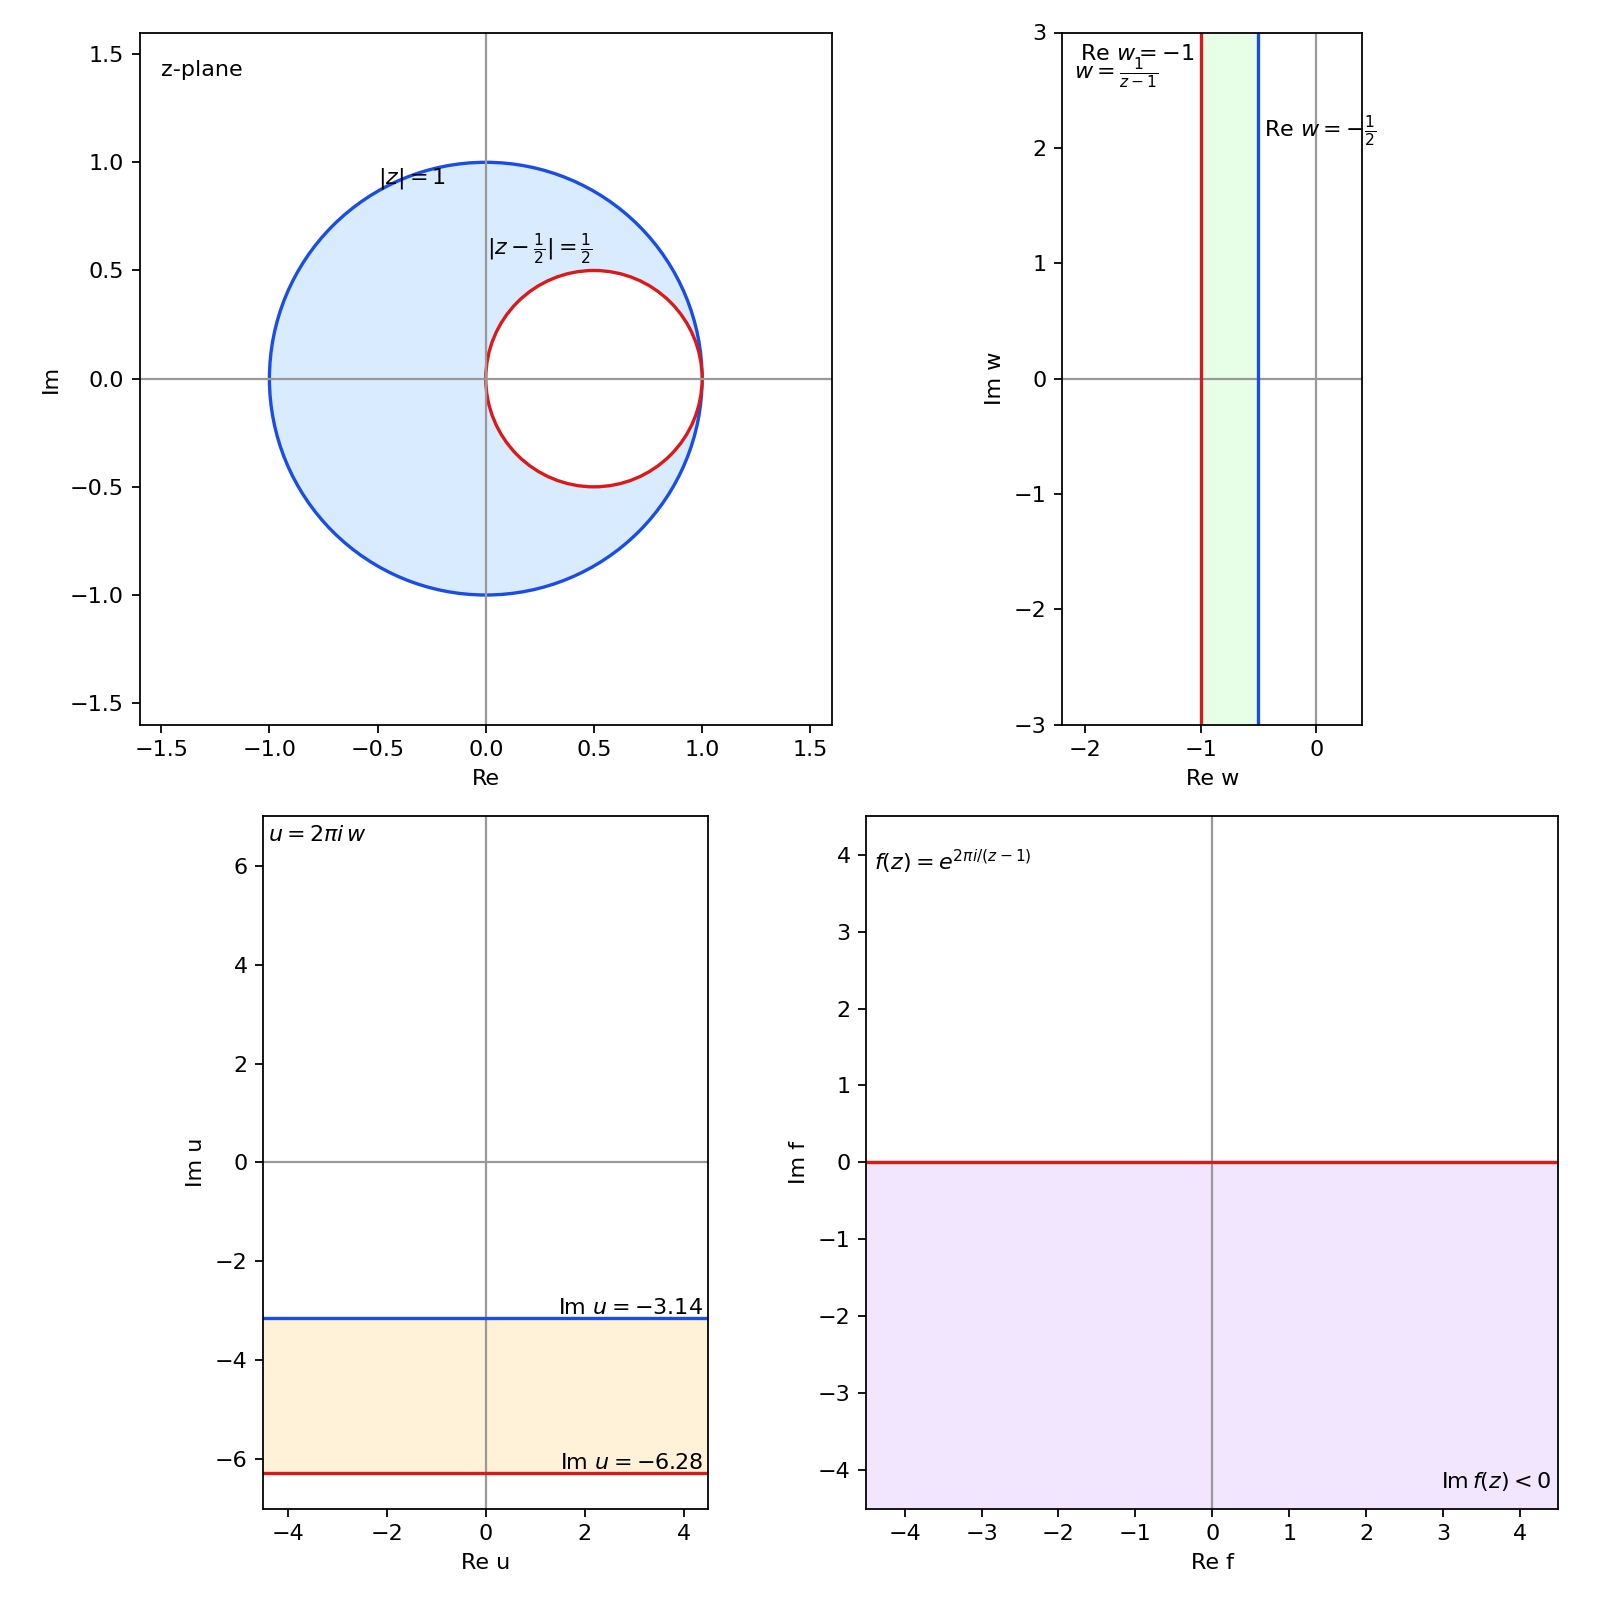
\includegraphics[scale=0.65]{conformal-mapping.png}
        \end{figure}
    \end{sol}
\end{exercise}

\section{Elementary Riemann Surfaces}
This is an optional section to introduce Riemann surfaces. We won't need this material, however.

The visualization of a function by means of the corresponding mapping is completely clear only when the mapping is one to one. If this is not the case, we can still give our imagination the necessary support by the introduction of generalized regions in which distinct points may have the same coordinates. In order to do this it is necessary to suppose that points which occupy the same place can be distinguished by other characteristics, for instance a tag or a color. Points with the same tag are considered to lie in the same \emph{sheet} or \emph{layer}.

This idea leads to the notion of a \emph{Riemann surface}, which is -- put simply -- a one-dimensional complex connected smooth manifold. For example, the Riemann sphere we have been dealing with all throughout this text is better known as $\CC\PP^1$, \emph{complex projective $1$-space}. With our construction, it is obvious that $\CC\PP^1$ is equivalent to a sphere, but this can be proven rigorously starting from its definition $$\CC\PP^1=\CC^2 \quotient \sim, \quad (z_1,z_2) \sim (z_1',z_2') \iff \dfrac{z_1}{z_1'}=\dfrac{z_2}{z_2'}.$$ Then $\CC\PP^1$ can be shown to be diffeomorphic to $S^2$. This requires familiarity with differential topology.

It is not our intention to give a rigorous definition of a Riemann surface; for our purposes it is sufficient to introduce it in a purely descriptive manner. The interested reader can follow up with a course on Riemannian geometry. For now, we content ourselves with some informally developed examples.

\begin{example}
    The simplest Riemann surface is connected with the mapping by a power $w=z^n$, where $n>1$ is an integer. We know that there is a one-to-one correspondence between each angle $(k-1)(2\pi/n)<\arg z<k(2\pi/n)$, $k=1,2,\dots,n$, and the whole $w$-plane except for the positive real axis. The image of each angle is thus obtained by performing a ``cut'' along the positive axis; this cut has an upper and lower ''edge.'' Corresponding to the $n$ angles in the $z$-plane we consider $n$ identical copies of the $w$-plane with the cut. They will be the ``sheets'' of the Riemann surface, and they are distinguished by a tag $k$ which serves to identify the corresponding angle. When $z$ moves in the plane, the point $w$ should be free to move on the Riemann surface. For this reason, we must attach the lower edge of the first sheet to the upper edge of the second, and so on. In the last step the lower edge of the $n$th sheet is attached to the upper edge of the first, completing the cycle. In a physical sense this is not possible without self-intersection, bu the idealized model shall be free from this discrepancy. The result of the construction is a Riemann surface whose points are in one-to-one correspondence with the points of the $z$-plane. What is more, this correspondence is continuous if continuity is defined in the sense suggested by the construction.

    The cut along the positive axis could be replaced by a cut along any simple arc from $0$ to $\infty$.

    The point $0$ is called a \emph{branch point} since it connects all the sheets. In general, if a point connects $h$ sheets, it is said to be a branch point of order $h-1$.
\end{example}

\begin{example}
    The Riemann surface corresponding to $w=e^z$ is of similar nature. In this case the function maps each parallel strip $(k-1)2\pi<y<k \cdot 2\pi$ onto a sheet with a cut along the positive axis. The sheets are attached to each other so that they form an endless screw. The origin will \textit{not} be a point of the Riemann surface, because $e^z$ is never zero.
\end{example}

\part{Complex Integration}
Having thoroughly studied the differentiable aspects of complex functions, we now turn to the study of integration. The theory of complex integration is one of the most beautiful and powerful parts of complex analysis, and it is the key to many important results in the field.

Many important properties of analytic functions are very difficult to prove without use of complex integration. And even if there do exist integration-free proofs, they are considerably more difficult.

We'll begin our exploration by building up some of the most important results on integrating analytic functions over various curves; this will ultimately lead to the powerful Cauchy Integral Formula. Following Ahlfors' philosophy, we will prove all theorems purely analytically. However, we must note that Cauchy's Integral Formula (and, frankly, all related results appearing beforehand) is a special case of Stokes' Theorem and the degree formula from differential topology. The reader who is well-acquainted with differential forms on smooth manifolds may have already derived Cauchy's Integral Formula as an exercise using these methods. In all honesty, we believe that the analytical arguments, particularly the ones that Ahlfors employs, are so simply beautiful that they should not be neglected. The interested reader can consult the appendix for a brief foray into differential topology, in which we quickly introduce differential forms, prove Stokes' Theorem, connect the analytical and topological notions of degree and winding number, and prove Cauchy's Integral Formula in this alternative manner.
\chapter{Fundamental Theorems}
\label{chap:fundamental-theorems}
As in the real case we distinguish between \emph{definite} and \emph{indefinite} integrals. An indefinite integral is a function whose derivative equals a given analytic function in a region; in many elementary cases indefinite integrals can be found by inversion of known derivation formulas. The definite integrals are taken over differentiable or piecewise differentiable arcs and are not limited to analytic functions. They can be defined by a limit process which mimics the definition of a real definite integral. Actually, we shall prefer to define complex definite integrals in terms of real integrals. This will save us from repeating existence proofs which are essentially the same as in the real case. Naturally, we presuppose that the reader is familiar with real integral calculus.

\section{Line Integrals}
The most immediate generalization of a real integral is to the definite integral of a complex function over a real interval. 

\begin{definition}[Line Integral]
If $f(t)=u(t)+iv(t)$ is a continuous function defined in an interval $(a,b)$, we set $$\int_{a}^{b}f(t)dt=\int_{a}^{b}u(t)dt+i\int_{a}^{b}v(t)dt.$$ This integral is called the \emph{line integral} of the function $f$ over the interval $(a,b)$.
\end{definition}

This integral has most of the properties of a real integral. In particular, if $c=\alpha+i\beta$ is a complex constant, then we obtain $$\int_{a}^{b} cf(t)dt=\int_{a}^{b}(\alpha u-\beta v)dt+i\int_{a}^{b}(\alpha v+\beta u)dt=c\int_{a}^{b} f(t)dt.$$ When $a \le b$, the fundamental inequality $$\left\abs{\int_{a}^{b} f(t)dt\right}\le \int_{a}^{b} \abs{f(t)}dt$$ holds for arbitrary complex $f(t)$. To see this we choose $c=e^{-i\theta}$ with a real $\theta$ and find that $$\Real\left[e^{-i\theta} \int_{a}^{b}f(t)dt\right]=\int_{a}^{b}\int_{a}^{b}\Real\left[e^{-i \theta}f(t)\right]dt \le \int_{a}^{b}\abs{f(t)}dt.$$ For $\theta=\arg \int_{a}^{b}f(t)dt$ the expression on the left reduces to the absolute value of the integral, and the desired inequality results. (Note: $\theta$ is not defined when $\int_{a}^{b} fdt=0$, but then there is nothing to prove.)

We now define a generalized line integral over a complex-valued arc, rather than a real interval.

\begin{definition}[Line Integral over an Arc]
    Let $\gamma$ be a piecewise differentiable arc with the equation $z=z(t)$, $a \le t \le b$. If the function $f(z)$ is defined and continuous on $\gamma$, then $f(z(t))$ is also continuous, and we define the \emph{line integral} of $f$ over $\gamma$ by $$\int_{\gamma}f(z)dz=\int_{a}^{b}f(z(t))z'(t)dt.$$
\end{definition}

In the right-hand side of the definition above, if $z'(t)$ is not continuous throughout, the interval of integration has to be subdivided in the obvious manner. Whenever a line integral over an arc $\gamma$ is considered, let it be tacitly understood that $\gamma$ is piecewise differentiable.

The most important property of the line integral is its invariance under a change of parameter. A change of parameter is determined by an increasing function $t=t(\tau)$ which maps an interval $\alpha \le \tau \le \beta$ diffeomorphically onto $a \le t \le b$; we assume that $t(\tau)$ is piecewise differentiable. By the rule for changing the variable of integration, we have $$\int_{a}^{b} f(z(t))z'(t)dt=\int_{\alpha}^{\beta} f(z(t(\tau)))z'(t(\tau))t'(\tau)d\tau.$$ But $z'(t(\tau))t'(\tau)$ is the derivative of $z \circ t$ with respect to $\tau$, and hence the integral has the same value whether $\gamma$ be represented by the equation $z=z(t)$ or by the equation $z=z(t(\tau))$.

Recall that we defined the \emph{opposite} arc $-\gamma$ by the equation $z=z(-t)$, $-b \le t \le -a$. We have thus $$\int_{-\gamma} f(z)dz = -\int_{-b}^{a}f(z(-t))(-z'(-t))dt=\int_{b}^{a}f(z(t))z'(t)dt=-\int_{\gamma}f(z)dz.$$ This shows that the line integral over an opposite arc is the negative of the line integral over the original arc.

The line integral also has a very obvious additive property. It is quite clear what is meant by subdividing an arc $\gamma$ into a finite number of subarcs. A subdivision can be indicated by a symbolic equation $$\gamma=\gamma_1+\gamma_2+\cdots+\gamma_n,$$ where each $\gamma_i$ is a piecewise differentiable arc. The corresponding line integrals then satisfy the relation $$\int_{\gamma}f(z)dz=\sum_{i=1}^{n}\int_{\gamma_i}f(z)dz.$$ Finally, the integral over a closed curve is also invariant under a shift of parameter. The old and the new initial point determine two subarcs $\gamma_1,\gamma_2$, and the invariance follows from the fact that the integral over $\gamma_1+\gamma_2$ is the same as the integral over $\gamma_2+\gamma_1$.

In addition, we can also consider line integrals with respect to $\overline{z}$. The most convenient definition is by double conjugation: $$\int_{\gamma} f d\overline{z}=\overline{\int_{\gamma} \overline{f} dz}.$$ Using this notation, line integrals with respect to $x$ and $y$ can be introduced. Let $\gamma$ be parametrized as $z(t)=x(t)+iy(t)$. Then $z'(t)=x'(t)+iy'(t)$ (remember, $x$ and $y$ are just real functions of a real variable, so there are no partial derivatives to worry about). Hence,
\begin{align*}
\int_{\gamma} f \overline{dz} &=\overline{\int_{\gamma} \overline{f} dz} \\
&=\overline{\int_{a}^{b} \overline{f(z(t))} z'(t) dt} \\
&=\int_{a}^{b} f(z(t)) \overline{z'(t)} dt \\
&=\int_{a}^{b} f(z(t)) \left[x'(t)-iy'(t)\right]dt.
\end{align*}
Setting $$\int_{\gamma} fdx=\int_{a}^{b}f(z(t))x'(t)dt \quad \text{and} \quad \int_{\gamma} fdy=\int_{a}^{b}f(z(t))y'(t)dt,$$ we obtain the relations
\begin{align*}
\int_{\gamma} f dx &=\dfrac{1}{2}\left(\int_{\gamma} f dz + \int_{\gamma} f \overline{dz}\right), \\
\int_{\gamma} f dy &=\dfrac{1}{2i}\left(\int_{\gamma} f dz - \int_{\gamma} f \overline{dz}\right).
\end{align*}
With $f=u+iv$ we find that the line integral can also be written in the form $$\int_{\gamma} (u dx-v dy)+i\int_{\gamma} (u dx+v dy)$$ which separates the real and imaginary parts.

An essentially different line integral is obtained by integration with respect to \emph{arc length}. Two notations are in common use, and the definition is $$\int_{\gamma} f ds=\int_{\gamma} f \abs{dz}=\int_{a}^{b} f(z(t)) \abs{z'(t)} dt.$$ This integral is again independent of the choice of parameter. We have $$\int_{-\gamma} f \abs{dz}=\int_{-b}^{-a} f(z(-t)) \abs{-z'(-t)} dt=\int_{a}^{b} f(z(t)) \abs{z'(t)} dt,$$ and again, by the change of parameter $t=-\tau$, we find that $$\int_{-\gamma}f\abs{dz}=-\int_{b}^{a} f(z(t)) \abs{z'(t)} dt=\int_{\gamma} f \abs{dz}.$$ The additive property is also valid, and the inequality $$\left\abs{\int_{\gamma} f dz\right}\le \int_{\gamma} \abs{f} \abs{dz}$$ holds.

For $f=1$ the arc length integral reduces to $\int_{\gamma} \abs{dz}$, which is by definition the \emph{length} of the curve $\gamma$.

\begin{example}[Circumference of a circle]
As an exercise in overkill, let us use the theory we have developed of line integrals to compute the length of a circle. As usual, parameterize a circle $C$ with center $a$ and radius $\rho$ by $z=z(t)=a+\rho e^{it}$, $0 \le t \le 2\pi$ (we can leave $2\pi$ out to make the parameterization bijective, but this has no consequence on the integral). Then the circumference is simply the line integral of the constant function $f=1$ over the entire circle, so we get $$\int_{C}dz=\int_{0}^{2\pi}\abs{z'(t)}dt=\int_{0}^{2\pi}\abs{i\rho e^{it}}dt=\int_{0}^{2\pi}\rho dt=2\pi\rho,$$ as expected.
\end{example}

\section{Line Integrals as Functions of Arcs}

General line integrals of the form $\int_{\gamma} p dx+q dy$ are often studied as functions (or \emph{functionals}) of the arc $\gamma$. It is then assumed that $p$ and $q$ are defined and continuous in a region $\Omega$ and that $\gamma$ is free to vary in $\Omega$.

An important class of integrals is characterized by the property that the integral over an arc depends only on its endpoints. In other words, if $\gamma_1$ and $\gamma_2$ have the same initial point and the same end point, we require that $$\int_{\gamma_1} p dx+q dy=\int_{\gamma_2} p dx+q dy.$$ Why? Well, to say that an integral depends only on the endpoints is equivalent to saying that the integral over any closed curve is zero. Indeed, if $\gamma$ is a closed curve, then $\gamma$ and $-\gamma$ have the same endpoints, and if the integral depends only on the end points, then $$\int_{\gamma}=\int_{-\gamma}=-\int_{\gamma},$$ giving $\int_{\gamma}=0$. Conversely, if $\gamma_1$ and $\gamma_2$ have the same endpoints, then $\gamma_1-\gamma_2$ is a closed curve, and if the integral over any closed curve vanishes, it follows by the additive property of the integral that $\int_{\gamma_1}=\int_{\gamma_2}$.

The following theorem, our first major one on integration, gives a necessary and sufficient condition for the integral to depend only on the endpoints.

\begin{theorem}
\label{thm:exact-differential}
The line integral $\int_{\gamma} p dx+q dy$, defined in $\Omega$, depends only on the endpoints of $\gamma$ if and only if there exists a function $U(x,y)$ defined in the region $\Omega$ such that $$p=\frac{\partial U}{\partial x}, \quad q=\frac{\partial U}{\partial y}$$ in $\Omega$.
\end{theorem}

\begin{proof}
The sufficiency follows at once, for if the condition is fulfilled we can write, with the usual notations,
\begin{align*}
    \int_{\gamma} p dx+q dy &= \int_{a}^{b} \frac{\partial U}{\partial x} x'(t) + \frac{\partial U}{\partial y} y'(t) dt \\
    &= \int_{a}^{b} \dfrac{d}{dt}U(x(t),y(t))dt \\
    &=U(x(b),y(b))-U(x(a),y(a)),
\end{align*}
and the value of this difference, of course, only depends on the endpoints $x(a)+iy(a)$ and $x(b)+iy(b)$.

To prove the necessity we choose a fixed point $(x_0,y_0) \in \Omega$, join it to $(x,y)$ by a polygon $\gamma$, contained in $\Omega$, whose sides are parallel to the coordinate axes, and define a function by $$U(x,y)=\int_{\gamma} p dx+q dy.$$ Since the integral depends only on the end points, the function is well defined. Moreover, if we choose the last segment of $\gamma$ horizontal, we can keep $\gamma$ constant and let $x$ vary without changing the other segments. On the last segment, we can choose $x$ for paramter and obtain $$U(x,y)=\int^{x}p(x,y)dx+C$$ for some constant $C$, the lower limit of the integral being irrelevant. From this expression it follows at once that $\partial U/\partial X=p$. In the same way, by choosing the last segment vertical, we can show that $\partial U/\partial y=q$. Thus, the function $U$ exists and satisfies the required conditions.
\end{proof}

If you have studied differential geometry, you may recognize the expression $dU=(\partial U/\partial X)dx+(\partial U/\partial y)dy$ as an \emph{exact differential form}; the function $U$ is called the \emph{exterior derivative} of the form $p dx+q dy$. If a differential form $p dx+q dy$ is exact, then the function $U$ is uniquely determined, up to a constant.

In the case of complex functions, when is $f(z)dz=f(z)dx+if(z)dy$ an exact differential form? According to the definition there must exist a function $F(z)$ in $\Omega$ with the partial derivatives
\begin{align*}
\frac{\partial F}{\partial x} &= f(z) \\
\frac{\partial F}{\partial y} &= if(z).
\end{align*}
If this is so, then $F(z)$ fulfills the Cauchy-Riemann equation $$\dfrac{\partial F}{\partial x}=-i\dfrac{\partial F}{\partial y},$$ and hence $f(z)$ is analytic in $\Omega$. Thus, we have the following corollary:
\begin{corollary}
\label{cor:line-integral-endpoints}
The integral $\int_{\gamma} fdz$, with continuous $f$, depends only on the endpoints of $\gamma$ if and only if $f$ is the derivative of an analytic function in the region $\Omega$ containing $\gamma$.
\end{corollary}
Under these circumstances we shall prove later that $f(z)$ is itself analytic.

\begin{example}
As an immediate application of the Corollary \ref{cor:line-integral-endpoints}, we find that $$\int_{\gamma}(z-a)^ndz=0$$ for all closed curves $\gamma$, provided that the integer $n \ge 0$. In fact, $(z-a)^n$ is the derivative of $(z-a)^{n+1}/(n+1)$, which is analytic in the whole plane. If $n$ is negative, but not equal to $-1$, the same result holds for all closed curves $\gamma$ which do not pass through $a$. And for $n=-1$, the result is not necessarily true, for consider a circle $C$ with center $a$, represented by the equation $z=a+\rho e^{it}$, $0 \le t \le 2\pi$. We obtain $$\int_{C}\dfrac{dz}{z-a}=\int_{0}^{2\pi}\dfrac{ipe^{it}}{pe^{it}}dt=\int_{0}^{2\pi}idt=2\pi i.$$ This result shows that it is impossible to define a single-valued branch of $\log(z-a)$ in an annulus $\rho_1<\abs{z-a}<\rho_2$. On the other hand, if the closed curve is contained in a half plane which does not contain $a$, the integral vanishes, for in such a half plane a single-valued and analytic branch of $\log(z-a)$ can be defined.
\end{example}

\begin{exercise}
    Compute the following integrals.
    \begin{enumerate}
    \item[(a)] $\int_{\gamma} x dz,$ where $\gamma$ is the directed line segment from $0$ to $1+i$.
    \item[(b)] $\int_{\abs{z}=r} x dz$ for the positive sense of the circle.
    \item[(c)] $\int_{\abs{z}=2}\dfrac{dz}{z^2-1}$ for the positive sense of the circle.
    \end{enumerate}

    \begin{sol}
    $ $
    \begin{enumerate}
    \item[(a)] The answer is $\boxed{\frac{1}{2}+\frac{1}{2}i}$.
    
    Parametrize $\gamma$ as $z(t)=(1+i)t=t+it$, $0 \le t \le 1$. Then \begin{align*}
    \int_{\gamma} x dz &=\int_{0}^{1} t(1+i)dt \\
    &=\int_{0}^{1}t dt+i\int_{0}^{1}t dt \\
    &=\left[\frac{t^2}{2}\right]_{0}^{1}+i\left[\frac{t^2}{2}\right]_{0}^{1} \\
    &=\frac{1}{2}+\frac{1}{2}i.
    \end{align*}
    \item[(b)] The answer is $\boxed{\pi i r^2}$.
    We'll show two different approaches to this problem. First, parameterize the circle as $z(t)=re^{it}$ for $0 \le t \le 2\pi$; then \begin{align*}
    \int_{\abs{z}=r} x dz &=\int_{0}^{2\pi} r\cos(t) i r e^{it} dt \\
    &=i r^2 \int_{0}^{2\pi} \cos(t)e^{it} dt \\
    &=\dfrac{ir^2}{2} \int_{0}^{2\pi}(e^{2it}+1)dt \\
    &=\dfrac{ir^2}{2}\left[t\right]_{0}^{2\pi} \\
    &=\dfrac{2\pi ir^2}{2} \\
    &=\pi i r^2,
    \end{align*}

    where we used the fact that $\int_{0}^{2\pi} e^{nit} dt=0$ for any $n \in \ZZ$.

    On the other hand, we can employ a slicker idea: observe that $x=\frac{1}{2}\left(z+\overline{z}\right)=\frac{1}{2}\left(z+\frac{r^2}{z}\right)$ on the circle $\abs{z}=r$. Note that $\int_{\abs{z}=r}zdz=0$ as $z$ is the derivative of an analytic function. Hence, $$\int_{\abs{z}=r} x dz=\dfrac{r^2}{2}\int_{\abs{z}=r}\dfrac{dz}{z}=\dfrac{r^2}{2}\cdot 2\pi i=\pi i r^2,$$ where we used the fact from the text that $\int_{\abs{z}=r} \frac{dz}{z}=2\pi i$.
    \item[(c)] The answer is $\boxed{0}$. Via partial fraction decomposition, write $$\dfrac{1}{z^2-1}=\dfrac{1/2}{z-1}-\dfrac{1/2}{z+1}.$$ Hence, $$\int_{\abs{z}=2}\dfrac{dz}{z^2-1}=\dfrac{1}{2}\left(\int_{\abs{z}=2}\dfrac{dz}{z-1}-\int_{\abs{z}=2}\dfrac{dz}{z+1}\right)=0.$$
    \end{enumerate}
    \end{sol}
\end{exercise}

\begin{exercise}
Suppose that $f(z)$ is $C^1$ analytic on a closed curve $\gamma$ (i.e., $f$ is analytic in a region containing $\gamma$). Show that $$\int_{\gamma}\overline{f(z)}f'(z)dz$$ is purely imaginary.

\begin{sol}
    There a number of ways to solve this problem, some slicker than others. We'll use a bit more computational method expressing the complex integral in terms of real differential forms, which the reader is probably more familiar with.

    Write $f(z)=u(x,y)+iv(x,y)$. Then \begin{align*}
    \Real \int_{\gamma}\overline{f(z)}f'(z)dz &= \int_{\gamma}(u-iv)\left(\frac{\partial u}{\partial x}+i\dfrac{\partial v}{\partial x}\right)\left(dx+idy\right) \\
    &=\Real \int_{\gamma}\left[u \cdot \dfrac{\partial u}{\partial x}+v \cdot \dfrac{\partial v}{\partial x}+i\left(u \cdot \dfrac{\partial v}{\partial x}-v \cdot \dfrac{\partial u}{\partial x}\right)\right](dx+idy) \\
    &=\int_{\gamma}\left(u \cdot \dfrac{\partial u}{\partial x}v \cdot \dfrac{\partial v}{\partial x}\right)dx+\left(-u \cdot \dfrac{\partial v}{\partial x}+v \cdot \dfrac{\partial u}{\partial x}\right)dy \\
    &=\int_{\gamma} \left(u \cdot \dfrac{\partial u}{\partial x}v \cdot \dfrac{\partial v}{\partial x}\right)dx+\left(u \cdot \dfrac{\partial u}{\partial y}+v \cdot \dfrac{\partial v}{\partial y}\right)dy & \text{Cauchy-Riemann} \\
    &=\int_{\gamma}d(u^2+v^2) \\
    &=0,
    \end{align*}
    as the integral of an exact differential form over a closed curve is zero. Hence, the real part of the given integral is zero, and thus the integral is purely imaginary.
\end{sol}
\end{exercise}

\section{Cauchy's Theorem for a Rectangle}
As we noted in the introduction to this chapter, Cauchy's Theorem falls out of Stokes' Theorem once that more general case is known. However, in the interest of not using a sledgehammer to crack a nut, let us begin by building up our theory in a purely analytical way.

First, consider a rectangle $R$ defined by inequalities $a \leq x \leq b$, $c \leq y \leq d$. Its perimeter can be considered as a simple closed curve consisting of four line segments whose direction we choose so that $R$ lies to the left of the directed segments. The order of the vertices is thus $(a,c)$, $(b,c)$, $(b,d)$, $(a,d)$, and back to $(a,c)$. We denote the perimeter of $R$ by $\partial R$ and refer to it as the \emph{boundary curve} or \emph{contour} of $R$; note that this is standard notation from topology.

We emphasize that $R$ is chosen as a closed point set and, hence, is not a region. In the theorem that follows we consider a function which is analytic on the rectangle $R$. We recall that such a function is by definition defined and analytic in a region which contains $R$.

The following is a preliminary version of \emph{Cauchy's Theorem}:
\begin{theorem}[Cauchy]
\label{thm:cauchy-rectangle}
If the function $f(z)$ is analytic on $R$, then $$\int_{\partial R} f(z)dz=0.$$
\end{theorem}

\begin{proof}
The proof is quite beautiful and based on the method of bisection. Let us introduce the notation $$\eta(R)=\int_{\partial R} f(z)dz,$$ which we will also use for any rectangle contained in the given one. If $R$ is divided into four congruent rectangles $R^{(1)}, R^{(2)}, R^{(3)}, R^{(4)}$, then by the linearity of the integral and the observation that the integrals over the common sides cancel each other, we have $$\eta(R)=\sum_{j=1}^{4}\eta(R^{(j)}).$$

\begin{figure}[h]
\caption{Bisection of rectangle.}
\centering
\begin{asy}
unitsize(2.5cm);

// Define the rectangle
real a = 3;
real b = 2;

// Rectangle corners
pair A = (0,0);
pair B = (a,0);
pair C = (a,b);
pair D = (0,b);

// Midpoints for bisection
pair M1 = (a/2, 0);    // bottom midpoint
pair M2 = (a, b/2);    // right midpoint  
pair M3 = (a/2, b);    // top midpoint
pair M4 = (0, b/2);    // left midpoint
pair O = (a/2, b/2);   // center point

// Draw outer rectangle with thick boundary
draw(A--B--C--D--cycle, linewidth(2bp));

// Draw bisection lines (dashed)
draw(M1--M3, dashed + gray(0.5));
draw(M4--M2, dashed + gray(0.5));

// Function to draw arrow next to a segment
void drawArrowNearSegment(pair start, pair end, real offset=0.1, real arrowsize=3) {
    pair mid = 0.5*(start + end);
    pair dir = unit(end - start);
    pair perp = rotate(90)*dir;  // perpendicular direction
    pair arrowStart = mid + offset*perp;
    pair arrowEnd = arrowStart + 0.2*dir;
    draw(arrowStart--arrowEnd, Arrow(size=arrowsize));
}

// Draw arrows for internal horizontal segments only (not outer boundary)
drawArrowNearSegment(A, M1, -0.08);    // bottom-left horizontal
drawArrowNearSegment(M1, B, -0.08);    // bottom-right horizontal
drawArrowNearSegment(D, M3, 0.08);     // top-left horizontal (leftward)
drawArrowNearSegment(M3, C, 0.08);     // top-right horizontal (leftward)

// Draw arrows for internal vertical segments only (not outer boundary)
drawArrowNearSegment(D, M4, -0.08);    // left-top vertical (downward)
drawArrowNearSegment(M4, A, -0.08);    // left-bottom vertical (downward)
drawArrowNearSegment(B, M2, 0.08);     // right-bottom vertical (upward)
drawArrowNearSegment(M2, C, 0.08);     // right-top vertical (upward)

// Draw clearly opposing arrows for center cross segments to show cancellation
// Horizontal center line - arrows on opposite sides pointing in opposite directions
drawArrowNearSegment(M4, O, -0.08);    // left half: rightward, below line
drawArrowNearSegment(O, M2, -0.08);    // right half: rightward, below line
drawArrowNearSegment(O, M4, 0.08);     // left half: leftward, above line
drawArrowNearSegment(M2, O, 0.08);     // right half: leftward, above line

// Vertical center line - arrows on opposite sides pointing in opposite directions
drawArrowNearSegment(M1, O, -0.08);    // bottom half: upward, left of line
drawArrowNearSegment(O, M3, -0.08);    // top half: upward, left of line
drawArrowNearSegment(O, M1, 0.08);     // bottom half: downward, right of line
drawArrowNearSegment(M3, O, 0.08);     // top half: downward, right of line

// Add rectangle labels
label("$R^{(1)}$", (a/4, b/4));
label("$R^{(2)}$", (3*a/4, b/4));
label("$R^{(3)}$", (3*a/4, 3*b/4));
label("$R^{(4)}$", (a/4, 3*b/4));

// Add corner labels
label("$(a,c)$", A, SW);
label("$(b,c)$", B, SE);
label("$(b,d)$", C, NE);
label("$(a,d)$", D, NW);
\end{asy}
\end{figure}

It follows that at least one of the rectangle $R^{(k)}$, $1 \le k \le 4$, must satisfy the condition $$\abs{\eta(R^{(k)})} \ge \dfrac{1}{4}\abs{\eta(R)}.$$ If we continue this process, we can find a sequence of rectangles $R_1 \supset R_2 \supset \cdots \supset R_n \supset \cdots$ such that $$\abs{\eta(R_n)} \ge 4^{-n}\abs{\eta(R)}.$$ The rectangles converge to a point $z^* \in R$ in the sense that $R_n$ will be contained in a prescribed neighborhood $\abs{z-z^*}<\delta=B_{\delta}(z^*)$ as soon as $n$ is sufficiently large. First of all, we choose $\delta$ so small that $f(z)$ is defined and analytic in $\abs{z-z^*}<\delta$. Secondly, if $\eps>0$ is given, we can choose $\delta$ so that $$\left\abs{\dfrac{f(z)-f(z^*)}{z-z^*}-f'(z^*)\right} \le \eps$$ or $$\abs{f(z)-f(z^*)-(z-z^*)f'(z^*)}\le \eps\abs{z-z^*}$$ for all $z$ in the neighborhood $B_{\delta}(z^*)$. We assume that $\delta$ satisfies both conditions and that $R_n$ is contained in $B_{\delta}(z^*)$.

We make now the observation that
\begin{align*}
\int_{\partial(R_n)}dz &=0, \\
\int_{\partial(R_n)}zdz &=0,
\end{align*}
as both $dz$ and $zdz$ are exact differentials and $\partial(R_n)$ is a closed curve. By virtue of these equations, and noting that $z^*$ is a fixed constant, we are able to write
\begin{align*}
\eta(R_n) &= \int_{\partial(R_n)} f(z)dz \\
&=\int_{\partial(R_n)}\left[f(z)-f(z^*)-(z-z^*)f'(z^*)\right]dz,
\end{align*}
and it follows that $$\abs{\eta(R_n)} \le \eps \int_{\partial(R_n)}\abs{z-z^*} \cdot \abs{dz}.$$ In this last integral $\abs{z-z^*}$ is at most equal to the diagonal $d_n$ of $R_n$. If $L_n$ denotes the length of the perimeter of $R_n$, the integral is hence at most $d_nL_n$. But if $d$ and $L$ are the corresponding quantities for the original rectangle $R$, then it is clear that $d_n=2^{-n}d$ and $L_n=2^{-n}L$ by construction. Hence, $$\abs{\eta(R)} \le 4^{n}\abs{\eta(R_n)} \le 4^{n} \cdot 4^{-n}dL\eps=dL\eps.$$ Since $\eps$ is arbitrary, we can only have $\abs{\eta(R)}=0$, and the theorem is proved.
\end{proof}

It turns out that the hypothesis in Theorem \ref{thm:cauchy-rectangle} can be weakened considerably. We shall prove at once the stronger theorem which will find very important use.

\begin{theorem}
\label{thm:cauchy-rectangle-stronger}
Let $f(z)$ be analytic on the set $R'$ obtained from a rectangle $R$ by omitting a finite number of interior points $\zeta_j$. If it is true that $$\lim_{z \rightarrow \zeta_j} (z-\zeta_j)f(z)=0$$ for all $j$, then $$\int_{\partial R} f(Z)dz=0.$$
\end{theorem}
\begin{proof}
It is sufficient to consider the case of a single exceptional point $\zeta$, for evidently $R$ can be divided into smaller rectangles which contain at most one $\zeta_j$.

We divide $R$ into nine rectangles, as shown in the figure below, and apply Theorem \ref{thm:cauchy-rectangle} to all but the rectangle $R_0$ in the center.

\begin{figure}[h]
\caption{Bisection of a rectangle into nine parts.}
\centering
\begin{asy}
import math;
size(300);

// Define the large rectangle dimensions
real width = 6;
real height = 4;

// Draw the large rectangle
draw((0,0)--(width,0)--(width,height)--(0,height)--cycle, linewidth(1.5));

// Define grid divisions (3x3 grid)
real dx = width/3;
real dy = height/3;

// Draw vertical grid lines
for(int i = 1; i <= 2; ++i) {
    // Dashed lines extending to outer edges
    draw((i*dx, 0)--(i*dx, dy), linewidth(1) + dashed);
    draw((i*dx, 2*dy)--(i*dx, height), linewidth(1) + dashed);
    
    // Solid line through the central rectangle
    draw((i*dx, dy)--(i*dx, 2*dy), linewidth(1));
}

// Draw horizontal grid lines
for(int i = 1; i <= 2; ++i) {
    // Dashed lines extending to outer edges
    draw((0, i*dy)--(dx, i*dy), linewidth(1) + dashed);
    draw((2*dx, i*dy)--(width, i*dy), linewidth(1) + dashed);
    
    // Solid line through the central rectangle
    draw((dx, i*dy)--(2*dx, i*dy), linewidth(1));
}

// Mark the point ζ in the central rectangle
pair zeta = (1.5*dx, 1.5*dy);
dot(zeta, linewidth(4));
label("$\zeta$", zeta, NE, fontsize(12));

\end{asy}
\end{figure}
This gives $$\int_{\partial R} fdz=\int_{\partial R_0} f dz.$$ By hypothesis, if $\eps>0$ we can choose the rectangle $R_0$ so small that $$\abs{f(z)} \le \dfrac{\eps}{\abs{z-\zeta}}$$ on $\partial R_0$. Hence, $$\left\abs{\int_{\partial R} f dz\right} \le \eps \int_{\partial R_0} \dfrac{\abs{dz}}{\abs{z-\zeta}}.$$ If we assume, as we may, that $R_0$ is a square of center $\zeta$ with side length $s$, then by elementary estimates, we find that
\begin{align*}
\int_{\partial R_0} \dfrac{\abs{dz}}{\abs{z-\zeta}} &<\int_{\partial R_0} \dfrac{\abs{dz}}{\inf_{z \in \partial R_0}(\abs{z-\zeta})} \\
&=2\int_{\partial R_0} \dfrac{\abs{dz}}{s} \\
&=2 \cdot 4s \cdot \dfrac{1}{s} \\
&=8.
\end{align*}
Thus, we obtain $$\left\abs{\int_{\partial R} fdz\right}<8\eps,$$ and -- again -- since $\eps$ is arbitrary, the theorem follows.
\end{proof}

We observe that the hypothesis of the theorem is certainly fulfilled if $f(z)$ is analytics and \emph{bounded} on $R'$.

\section{Cauchy's Theorem in a Circular Disk}
It is not true that the integral of an analytic function over a closed curve is always zero. Indeed, we have found that $$\int_{C} \dfrac{dz}{z-a}=2\pi i$$ where $C$ is a circle about $a$. In order to make sure that the integral vanishes, it is necessary to make a special assumption concerning the region $\Omega$ in which $f(z)$ is known to be analytic and to which the curve $\gamma$ is restricted. We are not yet in a position to formulate this condition, and for this reason we must restrict attention to a very special case. In what follows we assume that $\Omega$ is an open circular disk $\abs{z-z_0}<\rho$ to be denoted by $\Delta$.

\begin{theorem}
\label{thm:cauchy-disk}
If $f(z)$ is analytic in an open disk $\Delta$, then $$\int_{\gamma} f(z)dz=0$$ for every closed curve $\gamma$ in $\Delta$.
\end{theorem}
\begin{proof}
The proof is a repetition of the argument used in proving the second half of Theorem \ref{thm:exact-differential}. We define a function $F(z)$ by $$F(z)=\int_{\sigma} f dz$$ where $\sigma$ consists of the horizontal line segment from the center $(x_0,y_0)$ to $(x, y_0)$ and the vertical segment from $(x,y_0)$ to $(x,y)$; it is immediately seen that $\partial F/\partial y=if(z)$. On the other hand, $\sigma$ can be replaced by a path consisting of vertical segment followed by a horizontal segment. By Theorem \ref{thm:cauchy-rectangle}, this choice defines the same function $F(z)$ (since the signed sum of the integrals over both paths is zero). Hence, $\partial F/\partial x=f(z)$, and $F(z)$ is analytic in $\Delta$ with the derivative $f(z)$, making $f(z)dz$ an exact differential form.
\end{proof}

Clearly, the same proof would go through for any region with contains the rectangle with opposite vertices $z_0$ and $z$ as soon as it contains $z$, such as a half plane, or the inside of an ellipse. Howeever, this method does ot generalize to all types of regions.

As for the case of a rectangle, we may weaken the hypothesis.
\begin{theorem}
let $f(z)$ be analytic in the region $\Delta'$ obtained by omitting a finite number of points $\zeta_j$ from the disk $\Delta$. If it is true that $$\lim_{z \rightarrow \zeta_j} (z-\zeta_j)f(z)=0$$ for all $j$, then $$\int_{\gamma} f(z)dz=0$$ for every closed curve $\gamma$ in $\Delta'$.
\end{theorem}
\begin{proof}
The proof must be modified, for we cannot let $\sigma$ pass through the exceptional points. Assume first that no $\zeta_j$ lies on the lines $x=x_0$ and $y=y_0$. It is then possible to avoid the exceptional points by letting $\sigma$ consist of three segments, as shown in the figure below.

\begin{figure}[h]
\centering
\begin{asy}
size(8cm);

// Define the circle
pair center = (0, 0);
real radius = 2;
draw(circle(center, radius));

// Label the center
label("$(x_0, y_0)$", center, S);
dot(center);

// Define point z inside the circle (upper right)
pair z = (1.0, 0.8);
dot(z);
label("$z$", z, NE);

// Define exceptional point ζ between center and z
pair zeta = (0.4, 0.3);
dot(zeta, linewidth(3));
label("$\zeta$", zeta, SW);

// Draw the three-segment path from center to z avoiding zeta
// Segment 1: horizontal right from center
pair p1 = (zeta.x + 0.2, center.y);  // go right past zeta's x-coordinate
draw(center--p1, linewidth(1.2));

// Segment 2: vertical up 
pair p2 = (p1.x, z.y);  // go up to z's y-coordinate
draw(p1--p2, linewidth(1.2));

// Segment 3: horizontal right to z
draw(p2--z, linewidth(1.2));

// Draw the dashed alternative path (vertical, horizontal, vertical)
// Segment 1: vertical up from center
pair q1 = (center.x, zeta.y + 0.15);  // go up past zeta's y-coordinate
draw(center--q1, dashed + linewidth(1.0));

// Segment 2: horizontal right (crossing the solid path)
pair q2 = (z.x, q1.y);  // go right to z's x-coordinate
draw(q1--q2, dashed + linewidth(1.0));

// Segment 3: vertical down to z
draw(q2--z, dashed + linewidth(1.0));

\end{asy}
\end{figure}

By an obvious application of Theorem \ref{thm:cauchy-rectangle-stronger}, we find that the value of $F(z)$ is independent of the choice of the middle segment; moreover, the last segment can be either vertical or horizontal. We conclude as before that $F(z)$ is an indefinite integral of $f(z)$, and the theorem follows.

In case there are exceptional points on the lines $x=x_0$ and $y=y_0$, the reader will easily convince himself that a similar proof can be carried out, provided we use four line segments in the place of three.
\end{proof}
\chapter{Cauchy's Integral Formula}
\label{chap:cauchy-integral-formula}
Through a very simple application of Cauchy's theorem it becomes possible to represent an analytic function $f(z)$ as a line integral in which the variable $z$ centers as a parameter. This representation, known as \textit{Cauchy's Integral Formula}, has numerous important applications, not just in complex analysis, but also in physics and electrical engineering. Above all, it enables us to study the local properties of an analytic function in great detail.

As we declared at the beginning of this part on complex integration, we will prove Cauchy's Integral Formula purely analytically. That is, we will define winding number as an analytical, rather than a topological, quantity. For completeness, and to illustrate the connection between the two definitions, the Appendix, we will include a full topological proof of this quintessential theorem.

\section{Winding Number}
Central to many questions in function theory and physics (particularly string theory) is the notion of a curve winding around a point not on it. let us make this idea precise, inspired by the following lemma:
\begin{lemma}
If the piecewise differentiable closed curve $\gamma$ does not pass through the point $a$, then the value of the integral $$\int_{\gamma} \dfrac{dz}{z-a}$$ is a multiple of $2\pi i$.
\end{lemma}
\begin{proof}
This lemma may seem trivial, for we can write $$\int_{\gamma}\dfrac{dz}{z-a}=\int_{\gamma} d(\log(z-a))=\int_{\gamma}d(\log \abs{z-a})+i\int_{\gamma}d(\arg(z-a)).$$ When $z$ describes a closed durve, $\log\abs{z-a}$ returns to its intial value and $\arg(z-a)$ increases or decreases by a multiple of $2\pi$. This would seem to imply the lemma, but more careful thought shows that the reasoning is of no value unless we define $\arg(z-a)$ in a unique way. We could do this, but there is an easier way to proceed.

The simplest proof is computational, exploiting the theory of first-order ordinary differential equations. If the equation of $\gamma$ is $z=z(t)$, $\alpha \le t \le \beta$, let us consider the function $$h(t)=\int_{\alpha}^{t}\dfrac{z'(t)}{z(t)-a}dt.$$ It is defined and continuous on the closed interval $[\alpha, \beta]$, and it has the derivative $$h'(t)=\dfrac{z'(t)}{z(t)-a}$$ whenever $z'(t)$ is continuous. From this equation it follows that the derivative of $e^{-h(t)}(z(t)-a)$ is $$e^{-h(t)} \cdot z'(t)-h'(t)e^{-h(t)}(z(t)-a)=e^{-h(t)} \cdot z'(t)-e^{-h(t)} \cdot z'(t)=0$$ except perhaps at a finite number of points, and since this function is continuous it must reduce to a constant.

With the initial condition $h(\alpha)=0$, we solve the differential equation to get $$e^{h(t)}=\dfrac{z(t)-a}{z(\alpha)-a}.$$ Since $z(\beta)=z(\alpha)$ we obtain $e^{h(\beta)}=1$, and therefore $h(\beta)$ must be a multiple of $2\pi i$. This proves the lemma.
\end{proof}

Motivated by this fact, we can now precisely define the winding number of a point with respect to a curve.

\begin{definition}
Given a curve $\gamma$ and a point $a$ not on it, the \emph{winding number} of $\gamma$ with respect to $a$, denoted by $W(\gamma, a)$, is defined as the integer $$W(\gamma, a)=\frac{1}{2\pi i}\int_{\gamma} \dfrac{dz}{z-a}.$$
\end{definition}

It is clear that $W(-\gamma, a)=-W(\gamma, a)$, and the following property is an immediate consequence of \ref{thm:cauchy-disk}:

\textit{if $\gamma$ lies inside of a circle, then $W(\gamma,a)=0$ for all points $a$ outside of the same circle}.


\makehints[Hints to Exercises]
\makesolutions[Solutions to Exercises]

\end{document}
